\chapter{Grafika. II qism — Lecture Notes}

\section{Uslub va umumiy tamoyil}
Bu bob “technical task” emas: har bir chizma uchun \textbf{konstruktsiya mantiqi} va \textbf{kod–natija} yonma-yon.
Asosiy maqsad — talabani (i) yordamchi chiziqni tanlash, (ii) kesishma/proyeksiyani barqaror olish,
(iii) chizmadan isbotda foydalanishga o‘rgatish.

\subsection*{TikZ’da eng muhim 3 operator}
\begin{itemize}
\item \verb|($(A)!t!(B)$)| — kesmada nisbatli nuqta.
\item \verb|($(A)!(P)!(B)$)| — proyeksiya (balandlik oyoği).
\item \verb|name path| + \verb|name intersections| — ikki chiziq/aylana kesishmasi.
\end{itemize}

\section{Olimpiada/analitik geometriya uchun vektorlar (5 ta)}

    \subsection{V1) Parallelogram qonuni (variant 1)}
    \noindent\textbf{Maqsad.} Vektorlarni qo‘shishning parallelogram qonuni asosida chizilishi.

    \noindent\textbf{Konstruktsiya qadamlari.}
    \begin{enumerate}[leftmargin=*,itemsep=1pt]
\item Boshlang‘ich nuqta O ni qo‘ying.
\item O dan u va v vektorlarni chizing.
\item u va v uchlaridan parallelogramni dashed bilan yopib chiqing.
\item Diagonal O→(u+v) ni qalin qilib ajrating, label qo‘ying.
\end{enumerate}

    \CodeOutBegin
    \begin{tikzpicture}
\coordinate (O) at (0,0);
\coordinate (U) at (2.18, 0.86);
\coordinate (V) at (0.98, 1.75);
\draw[->,thick] (O)--(U) node[midway,below right]{$u$};
\draw[->,thick] (O)--(V) node[midway,left]{$v$};
\coordinate (W) at ($(U)+(V)$);
\draw[dashed] (U)--(W);
\draw[dashed] (V)--(W);
\draw[->,very thick] (O)--(W) node[midway,above right]{$u+v$};
\fill (O) circle(1.2pt) node[below left]{$O$};
\end{tikzpicture}
    \CodeOutMid
    \begin{tikzpicture}
\coordinate (O) at (0,0);
\coordinate (U) at (2.18, 0.86);
\coordinate (V) at (0.98, 1.75);
\draw[->,thick] (O)--(U) node[midway,below right]{$u$};
\draw[->,thick] (O)--(V) node[midway,left]{$v$};
\coordinate (W) at ($(U)+(V)$);
\draw[dashed] (U)--(W);
\draw[dashed] (V)--(W);
\draw[->,very thick] (O)--(W) node[midway,above right]{$u+v$};
\fill (O) circle(1.2pt) node[below left]{$O$};
\end{tikzpicture}
    \CodeOutEnd
    \caption{Vektorlar yig‘indisi: parallelogram qonuni.}\label{fig:vec1}
    \CodeOutFigureEnd


    \subsection{V2) Parallelogram qonuni (variant 2)}
    \noindent\textbf{Maqsad.} Vektorlarni qo‘shishning parallelogram qonuni asosida chizilishi.

    \noindent\textbf{Konstruktsiya qadamlari.}
    \begin{enumerate}[leftmargin=*,itemsep=1pt]
\item Boshlang‘ich nuqta O ni qo‘ying.
\item O dan u va v vektorlarni chizing.
\item u va v uchlaridan parallelogramni dashed bilan yopib chiqing.
\item Diagonal O→(u+v) ni qalin qilib ajrating, label qo‘ying.
\end{enumerate}

    \CodeOutBegin
    \begin{tikzpicture}
\coordinate (O) at (0,0);
\coordinate (U) at (2.36, 0.92);
\coordinate (V) at (1.06, 1.80);
\draw[->,thick] (O)--(U) node[midway,below right]{$u$};
\draw[->,thick] (O)--(V) node[midway,left]{$v$};
\coordinate (W) at ($(U)+(V)$);
\draw[dashed] (U)--(W);
\draw[dashed] (V)--(W);
\draw[->,very thick] (O)--(W) node[midway,above right]{$u+v$};
\fill (O) circle(1.2pt) node[below left]{$O$};
\end{tikzpicture}
    \CodeOutMid
    \begin{tikzpicture}
\coordinate (O) at (0,0);
\coordinate (U) at (2.36, 0.92);
\coordinate (V) at (1.06, 1.80);
\draw[->,thick] (O)--(U) node[midway,below right]{$u$};
\draw[->,thick] (O)--(V) node[midway,left]{$v$};
\coordinate (W) at ($(U)+(V)$);
\draw[dashed] (U)--(W);
\draw[dashed] (V)--(W);
\draw[->,very thick] (O)--(W) node[midway,above right]{$u+v$};
\fill (O) circle(1.2pt) node[below left]{$O$};
\end{tikzpicture}
    \CodeOutEnd
    \caption{Vektorlar yig‘indisi: parallelogram qonuni.}\label{fig:vec2}
    \CodeOutFigureEnd


    \subsection{V3) Parallelogram qonuni (variant 3)}
    \noindent\textbf{Maqsad.} Vektorlarni qo‘shishning parallelogram qonuni asosida chizilishi.

    \noindent\textbf{Konstruktsiya qadamlari.}
    \begin{enumerate}[leftmargin=*,itemsep=1pt]
\item Boshlang‘ich nuqta O ni qo‘ying.
\item O dan u va v vektorlarni chizing.
\item u va v uchlaridan parallelogramni dashed bilan yopib chiqing.
\item Diagonal O→(u+v) ni qalin qilib ajrating, label qo‘ying.
\end{enumerate}

    \CodeOutBegin
    \begin{tikzpicture}
\coordinate (O) at (0,0);
\coordinate (U) at (2.54, 0.98);
\coordinate (V) at (1.14, 1.85);
\draw[->,thick] (O)--(U) node[midway,below right]{$u$};
\draw[->,thick] (O)--(V) node[midway,left]{$v$};
\coordinate (W) at ($(U)+(V)$);
\draw[dashed] (U)--(W);
\draw[dashed] (V)--(W);
\draw[->,very thick] (O)--(W) node[midway,above right]{$u+v$};
\fill (O) circle(1.2pt) node[below left]{$O$};
\end{tikzpicture}
    \CodeOutMid
    \begin{tikzpicture}
\coordinate (O) at (0,0);
\coordinate (U) at (2.54, 0.98);
\coordinate (V) at (1.14, 1.85);
\draw[->,thick] (O)--(U) node[midway,below right]{$u$};
\draw[->,thick] (O)--(V) node[midway,left]{$v$};
\coordinate (W) at ($(U)+(V)$);
\draw[dashed] (U)--(W);
\draw[dashed] (V)--(W);
\draw[->,very thick] (O)--(W) node[midway,above right]{$u+v$};
\fill (O) circle(1.2pt) node[below left]{$O$};
\end{tikzpicture}
    \CodeOutEnd
    \caption{Vektorlar yig‘indisi: parallelogram qonuni.}\label{fig:vec3}
    \CodeOutFigureEnd


    \subsection{V4) Parallelogram qonuni (variant 4)}
    \noindent\textbf{Maqsad.} Vektorlarni qo‘shishning parallelogram qonuni asosida chizilishi.

    \noindent\textbf{Konstruktsiya qadamlari.}
    \begin{enumerate}[leftmargin=*,itemsep=1pt]
\item Boshlang‘ich nuqta O ni qo‘ying.
\item O dan u va v vektorlarni chizing.
\item u va v uchlaridan parallelogramni dashed bilan yopib chiqing.
\item Diagonal O→(u+v) ni qalin qilib ajrating, label qo‘ying.
\end{enumerate}

    \CodeOutBegin
    \begin{tikzpicture}
\coordinate (O) at (0,0);
\coordinate (U) at (2.72, 1.04);
\coordinate (V) at (1.22, 1.90);
\draw[->,thick] (O)--(U) node[midway,below right]{$u$};
\draw[->,thick] (O)--(V) node[midway,left]{$v$};
\coordinate (W) at ($(U)+(V)$);
\draw[dashed] (U)--(W);
\draw[dashed] (V)--(W);
\draw[->,very thick] (O)--(W) node[midway,above right]{$u+v$};
\fill (O) circle(1.2pt) node[below left]{$O$};
\end{tikzpicture}
    \CodeOutMid
    \begin{tikzpicture}
\coordinate (O) at (0,0);
\coordinate (U) at (2.72, 1.04);
\coordinate (V) at (1.22, 1.90);
\draw[->,thick] (O)--(U) node[midway,below right]{$u$};
\draw[->,thick] (O)--(V) node[midway,left]{$v$};
\coordinate (W) at ($(U)+(V)$);
\draw[dashed] (U)--(W);
\draw[dashed] (V)--(W);
\draw[->,very thick] (O)--(W) node[midway,above right]{$u+v$};
\fill (O) circle(1.2pt) node[below left]{$O$};
\end{tikzpicture}
    \CodeOutEnd
    \caption{Vektorlar yig‘indisi: parallelogram qonuni.}\label{fig:vec4}
    \CodeOutFigureEnd


    \subsection{V5) Parallelogram qonuni (variant 5)}
    \noindent\textbf{Maqsad.} Vektorlarni qo‘shishning parallelogram qonuni asosida chizilishi.

    \noindent\textbf{Konstruktsiya qadamlari.}
    \begin{enumerate}[leftmargin=*,itemsep=1pt]
\item Boshlang‘ich nuqta O ni qo‘ying.
\item O dan u va v vektorlarni chizing.
\item u va v uchlaridan parallelogramni dashed bilan yopib chiqing.
\item Diagonal O→(u+v) ni qalin qilib ajrating, label qo‘ying.
\end{enumerate}

    \CodeOutBegin
    \begin{tikzpicture}
\coordinate (O) at (0,0);
\coordinate (U) at (2.90, 1.10);
\coordinate (V) at (1.30, 1.95);
\draw[->,thick] (O)--(U) node[midway,below right]{$u$};
\draw[->,thick] (O)--(V) node[midway,left]{$v$};
\coordinate (W) at ($(U)+(V)$);
\draw[dashed] (U)--(W);
\draw[dashed] (V)--(W);
\draw[->,very thick] (O)--(W) node[midway,above right]{$u+v$};
\fill (O) circle(1.2pt) node[below left]{$O$};
\end{tikzpicture}
    \CodeOutMid
    \begin{tikzpicture}
\coordinate (O) at (0,0);
\coordinate (U) at (2.90, 1.10);
\coordinate (V) at (1.30, 1.95);
\draw[->,thick] (O)--(U) node[midway,below right]{$u$};
\draw[->,thick] (O)--(V) node[midway,left]{$v$};
\coordinate (W) at ($(U)+(V)$);
\draw[dashed] (U)--(W);
\draw[dashed] (V)--(W);
\draw[->,very thick] (O)--(W) node[midway,above right]{$u+v$};
\fill (O) circle(1.2pt) node[below left]{$O$};
\end{tikzpicture}
    \CodeOutEnd
    \caption{Vektorlar yig‘indisi: parallelogram qonuni.}\label{fig:vec5}
    \CodeOutFigureEnd

\section{Uchburchak va aylana konstruktsiyalari (20 ta) — noldan qurish}

    \subsection{G1) Balandlik (proyeksiya oyoği)}
    \noindent\textbf{Maqsad.} Uchburchakdan balandlik tushirish va oyoq nuqtani aniq olish.

    \noindent\textbf{Konstruktsiya qadamlari.}
    \begin{enumerate}[leftmargin=*,itemsep=1pt]
\item A,B,C ni qo‘ying.
\item Uchburchak konturini chizing.
\item C dan AB ga proyeksiyani $(A)!(C)!(B)$ bilan oling.
\item C–H ni dashed chizing, H ni belgilang.
\end{enumerate}

    \CodeOutBegin
    \begin{tikzpicture}
\coordinate (A) at (0,0);
\coordinate (B) at (5,0);
\coordinate (C) at (1.6,3.1);
\draw[thick] (A)--(B)--(C)--cycle;
\coordinate (H) at ($(A)!(C)!(B)$);
\draw[dashed] (C)--(H);
\fill (H) circle(1.4pt) node[below]{$H$};
\fill (A) circle(1.2pt) node[below left]{$A$};
\fill (B) circle(1.2pt) node[below right]{$B$};
\fill (C) circle(1.2pt) node[above]{$C$};
\end{tikzpicture}
    \CodeOutMid
    \begin{tikzpicture}
\coordinate (A) at (0,0);
\coordinate (B) at (5,0);
\coordinate (C) at (1.6,3.1);
\draw[thick] (A)--(B)--(C)--cycle;
\coordinate (H) at ($(A)!(C)!(B)$);
\draw[dashed] (C)--(H);
\fill (H) circle(1.4pt) node[below]{$H$};
\fill (A) circle(1.2pt) node[below left]{$A$};
\fill (B) circle(1.2pt) node[below right]{$B$};
\fill (C) circle(1.2pt) node[above]{$C$};
\end{tikzpicture}
    \CodeOutEnd
    \caption{G1) Balandlik (proyeksiya oyoği).}\label{fig:geo1}
    \CodeOutFigureEnd


    \subsection{G2) Medianlar va G}
    \noindent\textbf{Maqsad.} Medianlar kesishishi — og‘irlik markazi G ni topish.

    \noindent\textbf{Konstruktsiya qadamlari.}
    \begin{enumerate}[leftmargin=*,itemsep=1pt]
\item Uchburchakni chizing.
\item BC va CA o‘rtalarini oling.
\item A→M(BC), B→M(CA) medianlarni dashed chizing.
\item name intersections bilan G ni toping va belgilang.
\end{enumerate}

    \CodeOutBegin
    \begin{tikzpicture}
\coordinate (A) at (0,0);
\coordinate (B) at (5,0);
\coordinate (C) at (1.6,3.1);
\draw[thick] (A)--(B)--(C)--cycle;
\coordinate (Mbc) at ($(B)!0.5!(C)$);
\coordinate (Mca) at ($(C)!0.5!(A)$);
\path[name path=medA] (A)--(Mbc);
\path[name path=medB] (B)--(Mca);
\draw[dashed] (A)--(Mbc);
\draw[dashed] (B)--(Mca);
\path[name intersections={of=medA and medB, by=G}];
\fill (G) circle(1.6pt) node[above right]{$G$};
\end{tikzpicture}
    \CodeOutMid
    \begin{tikzpicture}
\coordinate (A) at (0,0);
\coordinate (B) at (5,0);
\coordinate (C) at (1.6,3.1);
\draw[thick] (A)--(B)--(C)--cycle;
\coordinate (Mbc) at ($(B)!0.5!(C)$);
\coordinate (Mca) at ($(C)!0.5!(A)$);
\path[name path=medA] (A)--(Mbc);
\path[name path=medB] (B)--(Mca);
\draw[dashed] (A)--(Mbc);
\draw[dashed] (B)--(Mca);
\path[name intersections={of=medA and medB, by=G}];
\fill (G) circle(1.6pt) node[above right]{$G$};
\end{tikzpicture}
    \CodeOutEnd
    \caption{G2) Medianlar va G.}\label{fig:geo2}
    \CodeOutFigureEnd


    \subsection{G3) Ichki aylana markazi I}
    \noindent\textbf{Maqsad.} Bissektrisalar g‘oyasini barqaror qurish (barycentric) va ichki aylanani chizish.

    \noindent\textbf{Konstruktsiya qadamlari.}
    \begin{enumerate}[leftmargin=*,itemsep=1pt]
\item Uchburchakni chizing.
\item Yonlar uzunliklarini \,pgfmath bilan hisoblang.
\item I ni barycentric cs orqali oling.
\item I dan AB ga proyeksiya T, so‘ng I markazli aylana (T orqali).
\end{enumerate}

    \CodeOutBegin
    \begin{tikzpicture}
\coordinate (A) at (0,0);
\coordinate (B) at (5,0);
\coordinate (C) at (1.6,3.1);
\draw[thick] (A)--(B)--(C)--cycle;
\path let \p1=(B), \p2=(C), \p3=(C), \p4=(A), \p5=(A), \p6=(B) in
  \pgfextra{
    \pgfmathsetmacro{\lenBC}{veclen(\x1-\x2,\y1-\y2)}
    \pgfmathsetmacro{\lenCA}{veclen(\x3-\x4,\y3-\y4)}
    \pgfmathsetmacro{\lenAB}{veclen(\x5-\x6,\y5-\y6)}
  };
\coordinate (I) at (barycentric cs:A=\lenBC,B=\lenCA,C=\lenAB);
\coordinate (T) at ($(A)!(I)!(B)$);
\draw[dashed] (I)--(T);
\draw[thick] (I) circle through (T);
\fill (I) circle(1.6pt) node[above right]{$I$};
\end{tikzpicture}
    \CodeOutMid
    \begin{tikzpicture}
\coordinate (A) at (0,0);
\coordinate (B) at (5,0);
\coordinate (C) at (1.6,3.1);
\draw[thick] (A)--(B)--(C)--cycle;
\path let \p1=(B), \p2=(C), \p3=(C), \p4=(A), \p5=(A), \p6=(B) in
  \pgfextra{
    \pgfmathsetmacro{\lenBC}{veclen(\x1-\x2,\y1-\y2)}
    \pgfmathsetmacro{\lenCA}{veclen(\x3-\x4,\y3-\y4)}
    \pgfmathsetmacro{\lenAB}{veclen(\x5-\x6,\y5-\y6)}
  };
\coordinate (I) at (barycentric cs:A=\lenBC,B=\lenCA,C=\lenAB);
\coordinate (T) at ($(A)!(I)!(B)$);
\draw[dashed] (I)--(T);
\draw[thick] (I) circle through (T);
\fill (I) circle(1.6pt) node[above right]{$I$};
\end{tikzpicture}
    \CodeOutEnd
    \caption{G3) Ichki aylana markazi I.}\label{fig:geo3}
    \CodeOutFigureEnd


    \subsection{G4) Tashqi aylana markazi O}
    \noindent\textbf{Maqsad.} Perpendikulyar o‘rtachilar kesishishi orqali O va circumcircle.

    \noindent\textbf{Konstruktsiya qadamlari.}
    \begin{enumerate}[leftmargin=*,itemsep=1pt]
\item Uchburchakni chizing.
\item AB va BC o‘rtalarini oling.
\item Har o‘rtadan 90° yo‘nalishda chiziq chizing (perp bisector).
\item Kesishma O; O markazli circumcircle.
\end{enumerate}

    \CodeOutBegin
    \begin{tikzpicture}
\coordinate (A) at (0,0);
\coordinate (B) at (5,0);
\coordinate (C) at (1.6,3.1);
\draw[thick] (A)--(B)--(C)--cycle;
\coordinate (Mab) at ($(A)!0.5!(B)$);
\coordinate (Mbc) at ($(B)!0.5!(C)$);
\coordinate (Pab) at ($(Mab)!1!90:(B)$);
\coordinate (Pbc) at ($(Mbc)!1!90:(C)$);
\path[name path=pb1] (Mab)--(Pab);
\path[name path=pb2] (Mbc)--(Pbc);
\draw[dashed] (Mab)--(Pab);
\draw[dashed] (Mbc)--(Pbc);
\path[name intersections={of=pb1 and pb2, by=O}];
\draw[thick] (O) circle through (A);
\fill (O) circle(1.6pt) node[above right]{$O$};
\end{tikzpicture}
    \CodeOutMid
    \begin{tikzpicture}
\coordinate (A) at (0,0);
\coordinate (B) at (5,0);
\coordinate (C) at (1.6,3.1);
\draw[thick] (A)--(B)--(C)--cycle;
\coordinate (Mab) at ($(A)!0.5!(B)$);
\coordinate (Mbc) at ($(B)!0.5!(C)$);
\coordinate (Pab) at ($(Mab)!1!90:(B)$);
\coordinate (Pbc) at ($(Mbc)!1!90:(C)$);
\path[name path=pb1] (Mab)--(Pab);
\path[name path=pb2] (Mbc)--(Pbc);
\draw[dashed] (Mab)--(Pab);
\draw[dashed] (Mbc)--(Pbc);
\path[name intersections={of=pb1 and pb2, by=O}];
\draw[thick] (O) circle through (A);
\fill (O) circle(1.6pt) node[above right]{$O$};
\end{tikzpicture}
    \CodeOutEnd
    \caption{G4) Tashqi aylana markazi O.}\label{fig:geo4}
    \CodeOutFigureEnd


    \subsection{G5) Konstruktsiya 5}
    \noindent\textbf{Maqsad.} Olimpiada chizmasida tez-tez uchraydigan skelet: kesishma/chord/tangent/ko‘pburchak yordamchi.

    \noindent\textbf{Konstruktsiya qadamlari.}
    \begin{enumerate}[leftmargin=*,itemsep=1pt]
\item Asosiy kontur (aylana yoki ko‘pburchak) ni chizing.
\item Yordamchi chiziq (diametr, chord, diagonal yoki tangent) ni qo‘shing.
\item Kerakli nuqtani kesishma/proyeksiya bilan oling.
\item Burchak/segment label va minimal belgilash qiling.
\end{enumerate}

    \CodeOutBegin
    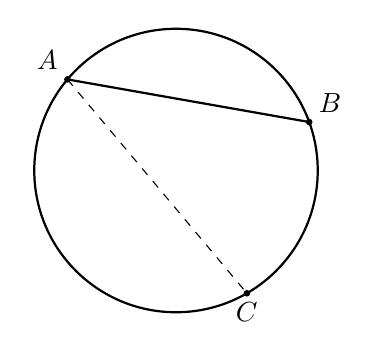
\begin{tikzpicture}
\draw[thick] (0,0) circle (1.80);
\coordinate (A) at (140:1.80);
\coordinate (B) at (20:1.80);
\coordinate (C) at (-60:1.80);
\draw[thick] (A)--(B);
\draw[dashed] (A)--(C);
\fill (A) circle(1.2pt) node[above left]{$A$};
\fill (B) circle(1.2pt) node[above right]{$B$};
\fill (C) circle(1.2pt) node[below]{$C$};
\end{tikzpicture}
    \CodeOutMid
    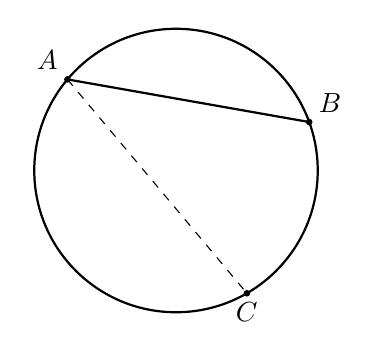
\begin{tikzpicture}
\draw[thick] (0,0) circle (1.80);
\coordinate (A) at (140:1.80);
\coordinate (B) at (20:1.80);
\coordinate (C) at (-60:1.80);
\draw[thick] (A)--(B);
\draw[dashed] (A)--(C);
\fill (A) circle(1.2pt) node[above left]{$A$};
\fill (B) circle(1.2pt) node[above right]{$B$};
\fill (C) circle(1.2pt) node[below]{$C$};
\end{tikzpicture}
    \CodeOutEnd
    \caption{G5) Konstruktsiya 5.}\label{fig:geo5}
    \CodeOutFigureEnd


    \subsection{G6) Konstruktsiya 6}
    \noindent\textbf{Maqsad.} Olimpiada chizmasida tez-tez uchraydigan skelet: kesishma/chord/tangent/ko‘pburchak yordamchi.

    \noindent\textbf{Konstruktsiya qadamlari.}
    \begin{enumerate}[leftmargin=*,itemsep=1pt]
\item Asosiy kontur (aylana yoki ko‘pburchak) ni chizing.
\item Yordamchi chiziq (diametr, chord, diagonal yoki tangent) ni qo‘shing.
\item Kerakli nuqtani kesishma/proyeksiya bilan oling.
\item Burchak/segment label va minimal belgilash qiling.
\end{enumerate}

    \CodeOutBegin
    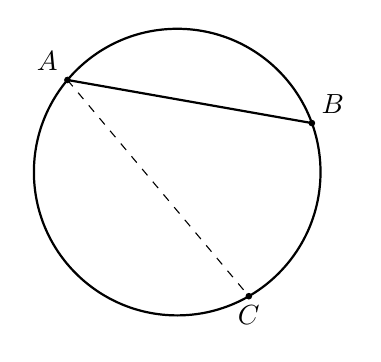
\begin{tikzpicture}
\draw[thick] (0,0) circle (1.82);
\coordinate (A) at (140:1.82);
\coordinate (B) at (20:1.82);
\coordinate (C) at (-60:1.82);
\draw[thick] (A)--(B);
\draw[dashed] (A)--(C);
\fill (A) circle(1.2pt) node[above left]{$A$};
\fill (B) circle(1.2pt) node[above right]{$B$};
\fill (C) circle(1.2pt) node[below]{$C$};
\end{tikzpicture}
    \CodeOutMid
    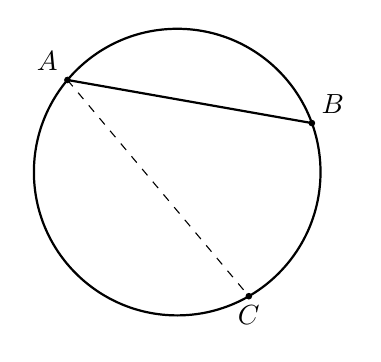
\begin{tikzpicture}
\draw[thick] (0,0) circle (1.82);
\coordinate (A) at (140:1.82);
\coordinate (B) at (20:1.82);
\coordinate (C) at (-60:1.82);
\draw[thick] (A)--(B);
\draw[dashed] (A)--(C);
\fill (A) circle(1.2pt) node[above left]{$A$};
\fill (B) circle(1.2pt) node[above right]{$B$};
\fill (C) circle(1.2pt) node[below]{$C$};
\end{tikzpicture}
    \CodeOutEnd
    \caption{G6) Konstruktsiya 6.}\label{fig:geo6}
    \CodeOutFigureEnd


    \subsection{G7) Konstruktsiya 7}
    \noindent\textbf{Maqsad.} Olimpiada chizmasida tez-tez uchraydigan skelet: kesishma/chord/tangent/ko‘pburchak yordamchi.

    \noindent\textbf{Konstruktsiya qadamlari.}
    \begin{enumerate}[leftmargin=*,itemsep=1pt]
\item Asosiy kontur (aylana yoki ko‘pburchak) ni chizing.
\item Yordamchi chiziq (diametr, chord, diagonal yoki tangent) ni qo‘shing.
\item Kerakli nuqtani kesishma/proyeksiya bilan oling.
\item Burchak/segment label va minimal belgilash qiling.
\end{enumerate}

    \CodeOutBegin
    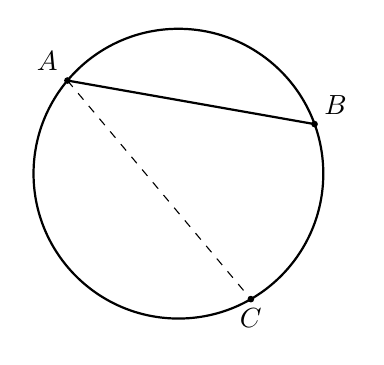
\begin{tikzpicture}
\draw[thick] (0,0) circle (1.84);
\coordinate (A) at (140:1.84);
\coordinate (B) at (20:1.84);
\coordinate (C) at (-60:1.84);
\draw[thick] (A)--(B);
\draw[dashed] (A)--(C);
\fill (A) circle(1.2pt) node[above left]{$A$};
\fill (B) circle(1.2pt) node[above right]{$B$};
\fill (C) circle(1.2pt) node[below]{$C$};
\end{tikzpicture}
    \CodeOutMid
    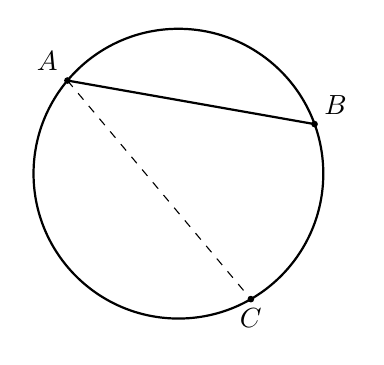
\begin{tikzpicture}
\draw[thick] (0,0) circle (1.84);
\coordinate (A) at (140:1.84);
\coordinate (B) at (20:1.84);
\coordinate (C) at (-60:1.84);
\draw[thick] (A)--(B);
\draw[dashed] (A)--(C);
\fill (A) circle(1.2pt) node[above left]{$A$};
\fill (B) circle(1.2pt) node[above right]{$B$};
\fill (C) circle(1.2pt) node[below]{$C$};
\end{tikzpicture}
    \CodeOutEnd
    \caption{G7) Konstruktsiya 7.}\label{fig:geo7}
    \CodeOutFigureEnd


    \subsection{G8) Konstruktsiya 8}
    \noindent\textbf{Maqsad.} Olimpiada chizmasida tez-tez uchraydigan skelet: kesishma/chord/tangent/ko‘pburchak yordamchi.

    \noindent\textbf{Konstruktsiya qadamlari.}
    \begin{enumerate}[leftmargin=*,itemsep=1pt]
\item Asosiy kontur (aylana yoki ko‘pburchak) ni chizing.
\item Yordamchi chiziq (diametr, chord, diagonal yoki tangent) ni qo‘shing.
\item Kerakli nuqtani kesishma/proyeksiya bilan oling.
\item Burchak/segment label va minimal belgilash qiling.
\end{enumerate}

    \CodeOutBegin
    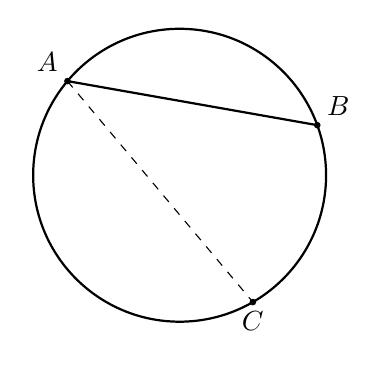
\begin{tikzpicture}
\draw[thick] (0,0) circle (1.86);
\coordinate (A) at (140:1.86);
\coordinate (B) at (20:1.86);
\coordinate (C) at (-60:1.86);
\draw[thick] (A)--(B);
\draw[dashed] (A)--(C);
\fill (A) circle(1.2pt) node[above left]{$A$};
\fill (B) circle(1.2pt) node[above right]{$B$};
\fill (C) circle(1.2pt) node[below]{$C$};
\end{tikzpicture}
    \CodeOutMid
    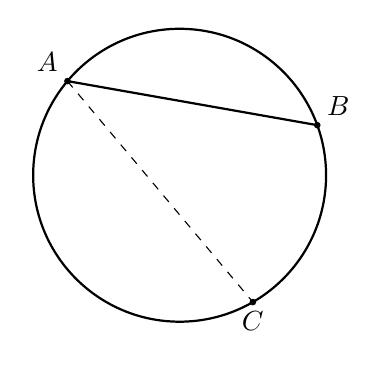
\begin{tikzpicture}
\draw[thick] (0,0) circle (1.86);
\coordinate (A) at (140:1.86);
\coordinate (B) at (20:1.86);
\coordinate (C) at (-60:1.86);
\draw[thick] (A)--(B);
\draw[dashed] (A)--(C);
\fill (A) circle(1.2pt) node[above left]{$A$};
\fill (B) circle(1.2pt) node[above right]{$B$};
\fill (C) circle(1.2pt) node[below]{$C$};
\end{tikzpicture}
    \CodeOutEnd
    \caption{G8) Konstruktsiya 8.}\label{fig:geo8}
    \CodeOutFigureEnd


    \subsection{G9) Konstruktsiya 9}
    \noindent\textbf{Maqsad.} Olimpiada chizmasida tez-tez uchraydigan skelet: kesishma/chord/tangent/ko‘pburchak yordamchi.

    \noindent\textbf{Konstruktsiya qadamlari.}
    \begin{enumerate}[leftmargin=*,itemsep=1pt]
\item Asosiy kontur (aylana yoki ko‘pburchak) ni chizing.
\item Yordamchi chiziq (diametr, chord, diagonal yoki tangent) ni qo‘shing.
\item Kerakli nuqtani kesishma/proyeksiya bilan oling.
\item Burchak/segment label va minimal belgilash qiling.
\end{enumerate}

    \CodeOutBegin
    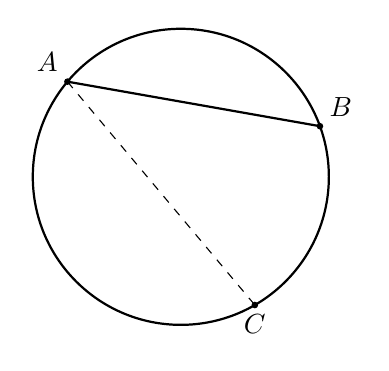
\begin{tikzpicture}
\draw[thick] (0,0) circle (1.88);
\coordinate (A) at (140:1.88);
\coordinate (B) at (20:1.88);
\coordinate (C) at (-60:1.88);
\draw[thick] (A)--(B);
\draw[dashed] (A)--(C);
\fill (A) circle(1.2pt) node[above left]{$A$};
\fill (B) circle(1.2pt) node[above right]{$B$};
\fill (C) circle(1.2pt) node[below]{$C$};
\end{tikzpicture}
    \CodeOutMid
    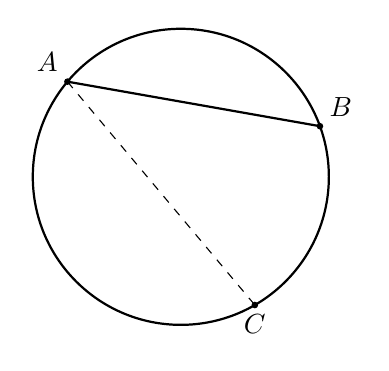
\begin{tikzpicture}
\draw[thick] (0,0) circle (1.88);
\coordinate (A) at (140:1.88);
\coordinate (B) at (20:1.88);
\coordinate (C) at (-60:1.88);
\draw[thick] (A)--(B);
\draw[dashed] (A)--(C);
\fill (A) circle(1.2pt) node[above left]{$A$};
\fill (B) circle(1.2pt) node[above right]{$B$};
\fill (C) circle(1.2pt) node[below]{$C$};
\end{tikzpicture}
    \CodeOutEnd
    \caption{G9) Konstruktsiya 9.}\label{fig:geo9}
    \CodeOutFigureEnd


    \subsection{G10) Konstruktsiya 10}
    \noindent\textbf{Maqsad.} Olimpiada chizmasida tez-tez uchraydigan skelet: kesishma/chord/tangent/ko‘pburchak yordamchi.

    \noindent\textbf{Konstruktsiya qadamlari.}
    \begin{enumerate}[leftmargin=*,itemsep=1pt]
\item Asosiy kontur (aylana yoki ko‘pburchak) ni chizing.
\item Yordamchi chiziq (diametr, chord, diagonal yoki tangent) ni qo‘shing.
\item Kerakli nuqtani kesishma/proyeksiya bilan oling.
\item Burchak/segment label va minimal belgilash qiling.
\end{enumerate}

    \CodeOutBegin
    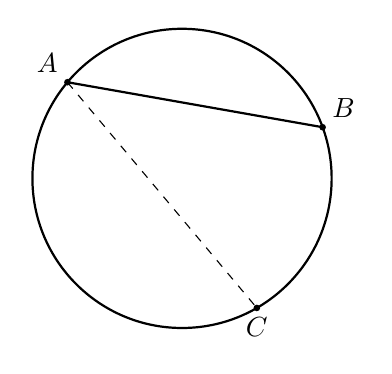
\begin{tikzpicture}
\draw[thick] (0,0) circle (1.90);
\coordinate (A) at (140:1.90);
\coordinate (B) at (20:1.90);
\coordinate (C) at (-60:1.90);
\draw[thick] (A)--(B);
\draw[dashed] (A)--(C);
\fill (A) circle(1.2pt) node[above left]{$A$};
\fill (B) circle(1.2pt) node[above right]{$B$};
\fill (C) circle(1.2pt) node[below]{$C$};
\end{tikzpicture}
    \CodeOutMid
    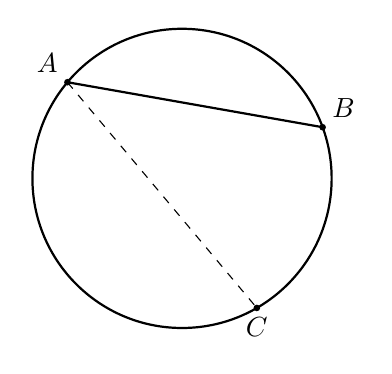
\begin{tikzpicture}
\draw[thick] (0,0) circle (1.90);
\coordinate (A) at (140:1.90);
\coordinate (B) at (20:1.90);
\coordinate (C) at (-60:1.90);
\draw[thick] (A)--(B);
\draw[dashed] (A)--(C);
\fill (A) circle(1.2pt) node[above left]{$A$};
\fill (B) circle(1.2pt) node[above right]{$B$};
\fill (C) circle(1.2pt) node[below]{$C$};
\end{tikzpicture}
    \CodeOutEnd
    \caption{G10) Konstruktsiya 10.}\label{fig:geo10}
    \CodeOutFigureEnd


    \subsection{G11) Konstruktsiya 11}
    \noindent\textbf{Maqsad.} Olimpiada chizmasida tez-tez uchraydigan skelet: kesishma/chord/tangent/ko‘pburchak yordamchi.

    \noindent\textbf{Konstruktsiya qadamlari.}
    \begin{enumerate}[leftmargin=*,itemsep=1pt]
\item Asosiy kontur (aylana yoki ko‘pburchak) ni chizing.
\item Yordamchi chiziq (diametr, chord, diagonal yoki tangent) ni qo‘shing.
\item Kerakli nuqtani kesishma/proyeksiya bilan oling.
\item Burchak/segment label va minimal belgilash qiling.
\end{enumerate}

    \CodeOutBegin
    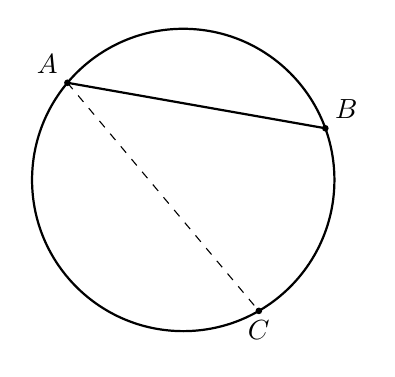
\begin{tikzpicture}
\draw[thick] (0,0) circle (1.92);
\coordinate (A) at (140:1.92);
\coordinate (B) at (20:1.92);
\coordinate (C) at (-60:1.92);
\draw[thick] (A)--(B);
\draw[dashed] (A)--(C);
\fill (A) circle(1.2pt) node[above left]{$A$};
\fill (B) circle(1.2pt) node[above right]{$B$};
\fill (C) circle(1.2pt) node[below]{$C$};
\end{tikzpicture}
    \CodeOutMid
    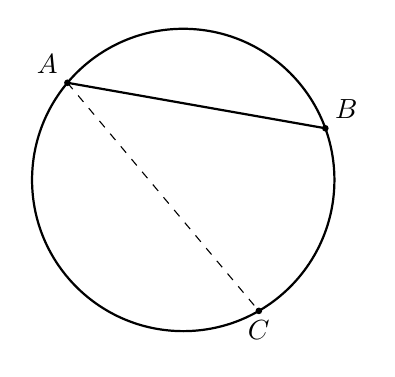
\begin{tikzpicture}
\draw[thick] (0,0) circle (1.92);
\coordinate (A) at (140:1.92);
\coordinate (B) at (20:1.92);
\coordinate (C) at (-60:1.92);
\draw[thick] (A)--(B);
\draw[dashed] (A)--(C);
\fill (A) circle(1.2pt) node[above left]{$A$};
\fill (B) circle(1.2pt) node[above right]{$B$};
\fill (C) circle(1.2pt) node[below]{$C$};
\end{tikzpicture}
    \CodeOutEnd
    \caption{G11) Konstruktsiya 11.}\label{fig:geo11}
    \CodeOutFigureEnd


    \subsection{G12) Konstruktsiya 12}
    \noindent\textbf{Maqsad.} Olimpiada chizmasida tez-tez uchraydigan skelet: kesishma/chord/tangent/ko‘pburchak yordamchi.

    \noindent\textbf{Konstruktsiya qadamlari.}
    \begin{enumerate}[leftmargin=*,itemsep=1pt]
\item Asosiy kontur (aylana yoki ko‘pburchak) ni chizing.
\item Yordamchi chiziq (diametr, chord, diagonal yoki tangent) ni qo‘shing.
\item Kerakli nuqtani kesishma/proyeksiya bilan oling.
\item Burchak/segment label va minimal belgilash qiling.
\end{enumerate}

    \CodeOutBegin
    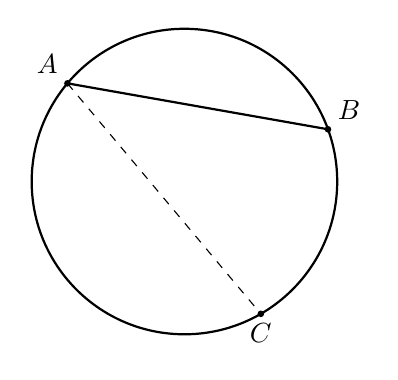
\begin{tikzpicture}
\draw[thick] (0,0) circle (1.94);
\coordinate (A) at (140:1.94);
\coordinate (B) at (20:1.94);
\coordinate (C) at (-60:1.94);
\draw[thick] (A)--(B);
\draw[dashed] (A)--(C);
\fill (A) circle(1.2pt) node[above left]{$A$};
\fill (B) circle(1.2pt) node[above right]{$B$};
\fill (C) circle(1.2pt) node[below]{$C$};
\end{tikzpicture}
    \CodeOutMid
    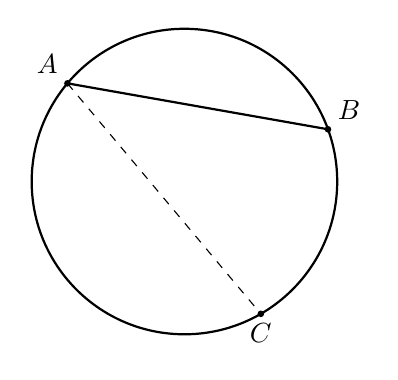
\begin{tikzpicture}
\draw[thick] (0,0) circle (1.94);
\coordinate (A) at (140:1.94);
\coordinate (B) at (20:1.94);
\coordinate (C) at (-60:1.94);
\draw[thick] (A)--(B);
\draw[dashed] (A)--(C);
\fill (A) circle(1.2pt) node[above left]{$A$};
\fill (B) circle(1.2pt) node[above right]{$B$};
\fill (C) circle(1.2pt) node[below]{$C$};
\end{tikzpicture}
    \CodeOutEnd
    \caption{G12) Konstruktsiya 12.}\label{fig:geo12}
    \CodeOutFigureEnd


    \subsection{G13) Konstruktsiya 13}
    \noindent\textbf{Maqsad.} Olimpiada chizmasida tez-tez uchraydigan skelet: kesishma/chord/tangent/ko‘pburchak yordamchi.

    \noindent\textbf{Konstruktsiya qadamlari.}
    \begin{enumerate}[leftmargin=*,itemsep=1pt]
\item Asosiy kontur (aylana yoki ko‘pburchak) ni chizing.
\item Yordamchi chiziq (diametr, chord, diagonal yoki tangent) ni qo‘shing.
\item Kerakli nuqtani kesishma/proyeksiya bilan oling.
\item Burchak/segment label va minimal belgilash qiling.
\end{enumerate}

    \CodeOutBegin
    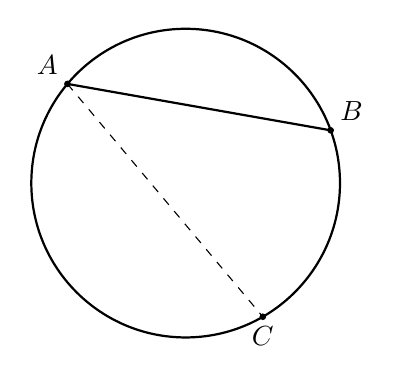
\begin{tikzpicture}
\draw[thick] (0,0) circle (1.96);
\coordinate (A) at (140:1.96);
\coordinate (B) at (20:1.96);
\coordinate (C) at (-60:1.96);
\draw[thick] (A)--(B);
\draw[dashed] (A)--(C);
\fill (A) circle(1.2pt) node[above left]{$A$};
\fill (B) circle(1.2pt) node[above right]{$B$};
\fill (C) circle(1.2pt) node[below]{$C$};
\end{tikzpicture}
    \CodeOutMid
    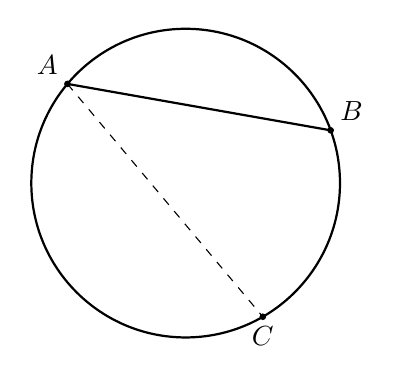
\begin{tikzpicture}
\draw[thick] (0,0) circle (1.96);
\coordinate (A) at (140:1.96);
\coordinate (B) at (20:1.96);
\coordinate (C) at (-60:1.96);
\draw[thick] (A)--(B);
\draw[dashed] (A)--(C);
\fill (A) circle(1.2pt) node[above left]{$A$};
\fill (B) circle(1.2pt) node[above right]{$B$};
\fill (C) circle(1.2pt) node[below]{$C$};
\end{tikzpicture}
    \CodeOutEnd
    \caption{G13) Konstruktsiya 13.}\label{fig:geo13}
    \CodeOutFigureEnd


    \subsection{G14) Konstruktsiya 14}
    \noindent\textbf{Maqsad.} Olimpiada chizmasida tez-tez uchraydigan skelet: kesishma/chord/tangent/ko‘pburchak yordamchi.

    \noindent\textbf{Konstruktsiya qadamlari.}
    \begin{enumerate}[leftmargin=*,itemsep=1pt]
\item Asosiy kontur (aylana yoki ko‘pburchak) ni chizing.
\item Yordamchi chiziq (diametr, chord, diagonal yoki tangent) ni qo‘shing.
\item Kerakli nuqtani kesishma/proyeksiya bilan oling.
\item Burchak/segment label va minimal belgilash qiling.
\end{enumerate}

    \CodeOutBegin
    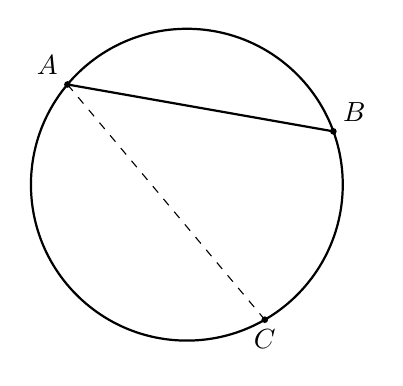
\begin{tikzpicture}
\draw[thick] (0,0) circle (1.98);
\coordinate (A) at (140:1.98);
\coordinate (B) at (20:1.98);
\coordinate (C) at (-60:1.98);
\draw[thick] (A)--(B);
\draw[dashed] (A)--(C);
\fill (A) circle(1.2pt) node[above left]{$A$};
\fill (B) circle(1.2pt) node[above right]{$B$};
\fill (C) circle(1.2pt) node[below]{$C$};
\end{tikzpicture}
    \CodeOutMid
    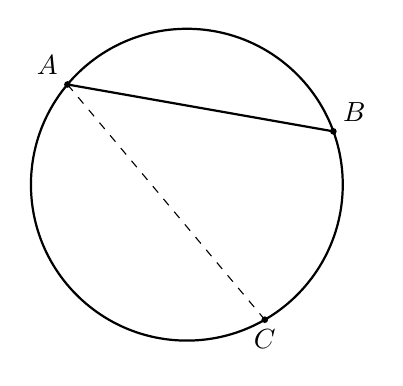
\begin{tikzpicture}
\draw[thick] (0,0) circle (1.98);
\coordinate (A) at (140:1.98);
\coordinate (B) at (20:1.98);
\coordinate (C) at (-60:1.98);
\draw[thick] (A)--(B);
\draw[dashed] (A)--(C);
\fill (A) circle(1.2pt) node[above left]{$A$};
\fill (B) circle(1.2pt) node[above right]{$B$};
\fill (C) circle(1.2pt) node[below]{$C$};
\end{tikzpicture}
    \CodeOutEnd
    \caption{G14) Konstruktsiya 14.}\label{fig:geo14}
    \CodeOutFigureEnd


    \subsection{G15) Konstruktsiya 15}
    \noindent\textbf{Maqsad.} Olimpiada chizmasida tez-tez uchraydigan skelet: kesishma/chord/tangent/ko‘pburchak yordamchi.

    \noindent\textbf{Konstruktsiya qadamlari.}
    \begin{enumerate}[leftmargin=*,itemsep=1pt]
\item Asosiy kontur (aylana yoki ko‘pburchak) ni chizing.
\item Yordamchi chiziq (diametr, chord, diagonal yoki tangent) ni qo‘shing.
\item Kerakli nuqtani kesishma/proyeksiya bilan oling.
\item Burchak/segment label va minimal belgilash qiling.
\end{enumerate}

    \CodeOutBegin
    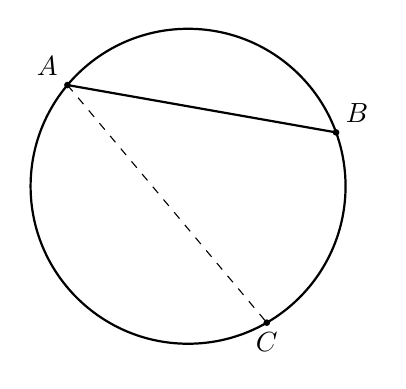
\begin{tikzpicture}
\draw[thick] (0,0) circle (2.00);
\coordinate (A) at (140:2.00);
\coordinate (B) at (20:2.00);
\coordinate (C) at (-60:2.00);
\draw[thick] (A)--(B);
\draw[dashed] (A)--(C);
\fill (A) circle(1.2pt) node[above left]{$A$};
\fill (B) circle(1.2pt) node[above right]{$B$};
\fill (C) circle(1.2pt) node[below]{$C$};
\end{tikzpicture}
    \CodeOutMid
    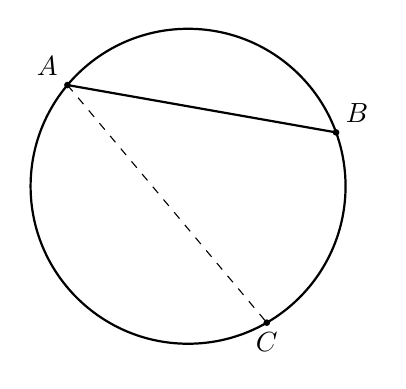
\begin{tikzpicture}
\draw[thick] (0,0) circle (2.00);
\coordinate (A) at (140:2.00);
\coordinate (B) at (20:2.00);
\coordinate (C) at (-60:2.00);
\draw[thick] (A)--(B);
\draw[dashed] (A)--(C);
\fill (A) circle(1.2pt) node[above left]{$A$};
\fill (B) circle(1.2pt) node[above right]{$B$};
\fill (C) circle(1.2pt) node[below]{$C$};
\end{tikzpicture}
    \CodeOutEnd
    \caption{G15) Konstruktsiya 15.}\label{fig:geo15}
    \CodeOutFigureEnd


    \subsection{G16) Konstruktsiya 16}
    \noindent\textbf{Maqsad.} Olimpiada chizmasida tez-tez uchraydigan skelet: kesishma/chord/tangent/ko‘pburchak yordamchi.

    \noindent\textbf{Konstruktsiya qadamlari.}
    \begin{enumerate}[leftmargin=*,itemsep=1pt]
\item Asosiy kontur (aylana yoki ko‘pburchak) ni chizing.
\item Yordamchi chiziq (diametr, chord, diagonal yoki tangent) ni qo‘shing.
\item Kerakli nuqtani kesishma/proyeksiya bilan oling.
\item Burchak/segment label va minimal belgilash qiling.
\end{enumerate}

    \CodeOutBegin
    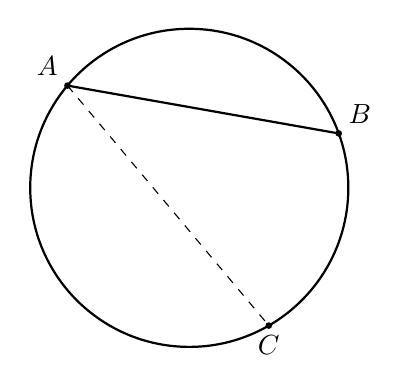
\begin{tikzpicture}
\draw[thick] (0,0) circle (2.02);
\coordinate (A) at (140:2.02);
\coordinate (B) at (20:2.02);
\coordinate (C) at (-60:2.02);
\draw[thick] (A)--(B);
\draw[dashed] (A)--(C);
\fill (A) circle(1.2pt) node[above left]{$A$};
\fill (B) circle(1.2pt) node[above right]{$B$};
\fill (C) circle(1.2pt) node[below]{$C$};
\end{tikzpicture}
    \CodeOutMid
    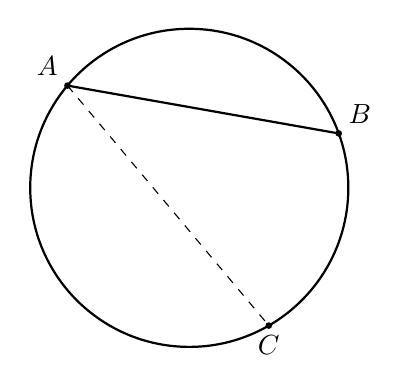
\begin{tikzpicture}
\draw[thick] (0,0) circle (2.02);
\coordinate (A) at (140:2.02);
\coordinate (B) at (20:2.02);
\coordinate (C) at (-60:2.02);
\draw[thick] (A)--(B);
\draw[dashed] (A)--(C);
\fill (A) circle(1.2pt) node[above left]{$A$};
\fill (B) circle(1.2pt) node[above right]{$B$};
\fill (C) circle(1.2pt) node[below]{$C$};
\end{tikzpicture}
    \CodeOutEnd
    \caption{G16) Konstruktsiya 16.}\label{fig:geo16}
    \CodeOutFigureEnd


    \subsection{G17) Konstruktsiya 17}
    \noindent\textbf{Maqsad.} Olimpiada chizmasida tez-tez uchraydigan skelet: kesishma/chord/tangent/ko‘pburchak yordamchi.

    \noindent\textbf{Konstruktsiya qadamlari.}
    \begin{enumerate}[leftmargin=*,itemsep=1pt]
\item Asosiy kontur (aylana yoki ko‘pburchak) ni chizing.
\item Yordamchi chiziq (diametr, chord, diagonal yoki tangent) ni qo‘shing.
\item Kerakli nuqtani kesishma/proyeksiya bilan oling.
\item Burchak/segment label va minimal belgilash qiling.
\end{enumerate}

    \CodeOutBegin
    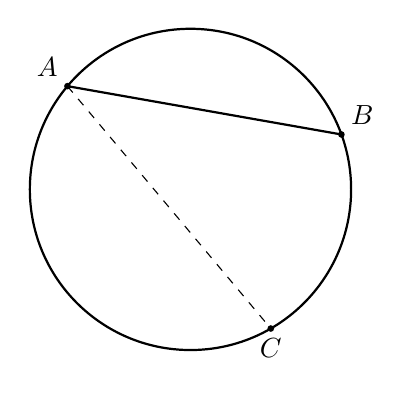
\begin{tikzpicture}
\draw[thick] (0,0) circle (2.04);
\coordinate (A) at (140:2.04);
\coordinate (B) at (20:2.04);
\coordinate (C) at (-60:2.04);
\draw[thick] (A)--(B);
\draw[dashed] (A)--(C);
\fill (A) circle(1.2pt) node[above left]{$A$};
\fill (B) circle(1.2pt) node[above right]{$B$};
\fill (C) circle(1.2pt) node[below]{$C$};
\end{tikzpicture}
    \CodeOutMid
    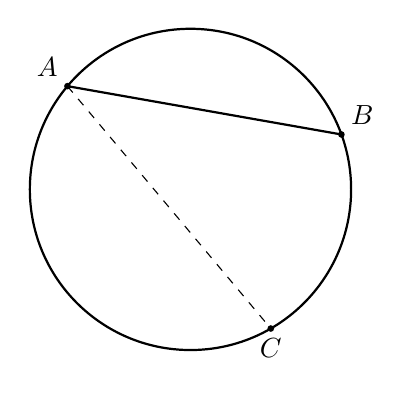
\begin{tikzpicture}
\draw[thick] (0,0) circle (2.04);
\coordinate (A) at (140:2.04);
\coordinate (B) at (20:2.04);
\coordinate (C) at (-60:2.04);
\draw[thick] (A)--(B);
\draw[dashed] (A)--(C);
\fill (A) circle(1.2pt) node[above left]{$A$};
\fill (B) circle(1.2pt) node[above right]{$B$};
\fill (C) circle(1.2pt) node[below]{$C$};
\end{tikzpicture}
    \CodeOutEnd
    \caption{G17) Konstruktsiya 17.}\label{fig:geo17}
    \CodeOutFigureEnd


    \subsection{G18) Konstruktsiya 18}
    \noindent\textbf{Maqsad.} Olimpiada chizmasida tez-tez uchraydigan skelet: kesishma/chord/tangent/ko‘pburchak yordamchi.

    \noindent\textbf{Konstruktsiya qadamlari.}
    \begin{enumerate}[leftmargin=*,itemsep=1pt]
\item Asosiy kontur (aylana yoki ko‘pburchak) ni chizing.
\item Yordamchi chiziq (diametr, chord, diagonal yoki tangent) ni qo‘shing.
\item Kerakli nuqtani kesishma/proyeksiya bilan oling.
\item Burchak/segment label va minimal belgilash qiling.
\end{enumerate}

    \CodeOutBegin
    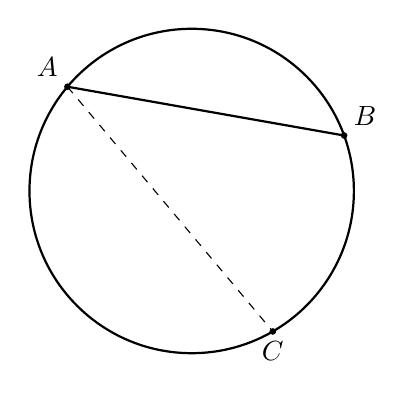
\begin{tikzpicture}
\draw[thick] (0,0) circle (2.06);
\coordinate (A) at (140:2.06);
\coordinate (B) at (20:2.06);
\coordinate (C) at (-60:2.06);
\draw[thick] (A)--(B);
\draw[dashed] (A)--(C);
\fill (A) circle(1.2pt) node[above left]{$A$};
\fill (B) circle(1.2pt) node[above right]{$B$};
\fill (C) circle(1.2pt) node[below]{$C$};
\end{tikzpicture}
    \CodeOutMid
    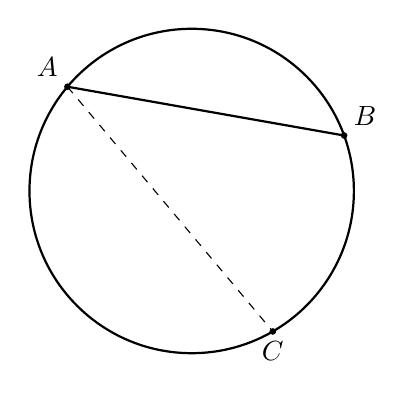
\begin{tikzpicture}
\draw[thick] (0,0) circle (2.06);
\coordinate (A) at (140:2.06);
\coordinate (B) at (20:2.06);
\coordinate (C) at (-60:2.06);
\draw[thick] (A)--(B);
\draw[dashed] (A)--(C);
\fill (A) circle(1.2pt) node[above left]{$A$};
\fill (B) circle(1.2pt) node[above right]{$B$};
\fill (C) circle(1.2pt) node[below]{$C$};
\end{tikzpicture}
    \CodeOutEnd
    \caption{G18) Konstruktsiya 18.}\label{fig:geo18}
    \CodeOutFigureEnd


    \subsection{G19) Konstruktsiya 19}
    \noindent\textbf{Maqsad.} Olimpiada chizmasida tez-tez uchraydigan skelet: kesishma/chord/tangent/ko‘pburchak yordamchi.

    \noindent\textbf{Konstruktsiya qadamlari.}
    \begin{enumerate}[leftmargin=*,itemsep=1pt]
\item Asosiy kontur (aylana yoki ko‘pburchak) ni chizing.
\item Yordamchi chiziq (diametr, chord, diagonal yoki tangent) ni qo‘shing.
\item Kerakli nuqtani kesishma/proyeksiya bilan oling.
\item Burchak/segment label va minimal belgilash qiling.
\end{enumerate}

    \CodeOutBegin
    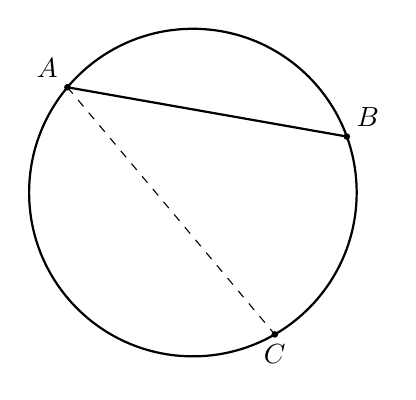
\begin{tikzpicture}
\draw[thick] (0,0) circle (2.08);
\coordinate (A) at (140:2.08);
\coordinate (B) at (20:2.08);
\coordinate (C) at (-60:2.08);
\draw[thick] (A)--(B);
\draw[dashed] (A)--(C);
\fill (A) circle(1.2pt) node[above left]{$A$};
\fill (B) circle(1.2pt) node[above right]{$B$};
\fill (C) circle(1.2pt) node[below]{$C$};
\end{tikzpicture}
    \CodeOutMid
    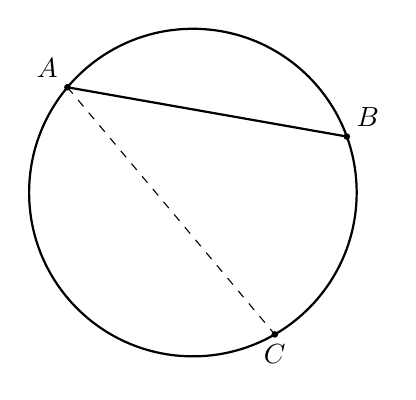
\begin{tikzpicture}
\draw[thick] (0,0) circle (2.08);
\coordinate (A) at (140:2.08);
\coordinate (B) at (20:2.08);
\coordinate (C) at (-60:2.08);
\draw[thick] (A)--(B);
\draw[dashed] (A)--(C);
\fill (A) circle(1.2pt) node[above left]{$A$};
\fill (B) circle(1.2pt) node[above right]{$B$};
\fill (C) circle(1.2pt) node[below]{$C$};
\end{tikzpicture}
    \CodeOutEnd
    \caption{G19) Konstruktsiya 19.}\label{fig:geo19}
    \CodeOutFigureEnd


    \subsection{G20) Konstruktsiya 20}
    \noindent\textbf{Maqsad.} Olimpiada chizmasida tez-tez uchraydigan skelet: kesishma/chord/tangent/ko‘pburchak yordamchi.

    \noindent\textbf{Konstruktsiya qadamlari.}
    \begin{enumerate}[leftmargin=*,itemsep=1pt]
\item Asosiy kontur (aylana yoki ko‘pburchak) ni chizing.
\item Yordamchi chiziq (diametr, chord, diagonal yoki tangent) ni qo‘shing.
\item Kerakli nuqtani kesishma/proyeksiya bilan oling.
\item Burchak/segment label va minimal belgilash qiling.
\end{enumerate}

    \CodeOutBegin
    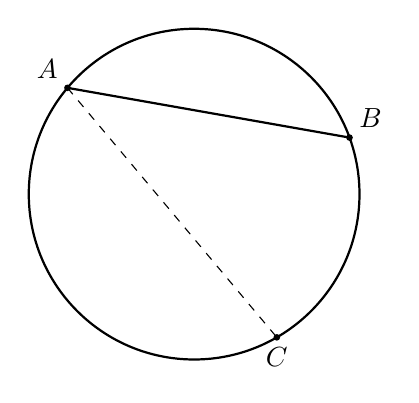
\begin{tikzpicture}
\draw[thick] (0,0) circle (2.10);
\coordinate (A) at (140:2.10);
\coordinate (B) at (20:2.10);
\coordinate (C) at (-60:2.10);
\draw[thick] (A)--(B);
\draw[dashed] (A)--(C);
\fill (A) circle(1.2pt) node[above left]{$A$};
\fill (B) circle(1.2pt) node[above right]{$B$};
\fill (C) circle(1.2pt) node[below]{$C$};
\end{tikzpicture}
    \CodeOutMid
    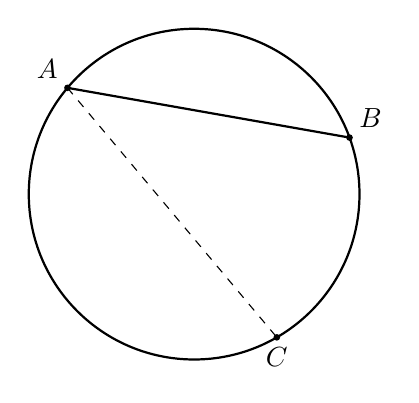
\begin{tikzpicture}
\draw[thick] (0,0) circle (2.10);
\coordinate (A) at (140:2.10);
\coordinate (B) at (20:2.10);
\coordinate (C) at (-60:2.10);
\draw[thick] (A)--(B);
\draw[dashed] (A)--(C);
\fill (A) circle(1.2pt) node[above left]{$A$};
\fill (B) circle(1.2pt) node[above right]{$B$};
\fill (C) circle(1.2pt) node[below]{$C$};
\end{tikzpicture}
    \CodeOutEnd
    \caption{G20) Konstruktsiya 20.}\label{fig:geo20}
    \CodeOutFigureEnd

\section{Olimpiada 2D chizmalari (40 ta) — kategoriyalar bo‘yicha}

    \subsection{O1) Olimpiada 2D — konfiguratsiya 1}
    \noindent\textbf{Maqsad.} Yordamchi chiziq tanlash: chord/tangent/diagonal/parallel/sikliklikni ko‘rsatish.

    \noindent\textbf{Konstruktsiya qadamlari.}
    \begin{enumerate}[leftmargin=*,itemsep=1pt]
\item Skeletni chizing (aylana yoki to‘rtburchak/ko‘pburchak).
\item Shartdagi elementni qo‘shing (tangent yoki diagonal yoki parallel).
\item Kesishmani aniq belgilang (name intersections yoki proyeksiya).
\item Isbotda ishlatiladigan burchak/segmentlarni label qiling.
\end{enumerate}

    \CodeOutBegin
    \begin{tikzpicture}
\coordinate (O) at (0,0);
\draw[thick] (O) circle (2.1);
\coordinate (T) at (250:2.1);
\coordinate (A) at (140:2.1);
\coordinate (B) at (20:2.1);
\draw[thick] (A)--(B);
\draw[thick] (T) -- ($(T)!1!90:(O)$);
\draw[dashed] (O)--(T);
\fill (T) circle(1.2pt) node[below]{$T$};
\end{tikzpicture}
    \CodeOutMid
    \begin{tikzpicture}
\coordinate (O) at (0,0);
\draw[thick] (O) circle (2.1);
\coordinate (T) at (250:2.1);
\coordinate (A) at (140:2.1);
\coordinate (B) at (20:2.1);
\draw[thick] (A)--(B);
\draw[thick] (T) -- ($(T)!1!90:(O)$);
\draw[dashed] (O)--(T);
\fill (T) circle(1.2pt) node[below]{$T$};
\end{tikzpicture}
    \CodeOutEnd
    \caption{O1) Olimpiada 2D — konfiguratsiya 1.}\label{fig:ol2d1}
    \CodeOutFigureEnd


    \subsection{O2) Olimpiada 2D — konfiguratsiya 2}
    \noindent\textbf{Maqsad.} Yordamchi chiziq tanlash: chord/tangent/diagonal/parallel/sikliklikni ko‘rsatish.

    \noindent\textbf{Konstruktsiya qadamlari.}
    \begin{enumerate}[leftmargin=*,itemsep=1pt]
\item Skeletni chizing (aylana yoki to‘rtburchak/ko‘pburchak).
\item Shartdagi elementni qo‘shing (tangent yoki diagonal yoki parallel).
\item Kesishmani aniq belgilang (name intersections yoki proyeksiya).
\item Isbotda ishlatiladigan burchak/segmentlarni label qiling.
\end{enumerate}

    \CodeOutBegin
    \begin{tikzpicture}
\draw[thick] (0,0) circle (2.02);
\coordinate (A) at (130:2.02);
\coordinate (B) at (40:2.02);
\coordinate (C) at (-20:2.02);
\coordinate (D) at (-120:2.02);
\draw[thick] (A)--(B)--(C)--(D)--cycle;
\draw[dashed] (A)--(C);
\end{tikzpicture}
    \CodeOutMid
    \begin{tikzpicture}
\draw[thick] (0,0) circle (2.02);
\coordinate (A) at (130:2.02);
\coordinate (B) at (40:2.02);
\coordinate (C) at (-20:2.02);
\coordinate (D) at (-120:2.02);
\draw[thick] (A)--(B)--(C)--(D)--cycle;
\draw[dashed] (A)--(C);
\end{tikzpicture}
    \CodeOutEnd
    \caption{O2) Olimpiada 2D — konfiguratsiya 2.}\label{fig:ol2d2}
    \CodeOutFigureEnd


    \subsection{O3) Olimpiada 2D — konfiguratsiya 3}
    \noindent\textbf{Maqsad.} Yordamchi chiziq tanlash: chord/tangent/diagonal/parallel/sikliklikni ko‘rsatish.

    \noindent\textbf{Konstruktsiya qadamlari.}
    \begin{enumerate}[leftmargin=*,itemsep=1pt]
\item Skeletni chizing (aylana yoki to‘rtburchak/ko‘pburchak).
\item Shartdagi elementni qo‘shing (tangent yoki diagonal yoki parallel).
\item Kesishmani aniq belgilang (name intersections yoki proyeksiya).
\item Isbotda ishlatiladigan burchak/segmentlarni label qiling.
\end{enumerate}

    \CodeOutBegin
    \begin{tikzpicture}
\coordinate (A) at (0,0);
\coordinate (B) at (5,0);
\coordinate (D) at (1.2,2.4);
\coordinate (C) at (4.0,2.4);
\draw[thick] (A)--(B)--(C)--(D)--cycle;
\draw[dashed] (A)--(C);
\draw[dashed] (B)--(D);
\end{tikzpicture}
    \CodeOutMid
    \begin{tikzpicture}
\coordinate (A) at (0,0);
\coordinate (B) at (5,0);
\coordinate (D) at (1.2,2.4);
\coordinate (C) at (4.0,2.4);
\draw[thick] (A)--(B)--(C)--(D)--cycle;
\draw[dashed] (A)--(C);
\draw[dashed] (B)--(D);
\end{tikzpicture}
    \CodeOutEnd
    \caption{O3) Olimpiada 2D — konfiguratsiya 3.}\label{fig:ol2d3}
    \CodeOutFigureEnd


    \subsection{O4) Olimpiada 2D — konfiguratsiya 4}
    \noindent\textbf{Maqsad.} Yordamchi chiziq tanlash: chord/tangent/diagonal/parallel/sikliklikni ko‘rsatish.

    \noindent\textbf{Konstruktsiya qadamlari.}
    \begin{enumerate}[leftmargin=*,itemsep=1pt]
\item Skeletni chizing (aylana yoki to‘rtburchak/ko‘pburchak).
\item Shartdagi elementni qo‘shing (tangent yoki diagonal yoki parallel).
\item Kesishmani aniq belgilang (name intersections yoki proyeksiya).
\item Isbotda ishlatiladigan burchak/segmentlarni label qiling.
\end{enumerate}

    \CodeOutBegin
    \begin{tikzpicture}
\coordinate (A) at (0,0);
\coordinate (B) at (4.5,0);
\coordinate (D) at (1.2,2.2);
\coordinate (C) at ($(B)+(D)-(A)$);
\draw[thick] (A)--(B)--(C)--(D)--cycle;
\draw[dashed] (A)--(C);
\draw[dashed] (B)--(D);
\end{tikzpicture}
    \CodeOutMid
    \begin{tikzpicture}
\coordinate (A) at (0,0);
\coordinate (B) at (4.5,0);
\coordinate (D) at (1.2,2.2);
\coordinate (C) at ($(B)+(D)-(A)$);
\draw[thick] (A)--(B)--(C)--(D)--cycle;
\draw[dashed] (A)--(C);
\draw[dashed] (B)--(D);
\end{tikzpicture}
    \CodeOutEnd
    \caption{O4) Olimpiada 2D — konfiguratsiya 4.}\label{fig:ol2d4}
    \CodeOutFigureEnd


    \subsection{O5) Olimpiada 2D — konfiguratsiya 5}
    \noindent\textbf{Maqsad.} Yordamchi chiziq tanlash: chord/tangent/diagonal/parallel/sikliklikni ko‘rsatish.

    \noindent\textbf{Konstruktsiya qadamlari.}
    \begin{enumerate}[leftmargin=*,itemsep=1pt]
\item Skeletni chizing (aylana yoki to‘rtburchak/ko‘pburchak).
\item Shartdagi elementni qo‘shing (tangent yoki diagonal yoki parallel).
\item Kesishmani aniq belgilang (name intersections yoki proyeksiya).
\item Isbotda ishlatiladigan burchak/segmentlarni label qiling.
\end{enumerate}

    \CodeOutBegin
    \begin{tikzpicture}
\coordinate (P1) at (0,0);
\coordinate (P2) at (3.2,-0.2);
\coordinate (P3) at (5.0,1.8);
\coordinate (P4) at (3.8,4.0);
\coordinate (P5) at (1.4,4.2);
\draw[thick] (P1)--(P2)--(P3)--(P4)--(P5)--cycle;
\draw[dashed] (P1)--(P3);
\draw[dashed] (P1)--(P4);
\end{tikzpicture}
    \CodeOutMid
    \begin{tikzpicture}
\coordinate (P1) at (0,0);
\coordinate (P2) at (3.2,-0.2);
\coordinate (P3) at (5.0,1.8);
\coordinate (P4) at (3.8,4.0);
\coordinate (P5) at (1.4,4.2);
\draw[thick] (P1)--(P2)--(P3)--(P4)--(P5)--cycle;
\draw[dashed] (P1)--(P3);
\draw[dashed] (P1)--(P4);
\end{tikzpicture}
    \CodeOutEnd
    \caption{O5) Olimpiada 2D — konfiguratsiya 5.}\label{fig:ol2d5}
    \CodeOutFigureEnd


    \subsection{O6) Olimpiada 2D — konfiguratsiya 6}
    \noindent\textbf{Maqsad.} Yordamchi chiziq tanlash: chord/tangent/diagonal/parallel/sikliklikni ko‘rsatish.

    \noindent\textbf{Konstruktsiya qadamlari.}
    \begin{enumerate}[leftmargin=*,itemsep=1pt]
\item Skeletni chizing (aylana yoki to‘rtburchak/ko‘pburchak).
\item Shartdagi elementni qo‘shing (tangent yoki diagonal yoki parallel).
\item Kesishmani aniq belgilang (name intersections yoki proyeksiya).
\item Isbotda ishlatiladigan burchak/segmentlarni label qiling.
\end{enumerate}

    \CodeOutBegin
    \begin{tikzpicture}
\coordinate (O) at (0,0);
\draw[thick] (O) circle (2.1);
\coordinate (T) at (250:2.1);
\coordinate (A) at (140:2.1);
\coordinate (B) at (20:2.1);
\draw[thick] (A)--(B);
\draw[thick] (T) -- ($(T)!1!90:(O)$);
\draw[dashed] (O)--(T);
\fill (T) circle(1.2pt) node[below]{$T$};
\end{tikzpicture}
    \CodeOutMid
    \begin{tikzpicture}
\coordinate (O) at (0,0);
\draw[thick] (O) circle (2.1);
\coordinate (T) at (250:2.1);
\coordinate (A) at (140:2.1);
\coordinate (B) at (20:2.1);
\draw[thick] (A)--(B);
\draw[thick] (T) -- ($(T)!1!90:(O)$);
\draw[dashed] (O)--(T);
\fill (T) circle(1.2pt) node[below]{$T$};
\end{tikzpicture}
    \CodeOutEnd
    \caption{O6) Olimpiada 2D — konfiguratsiya 6.}\label{fig:ol2d6}
    \CodeOutFigureEnd


    \subsection{O7) Olimpiada 2D — konfiguratsiya 7}
    \noindent\textbf{Maqsad.} Yordamchi chiziq tanlash: chord/tangent/diagonal/parallel/sikliklikni ko‘rsatish.

    \noindent\textbf{Konstruktsiya qadamlari.}
    \begin{enumerate}[leftmargin=*,itemsep=1pt]
\item Skeletni chizing (aylana yoki to‘rtburchak/ko‘pburchak).
\item Shartdagi elementni qo‘shing (tangent yoki diagonal yoki parallel).
\item Kesishmani aniq belgilang (name intersections yoki proyeksiya).
\item Isbotda ishlatiladigan burchak/segmentlarni label qiling.
\end{enumerate}

    \CodeOutBegin
    \begin{tikzpicture}
\draw[thick] (0,0) circle (2.07);
\coordinate (A) at (130:2.07);
\coordinate (B) at (40:2.07);
\coordinate (C) at (-20:2.07);
\coordinate (D) at (-120:2.07);
\draw[thick] (A)--(B)--(C)--(D)--cycle;
\draw[dashed] (A)--(C);
\end{tikzpicture}
    \CodeOutMid
    \begin{tikzpicture}
\draw[thick] (0,0) circle (2.07);
\coordinate (A) at (130:2.07);
\coordinate (B) at (40:2.07);
\coordinate (C) at (-20:2.07);
\coordinate (D) at (-120:2.07);
\draw[thick] (A)--(B)--(C)--(D)--cycle;
\draw[dashed] (A)--(C);
\end{tikzpicture}
    \CodeOutEnd
    \caption{O7) Olimpiada 2D — konfiguratsiya 7.}\label{fig:ol2d7}
    \CodeOutFigureEnd


    \subsection{O8) Olimpiada 2D — konfiguratsiya 8}
    \noindent\textbf{Maqsad.} Yordamchi chiziq tanlash: chord/tangent/diagonal/parallel/sikliklikni ko‘rsatish.

    \noindent\textbf{Konstruktsiya qadamlari.}
    \begin{enumerate}[leftmargin=*,itemsep=1pt]
\item Skeletni chizing (aylana yoki to‘rtburchak/ko‘pburchak).
\item Shartdagi elementni qo‘shing (tangent yoki diagonal yoki parallel).
\item Kesishmani aniq belgilang (name intersections yoki proyeksiya).
\item Isbotda ishlatiladigan burchak/segmentlarni label qiling.
\end{enumerate}

    \CodeOutBegin
    \begin{tikzpicture}
\coordinate (A) at (0,0);
\coordinate (B) at (5,0);
\coordinate (D) at (1.2,2.4);
\coordinate (C) at (4.0,2.4);
\draw[thick] (A)--(B)--(C)--(D)--cycle;
\draw[dashed] (A)--(C);
\draw[dashed] (B)--(D);
\end{tikzpicture}
    \CodeOutMid
    \begin{tikzpicture}
\coordinate (A) at (0,0);
\coordinate (B) at (5,0);
\coordinate (D) at (1.2,2.4);
\coordinate (C) at (4.0,2.4);
\draw[thick] (A)--(B)--(C)--(D)--cycle;
\draw[dashed] (A)--(C);
\draw[dashed] (B)--(D);
\end{tikzpicture}
    \CodeOutEnd
    \caption{O8) Olimpiada 2D — konfiguratsiya 8.}\label{fig:ol2d8}
    \CodeOutFigureEnd


    \subsection{O9) Olimpiada 2D — konfiguratsiya 9}
    \noindent\textbf{Maqsad.} Yordamchi chiziq tanlash: chord/tangent/diagonal/parallel/sikliklikni ko‘rsatish.

    \noindent\textbf{Konstruktsiya qadamlari.}
    \begin{enumerate}[leftmargin=*,itemsep=1pt]
\item Skeletni chizing (aylana yoki to‘rtburchak/ko‘pburchak).
\item Shartdagi elementni qo‘shing (tangent yoki diagonal yoki parallel).
\item Kesishmani aniq belgilang (name intersections yoki proyeksiya).
\item Isbotda ishlatiladigan burchak/segmentlarni label qiling.
\end{enumerate}

    \CodeOutBegin
    \begin{tikzpicture}
\coordinate (A) at (0,0);
\coordinate (B) at (4.5,0);
\coordinate (D) at (1.2,2.2);
\coordinate (C) at ($(B)+(D)-(A)$);
\draw[thick] (A)--(B)--(C)--(D)--cycle;
\draw[dashed] (A)--(C);
\draw[dashed] (B)--(D);
\end{tikzpicture}
    \CodeOutMid
    \begin{tikzpicture}
\coordinate (A) at (0,0);
\coordinate (B) at (4.5,0);
\coordinate (D) at (1.2,2.2);
\coordinate (C) at ($(B)+(D)-(A)$);
\draw[thick] (A)--(B)--(C)--(D)--cycle;
\draw[dashed] (A)--(C);
\draw[dashed] (B)--(D);
\end{tikzpicture}
    \CodeOutEnd
    \caption{O9) Olimpiada 2D — konfiguratsiya 9.}\label{fig:ol2d9}
    \CodeOutFigureEnd


    \subsection{O10) Olimpiada 2D — konfiguratsiya 10}
    \noindent\textbf{Maqsad.} Yordamchi chiziq tanlash: chord/tangent/diagonal/parallel/sikliklikni ko‘rsatish.

    \noindent\textbf{Konstruktsiya qadamlari.}
    \begin{enumerate}[leftmargin=*,itemsep=1pt]
\item Skeletni chizing (aylana yoki to‘rtburchak/ko‘pburchak).
\item Shartdagi elementni qo‘shing (tangent yoki diagonal yoki parallel).
\item Kesishmani aniq belgilang (name intersections yoki proyeksiya).
\item Isbotda ishlatiladigan burchak/segmentlarni label qiling.
\end{enumerate}

    \CodeOutBegin
    \begin{tikzpicture}
\coordinate (P1) at (0,0);
\coordinate (P2) at (3.2,-0.2);
\coordinate (P3) at (5.0,1.8);
\coordinate (P4) at (3.8,4.0);
\coordinate (P5) at (1.4,4.2);
\draw[thick] (P1)--(P2)--(P3)--(P4)--(P5)--cycle;
\draw[dashed] (P1)--(P3);
\draw[dashed] (P1)--(P4);
\end{tikzpicture}
    \CodeOutMid
    \begin{tikzpicture}
\coordinate (P1) at (0,0);
\coordinate (P2) at (3.2,-0.2);
\coordinate (P3) at (5.0,1.8);
\coordinate (P4) at (3.8,4.0);
\coordinate (P5) at (1.4,4.2);
\draw[thick] (P1)--(P2)--(P3)--(P4)--(P5)--cycle;
\draw[dashed] (P1)--(P3);
\draw[dashed] (P1)--(P4);
\end{tikzpicture}
    \CodeOutEnd
    \caption{O10) Olimpiada 2D — konfiguratsiya 10.}\label{fig:ol2d10}
    \CodeOutFigureEnd


    \subsection{O11) Olimpiada 2D — konfiguratsiya 11}
    \noindent\textbf{Maqsad.} Yordamchi chiziq tanlash: chord/tangent/diagonal/parallel/sikliklikni ko‘rsatish.

    \noindent\textbf{Konstruktsiya qadamlari.}
    \begin{enumerate}[leftmargin=*,itemsep=1pt]
\item Skeletni chizing (aylana yoki to‘rtburchak/ko‘pburchak).
\item Shartdagi elementni qo‘shing (tangent yoki diagonal yoki parallel).
\item Kesishmani aniq belgilang (name intersections yoki proyeksiya).
\item Isbotda ishlatiladigan burchak/segmentlarni label qiling.
\end{enumerate}

    \CodeOutBegin
    \begin{tikzpicture}
\coordinate (O) at (0,0);
\draw[thick] (O) circle (2.1);
\coordinate (T) at (250:2.1);
\coordinate (A) at (140:2.1);
\coordinate (B) at (20:2.1);
\draw[thick] (A)--(B);
\draw[thick] (T) -- ($(T)!1!90:(O)$);
\draw[dashed] (O)--(T);
\fill (T) circle(1.2pt) node[below]{$T$};
\end{tikzpicture}
    \CodeOutMid
    \begin{tikzpicture}
\coordinate (O) at (0,0);
\draw[thick] (O) circle (2.1);
\coordinate (T) at (250:2.1);
\coordinate (A) at (140:2.1);
\coordinate (B) at (20:2.1);
\draw[thick] (A)--(B);
\draw[thick] (T) -- ($(T)!1!90:(O)$);
\draw[dashed] (O)--(T);
\fill (T) circle(1.2pt) node[below]{$T$};
\end{tikzpicture}
    \CodeOutEnd
    \caption{O11) Olimpiada 2D — konfiguratsiya 11.}\label{fig:ol2d11}
    \CodeOutFigureEnd


    \subsection{O12) Olimpiada 2D — konfiguratsiya 12}
    \noindent\textbf{Maqsad.} Yordamchi chiziq tanlash: chord/tangent/diagonal/parallel/sikliklikni ko‘rsatish.

    \noindent\textbf{Konstruktsiya qadamlari.}
    \begin{enumerate}[leftmargin=*,itemsep=1pt]
\item Skeletni chizing (aylana yoki to‘rtburchak/ko‘pburchak).
\item Shartdagi elementni qo‘shing (tangent yoki diagonal yoki parallel).
\item Kesishmani aniq belgilang (name intersections yoki proyeksiya).
\item Isbotda ishlatiladigan burchak/segmentlarni label qiling.
\end{enumerate}

    \CodeOutBegin
    \begin{tikzpicture}
\draw[thick] (0,0) circle (2.12);
\coordinate (A) at (130:2.12);
\coordinate (B) at (40:2.12);
\coordinate (C) at (-20:2.12);
\coordinate (D) at (-120:2.12);
\draw[thick] (A)--(B)--(C)--(D)--cycle;
\draw[dashed] (A)--(C);
\end{tikzpicture}
    \CodeOutMid
    \begin{tikzpicture}
\draw[thick] (0,0) circle (2.12);
\coordinate (A) at (130:2.12);
\coordinate (B) at (40:2.12);
\coordinate (C) at (-20:2.12);
\coordinate (D) at (-120:2.12);
\draw[thick] (A)--(B)--(C)--(D)--cycle;
\draw[dashed] (A)--(C);
\end{tikzpicture}
    \CodeOutEnd
    \caption{O12) Olimpiada 2D — konfiguratsiya 12.}\label{fig:ol2d12}
    \CodeOutFigureEnd


    \subsection{O13) Olimpiada 2D — konfiguratsiya 13}
    \noindent\textbf{Maqsad.} Yordamchi chiziq tanlash: chord/tangent/diagonal/parallel/sikliklikni ko‘rsatish.

    \noindent\textbf{Konstruktsiya qadamlari.}
    \begin{enumerate}[leftmargin=*,itemsep=1pt]
\item Skeletni chizing (aylana yoki to‘rtburchak/ko‘pburchak).
\item Shartdagi elementni qo‘shing (tangent yoki diagonal yoki parallel).
\item Kesishmani aniq belgilang (name intersections yoki proyeksiya).
\item Isbotda ishlatiladigan burchak/segmentlarni label qiling.
\end{enumerate}

    \CodeOutBegin
    \begin{tikzpicture}
\coordinate (A) at (0,0);
\coordinate (B) at (5,0);
\coordinate (D) at (1.2,2.4);
\coordinate (C) at (4.0,2.4);
\draw[thick] (A)--(B)--(C)--(D)--cycle;
\draw[dashed] (A)--(C);
\draw[dashed] (B)--(D);
\end{tikzpicture}
    \CodeOutMid
    \begin{tikzpicture}
\coordinate (A) at (0,0);
\coordinate (B) at (5,0);
\coordinate (D) at (1.2,2.4);
\coordinate (C) at (4.0,2.4);
\draw[thick] (A)--(B)--(C)--(D)--cycle;
\draw[dashed] (A)--(C);
\draw[dashed] (B)--(D);
\end{tikzpicture}
    \CodeOutEnd
    \caption{O13) Olimpiada 2D — konfiguratsiya 13.}\label{fig:ol2d13}
    \CodeOutFigureEnd


    \subsection{O14) Olimpiada 2D — konfiguratsiya 14}
    \noindent\textbf{Maqsad.} Yordamchi chiziq tanlash: chord/tangent/diagonal/parallel/sikliklikni ko‘rsatish.

    \noindent\textbf{Konstruktsiya qadamlari.}
    \begin{enumerate}[leftmargin=*,itemsep=1pt]
\item Skeletni chizing (aylana yoki to‘rtburchak/ko‘pburchak).
\item Shartdagi elementni qo‘shing (tangent yoki diagonal yoki parallel).
\item Kesishmani aniq belgilang (name intersections yoki proyeksiya).
\item Isbotda ishlatiladigan burchak/segmentlarni label qiling.
\end{enumerate}

    \CodeOutBegin
    \begin{tikzpicture}
\coordinate (A) at (0,0);
\coordinate (B) at (4.5,0);
\coordinate (D) at (1.2,2.2);
\coordinate (C) at ($(B)+(D)-(A)$);
\draw[thick] (A)--(B)--(C)--(D)--cycle;
\draw[dashed] (A)--(C);
\draw[dashed] (B)--(D);
\end{tikzpicture}
    \CodeOutMid
    \begin{tikzpicture}
\coordinate (A) at (0,0);
\coordinate (B) at (4.5,0);
\coordinate (D) at (1.2,2.2);
\coordinate (C) at ($(B)+(D)-(A)$);
\draw[thick] (A)--(B)--(C)--(D)--cycle;
\draw[dashed] (A)--(C);
\draw[dashed] (B)--(D);
\end{tikzpicture}
    \CodeOutEnd
    \caption{O14) Olimpiada 2D — konfiguratsiya 14.}\label{fig:ol2d14}
    \CodeOutFigureEnd


    \subsection{O15) Olimpiada 2D — konfiguratsiya 15}
    \noindent\textbf{Maqsad.} Yordamchi chiziq tanlash: chord/tangent/diagonal/parallel/sikliklikni ko‘rsatish.

    \noindent\textbf{Konstruktsiya qadamlari.}
    \begin{enumerate}[leftmargin=*,itemsep=1pt]
\item Skeletni chizing (aylana yoki to‘rtburchak/ko‘pburchak).
\item Shartdagi elementni qo‘shing (tangent yoki diagonal yoki parallel).
\item Kesishmani aniq belgilang (name intersections yoki proyeksiya).
\item Isbotda ishlatiladigan burchak/segmentlarni label qiling.
\end{enumerate}

    \CodeOutBegin
    \begin{tikzpicture}
\coordinate (P1) at (0,0);
\coordinate (P2) at (3.2,-0.2);
\coordinate (P3) at (5.0,1.8);
\coordinate (P4) at (3.8,4.0);
\coordinate (P5) at (1.4,4.2);
\draw[thick] (P1)--(P2)--(P3)--(P4)--(P5)--cycle;
\draw[dashed] (P1)--(P3);
\draw[dashed] (P1)--(P4);
\end{tikzpicture}
    \CodeOutMid
    \begin{tikzpicture}
\coordinate (P1) at (0,0);
\coordinate (P2) at (3.2,-0.2);
\coordinate (P3) at (5.0,1.8);
\coordinate (P4) at (3.8,4.0);
\coordinate (P5) at (1.4,4.2);
\draw[thick] (P1)--(P2)--(P3)--(P4)--(P5)--cycle;
\draw[dashed] (P1)--(P3);
\draw[dashed] (P1)--(P4);
\end{tikzpicture}
    \CodeOutEnd
    \caption{O15) Olimpiada 2D — konfiguratsiya 15.}\label{fig:ol2d15}
    \CodeOutFigureEnd


    \subsection{O16) Olimpiada 2D — konfiguratsiya 16}
    \noindent\textbf{Maqsad.} Yordamchi chiziq tanlash: chord/tangent/diagonal/parallel/sikliklikni ko‘rsatish.

    \noindent\textbf{Konstruktsiya qadamlari.}
    \begin{enumerate}[leftmargin=*,itemsep=1pt]
\item Skeletni chizing (aylana yoki to‘rtburchak/ko‘pburchak).
\item Shartdagi elementni qo‘shing (tangent yoki diagonal yoki parallel).
\item Kesishmani aniq belgilang (name intersections yoki proyeksiya).
\item Isbotda ishlatiladigan burchak/segmentlarni label qiling.
\end{enumerate}

    \CodeOutBegin
    \begin{tikzpicture}
\coordinate (O) at (0,0);
\draw[thick] (O) circle (2.1);
\coordinate (T) at (250:2.1);
\coordinate (A) at (140:2.1);
\coordinate (B) at (20:2.1);
\draw[thick] (A)--(B);
\draw[thick] (T) -- ($(T)!1!90:(O)$);
\draw[dashed] (O)--(T);
\fill (T) circle(1.2pt) node[below]{$T$};
\end{tikzpicture}
    \CodeOutMid
    \begin{tikzpicture}
\coordinate (O) at (0,0);
\draw[thick] (O) circle (2.1);
\coordinate (T) at (250:2.1);
\coordinate (A) at (140:2.1);
\coordinate (B) at (20:2.1);
\draw[thick] (A)--(B);
\draw[thick] (T) -- ($(T)!1!90:(O)$);
\draw[dashed] (O)--(T);
\fill (T) circle(1.2pt) node[below]{$T$};
\end{tikzpicture}
    \CodeOutEnd
    \caption{O16) Olimpiada 2D — konfiguratsiya 16.}\label{fig:ol2d16}
    \CodeOutFigureEnd


    \subsection{O17) Olimpiada 2D — konfiguratsiya 17}
    \noindent\textbf{Maqsad.} Yordamchi chiziq tanlash: chord/tangent/diagonal/parallel/sikliklikni ko‘rsatish.

    \noindent\textbf{Konstruktsiya qadamlari.}
    \begin{enumerate}[leftmargin=*,itemsep=1pt]
\item Skeletni chizing (aylana yoki to‘rtburchak/ko‘pburchak).
\item Shartdagi elementni qo‘shing (tangent yoki diagonal yoki parallel).
\item Kesishmani aniq belgilang (name intersections yoki proyeksiya).
\item Isbotda ishlatiladigan burchak/segmentlarni label qiling.
\end{enumerate}

    \CodeOutBegin
    \begin{tikzpicture}
\draw[thick] (0,0) circle (2.17);
\coordinate (A) at (130:2.17);
\coordinate (B) at (40:2.17);
\coordinate (C) at (-20:2.17);
\coordinate (D) at (-120:2.17);
\draw[thick] (A)--(B)--(C)--(D)--cycle;
\draw[dashed] (A)--(C);
\end{tikzpicture}
    \CodeOutMid
    \begin{tikzpicture}
\draw[thick] (0,0) circle (2.17);
\coordinate (A) at (130:2.17);
\coordinate (B) at (40:2.17);
\coordinate (C) at (-20:2.17);
\coordinate (D) at (-120:2.17);
\draw[thick] (A)--(B)--(C)--(D)--cycle;
\draw[dashed] (A)--(C);
\end{tikzpicture}
    \CodeOutEnd
    \caption{O17) Olimpiada 2D — konfiguratsiya 17.}\label{fig:ol2d17}
    \CodeOutFigureEnd


    \subsection{O18) Olimpiada 2D — konfiguratsiya 18}
    \noindent\textbf{Maqsad.} Yordamchi chiziq tanlash: chord/tangent/diagonal/parallel/sikliklikni ko‘rsatish.

    \noindent\textbf{Konstruktsiya qadamlari.}
    \begin{enumerate}[leftmargin=*,itemsep=1pt]
\item Skeletni chizing (aylana yoki to‘rtburchak/ko‘pburchak).
\item Shartdagi elementni qo‘shing (tangent yoki diagonal yoki parallel).
\item Kesishmani aniq belgilang (name intersections yoki proyeksiya).
\item Isbotda ishlatiladigan burchak/segmentlarni label qiling.
\end{enumerate}

    \CodeOutBegin
    \begin{tikzpicture}
\coordinate (A) at (0,0);
\coordinate (B) at (5,0);
\coordinate (D) at (1.2,2.4);
\coordinate (C) at (4.0,2.4);
\draw[thick] (A)--(B)--(C)--(D)--cycle;
\draw[dashed] (A)--(C);
\draw[dashed] (B)--(D);
\end{tikzpicture}
    \CodeOutMid
    \begin{tikzpicture}
\coordinate (A) at (0,0);
\coordinate (B) at (5,0);
\coordinate (D) at (1.2,2.4);
\coordinate (C) at (4.0,2.4);
\draw[thick] (A)--(B)--(C)--(D)--cycle;
\draw[dashed] (A)--(C);
\draw[dashed] (B)--(D);
\end{tikzpicture}
    \CodeOutEnd
    \caption{O18) Olimpiada 2D — konfiguratsiya 18.}\label{fig:ol2d18}
    \CodeOutFigureEnd


    \subsection{O19) Olimpiada 2D — konfiguratsiya 19}
    \noindent\textbf{Maqsad.} Yordamchi chiziq tanlash: chord/tangent/diagonal/parallel/sikliklikni ko‘rsatish.

    \noindent\textbf{Konstruktsiya qadamlari.}
    \begin{enumerate}[leftmargin=*,itemsep=1pt]
\item Skeletni chizing (aylana yoki to‘rtburchak/ko‘pburchak).
\item Shartdagi elementni qo‘shing (tangent yoki diagonal yoki parallel).
\item Kesishmani aniq belgilang (name intersections yoki proyeksiya).
\item Isbotda ishlatiladigan burchak/segmentlarni label qiling.
\end{enumerate}

    \CodeOutBegin
    \begin{tikzpicture}
\coordinate (A) at (0,0);
\coordinate (B) at (4.5,0);
\coordinate (D) at (1.2,2.2);
\coordinate (C) at ($(B)+(D)-(A)$);
\draw[thick] (A)--(B)--(C)--(D)--cycle;
\draw[dashed] (A)--(C);
\draw[dashed] (B)--(D);
\end{tikzpicture}
    \CodeOutMid
    \begin{tikzpicture}
\coordinate (A) at (0,0);
\coordinate (B) at (4.5,0);
\coordinate (D) at (1.2,2.2);
\coordinate (C) at ($(B)+(D)-(A)$);
\draw[thick] (A)--(B)--(C)--(D)--cycle;
\draw[dashed] (A)--(C);
\draw[dashed] (B)--(D);
\end{tikzpicture}
    \CodeOutEnd
    \caption{O19) Olimpiada 2D — konfiguratsiya 19.}\label{fig:ol2d19}
    \CodeOutFigureEnd


    \subsection{O20) Olimpiada 2D — konfiguratsiya 20}
    \noindent\textbf{Maqsad.} Yordamchi chiziq tanlash: chord/tangent/diagonal/parallel/sikliklikni ko‘rsatish.

    \noindent\textbf{Konstruktsiya qadamlari.}
    \begin{enumerate}[leftmargin=*,itemsep=1pt]
\item Skeletni chizing (aylana yoki to‘rtburchak/ko‘pburchak).
\item Shartdagi elementni qo‘shing (tangent yoki diagonal yoki parallel).
\item Kesishmani aniq belgilang (name intersections yoki proyeksiya).
\item Isbotda ishlatiladigan burchak/segmentlarni label qiling.
\end{enumerate}

    \CodeOutBegin
    \begin{tikzpicture}
\coordinate (P1) at (0,0);
\coordinate (P2) at (3.2,-0.2);
\coordinate (P3) at (5.0,1.8);
\coordinate (P4) at (3.8,4.0);
\coordinate (P5) at (1.4,4.2);
\draw[thick] (P1)--(P2)--(P3)--(P4)--(P5)--cycle;
\draw[dashed] (P1)--(P3);
\draw[dashed] (P1)--(P4);
\end{tikzpicture}
    \CodeOutMid
    \begin{tikzpicture}
\coordinate (P1) at (0,0);
\coordinate (P2) at (3.2,-0.2);
\coordinate (P3) at (5.0,1.8);
\coordinate (P4) at (3.8,4.0);
\coordinate (P5) at (1.4,4.2);
\draw[thick] (P1)--(P2)--(P3)--(P4)--(P5)--cycle;
\draw[dashed] (P1)--(P3);
\draw[dashed] (P1)--(P4);
\end{tikzpicture}
    \CodeOutEnd
    \caption{O20) Olimpiada 2D — konfiguratsiya 20.}\label{fig:ol2d20}
    \CodeOutFigureEnd


    \subsection{O21) Olimpiada 2D — konfiguratsiya 21}
    \noindent\textbf{Maqsad.} Yordamchi chiziq tanlash: chord/tangent/diagonal/parallel/sikliklikni ko‘rsatish.

    \noindent\textbf{Konstruktsiya qadamlari.}
    \begin{enumerate}[leftmargin=*,itemsep=1pt]
\item Skeletni chizing (aylana yoki to‘rtburchak/ko‘pburchak).
\item Shartdagi elementni qo‘shing (tangent yoki diagonal yoki parallel).
\item Kesishmani aniq belgilang (name intersections yoki proyeksiya).
\item Isbotda ishlatiladigan burchak/segmentlarni label qiling.
\end{enumerate}

    \CodeOutBegin
    \begin{tikzpicture}
\coordinate (O) at (0,0);
\draw[thick] (O) circle (2.1);
\coordinate (T) at (250:2.1);
\coordinate (A) at (140:2.1);
\coordinate (B) at (20:2.1);
\draw[thick] (A)--(B);
\draw[thick] (T) -- ($(T)!1!90:(O)$);
\draw[dashed] (O)--(T);
\fill (T) circle(1.2pt) node[below]{$T$};
\end{tikzpicture}
    \CodeOutMid
    \begin{tikzpicture}
\coordinate (O) at (0,0);
\draw[thick] (O) circle (2.1);
\coordinate (T) at (250:2.1);
\coordinate (A) at (140:2.1);
\coordinate (B) at (20:2.1);
\draw[thick] (A)--(B);
\draw[thick] (T) -- ($(T)!1!90:(O)$);
\draw[dashed] (O)--(T);
\fill (T) circle(1.2pt) node[below]{$T$};
\end{tikzpicture}
    \CodeOutEnd
    \caption{O21) Olimpiada 2D — konfiguratsiya 21.}\label{fig:ol2d21}
    \CodeOutFigureEnd


    \subsection{O22) Olimpiada 2D — konfiguratsiya 22}
    \noindent\textbf{Maqsad.} Yordamchi chiziq tanlash: chord/tangent/diagonal/parallel/sikliklikni ko‘rsatish.

    \noindent\textbf{Konstruktsiya qadamlari.}
    \begin{enumerate}[leftmargin=*,itemsep=1pt]
\item Skeletni chizing (aylana yoki to‘rtburchak/ko‘pburchak).
\item Shartdagi elementni qo‘shing (tangent yoki diagonal yoki parallel).
\item Kesishmani aniq belgilang (name intersections yoki proyeksiya).
\item Isbotda ishlatiladigan burchak/segmentlarni label qiling.
\end{enumerate}

    \CodeOutBegin
    \begin{tikzpicture}
\draw[thick] (0,0) circle (2.22);
\coordinate (A) at (130:2.22);
\coordinate (B) at (40:2.22);
\coordinate (C) at (-20:2.22);
\coordinate (D) at (-120:2.22);
\draw[thick] (A)--(B)--(C)--(D)--cycle;
\draw[dashed] (A)--(C);
\end{tikzpicture}
    \CodeOutMid
    \begin{tikzpicture}
\draw[thick] (0,0) circle (2.22);
\coordinate (A) at (130:2.22);
\coordinate (B) at (40:2.22);
\coordinate (C) at (-20:2.22);
\coordinate (D) at (-120:2.22);
\draw[thick] (A)--(B)--(C)--(D)--cycle;
\draw[dashed] (A)--(C);
\end{tikzpicture}
    \CodeOutEnd
    \caption{O22) Olimpiada 2D — konfiguratsiya 22.}\label{fig:ol2d22}
    \CodeOutFigureEnd


    \subsection{O23) Olimpiada 2D — konfiguratsiya 23}
    \noindent\textbf{Maqsad.} Yordamchi chiziq tanlash: chord/tangent/diagonal/parallel/sikliklikni ko‘rsatish.

    \noindent\textbf{Konstruktsiya qadamlari.}
    \begin{enumerate}[leftmargin=*,itemsep=1pt]
\item Skeletni chizing (aylana yoki to‘rtburchak/ko‘pburchak).
\item Shartdagi elementni qo‘shing (tangent yoki diagonal yoki parallel).
\item Kesishmani aniq belgilang (name intersections yoki proyeksiya).
\item Isbotda ishlatiladigan burchak/segmentlarni label qiling.
\end{enumerate}

    \CodeOutBegin
    \begin{tikzpicture}
\coordinate (A) at (0,0);
\coordinate (B) at (5,0);
\coordinate (D) at (1.2,2.4);
\coordinate (C) at (4.0,2.4);
\draw[thick] (A)--(B)--(C)--(D)--cycle;
\draw[dashed] (A)--(C);
\draw[dashed] (B)--(D);
\end{tikzpicture}
    \CodeOutMid
    \begin{tikzpicture}
\coordinate (A) at (0,0);
\coordinate (B) at (5,0);
\coordinate (D) at (1.2,2.4);
\coordinate (C) at (4.0,2.4);
\draw[thick] (A)--(B)--(C)--(D)--cycle;
\draw[dashed] (A)--(C);
\draw[dashed] (B)--(D);
\end{tikzpicture}
    \CodeOutEnd
    \caption{O23) Olimpiada 2D — konfiguratsiya 23.}\label{fig:ol2d23}
    \CodeOutFigureEnd


    \subsection{O24) Olimpiada 2D — konfiguratsiya 24}
    \noindent\textbf{Maqsad.} Yordamchi chiziq tanlash: chord/tangent/diagonal/parallel/sikliklikni ko‘rsatish.

    \noindent\textbf{Konstruktsiya qadamlari.}
    \begin{enumerate}[leftmargin=*,itemsep=1pt]
\item Skeletni chizing (aylana yoki to‘rtburchak/ko‘pburchak).
\item Shartdagi elementni qo‘shing (tangent yoki diagonal yoki parallel).
\item Kesishmani aniq belgilang (name intersections yoki proyeksiya).
\item Isbotda ishlatiladigan burchak/segmentlarni label qiling.
\end{enumerate}

    \CodeOutBegin
    \begin{tikzpicture}
\coordinate (A) at (0,0);
\coordinate (B) at (4.5,0);
\coordinate (D) at (1.2,2.2);
\coordinate (C) at ($(B)+(D)-(A)$);
\draw[thick] (A)--(B)--(C)--(D)--cycle;
\draw[dashed] (A)--(C);
\draw[dashed] (B)--(D);
\end{tikzpicture}
    \CodeOutMid
    \begin{tikzpicture}
\coordinate (A) at (0,0);
\coordinate (B) at (4.5,0);
\coordinate (D) at (1.2,2.2);
\coordinate (C) at ($(B)+(D)-(A)$);
\draw[thick] (A)--(B)--(C)--(D)--cycle;
\draw[dashed] (A)--(C);
\draw[dashed] (B)--(D);
\end{tikzpicture}
    \CodeOutEnd
    \caption{O24) Olimpiada 2D — konfiguratsiya 24.}\label{fig:ol2d24}
    \CodeOutFigureEnd


    \subsection{O25) Olimpiada 2D — konfiguratsiya 25}
    \noindent\textbf{Maqsad.} Yordamchi chiziq tanlash: chord/tangent/diagonal/parallel/sikliklikni ko‘rsatish.

    \noindent\textbf{Konstruktsiya qadamlari.}
    \begin{enumerate}[leftmargin=*,itemsep=1pt]
\item Skeletni chizing (aylana yoki to‘rtburchak/ko‘pburchak).
\item Shartdagi elementni qo‘shing (tangent yoki diagonal yoki parallel).
\item Kesishmani aniq belgilang (name intersections yoki proyeksiya).
\item Isbotda ishlatiladigan burchak/segmentlarni label qiling.
\end{enumerate}

    \CodeOutBegin
    \begin{tikzpicture}
\coordinate (P1) at (0,0);
\coordinate (P2) at (3.2,-0.2);
\coordinate (P3) at (5.0,1.8);
\coordinate (P4) at (3.8,4.0);
\coordinate (P5) at (1.4,4.2);
\draw[thick] (P1)--(P2)--(P3)--(P4)--(P5)--cycle;
\draw[dashed] (P1)--(P3);
\draw[dashed] (P1)--(P4);
\end{tikzpicture}
    \CodeOutMid
    \begin{tikzpicture}
\coordinate (P1) at (0,0);
\coordinate (P2) at (3.2,-0.2);
\coordinate (P3) at (5.0,1.8);
\coordinate (P4) at (3.8,4.0);
\coordinate (P5) at (1.4,4.2);
\draw[thick] (P1)--(P2)--(P3)--(P4)--(P5)--cycle;
\draw[dashed] (P1)--(P3);
\draw[dashed] (P1)--(P4);
\end{tikzpicture}
    \CodeOutEnd
    \caption{O25) Olimpiada 2D — konfiguratsiya 25.}\label{fig:ol2d25}
    \CodeOutFigureEnd


    \subsection{O26) Olimpiada 2D — konfiguratsiya 26}
    \noindent\textbf{Maqsad.} Yordamchi chiziq tanlash: chord/tangent/diagonal/parallel/sikliklikni ko‘rsatish.

    \noindent\textbf{Konstruktsiya qadamlari.}
    \begin{enumerate}[leftmargin=*,itemsep=1pt]
\item Skeletni chizing (aylana yoki to‘rtburchak/ko‘pburchak).
\item Shartdagi elementni qo‘shing (tangent yoki diagonal yoki parallel).
\item Kesishmani aniq belgilang (name intersections yoki proyeksiya).
\item Isbotda ishlatiladigan burchak/segmentlarni label qiling.
\end{enumerate}

    \CodeOutBegin
    \begin{tikzpicture}
\coordinate (O) at (0,0);
\draw[thick] (O) circle (2.1);
\coordinate (T) at (250:2.1);
\coordinate (A) at (140:2.1);
\coordinate (B) at (20:2.1);
\draw[thick] (A)--(B);
\draw[thick] (T) -- ($(T)!1!90:(O)$);
\draw[dashed] (O)--(T);
\fill (T) circle(1.2pt) node[below]{$T$};
\end{tikzpicture}
    \CodeOutMid
    \begin{tikzpicture}
\coordinate (O) at (0,0);
\draw[thick] (O) circle (2.1);
\coordinate (T) at (250:2.1);
\coordinate (A) at (140:2.1);
\coordinate (B) at (20:2.1);
\draw[thick] (A)--(B);
\draw[thick] (T) -- ($(T)!1!90:(O)$);
\draw[dashed] (O)--(T);
\fill (T) circle(1.2pt) node[below]{$T$};
\end{tikzpicture}
    \CodeOutEnd
    \caption{O26) Olimpiada 2D — konfiguratsiya 26.}\label{fig:ol2d26}
    \CodeOutFigureEnd


    \subsection{O27) Olimpiada 2D — konfiguratsiya 27}
    \noindent\textbf{Maqsad.} Yordamchi chiziq tanlash: chord/tangent/diagonal/parallel/sikliklikni ko‘rsatish.

    \noindent\textbf{Konstruktsiya qadamlari.}
    \begin{enumerate}[leftmargin=*,itemsep=1pt]
\item Skeletni chizing (aylana yoki to‘rtburchak/ko‘pburchak).
\item Shartdagi elementni qo‘shing (tangent yoki diagonal yoki parallel).
\item Kesishmani aniq belgilang (name intersections yoki proyeksiya).
\item Isbotda ishlatiladigan burchak/segmentlarni label qiling.
\end{enumerate}

    \CodeOutBegin
    \begin{tikzpicture}
\draw[thick] (0,0) circle (2.27);
\coordinate (A) at (130:2.27);
\coordinate (B) at (40:2.27);
\coordinate (C) at (-20:2.27);
\coordinate (D) at (-120:2.27);
\draw[thick] (A)--(B)--(C)--(D)--cycle;
\draw[dashed] (A)--(C);
\end{tikzpicture}
    \CodeOutMid
    \begin{tikzpicture}
\draw[thick] (0,0) circle (2.27);
\coordinate (A) at (130:2.27);
\coordinate (B) at (40:2.27);
\coordinate (C) at (-20:2.27);
\coordinate (D) at (-120:2.27);
\draw[thick] (A)--(B)--(C)--(D)--cycle;
\draw[dashed] (A)--(C);
\end{tikzpicture}
    \CodeOutEnd
    \caption{O27) Olimpiada 2D — konfiguratsiya 27.}\label{fig:ol2d27}
    \CodeOutFigureEnd


    \subsection{O28) Olimpiada 2D — konfiguratsiya 28}
    \noindent\textbf{Maqsad.} Yordamchi chiziq tanlash: chord/tangent/diagonal/parallel/sikliklikni ko‘rsatish.

    \noindent\textbf{Konstruktsiya qadamlari.}
    \begin{enumerate}[leftmargin=*,itemsep=1pt]
\item Skeletni chizing (aylana yoki to‘rtburchak/ko‘pburchak).
\item Shartdagi elementni qo‘shing (tangent yoki diagonal yoki parallel).
\item Kesishmani aniq belgilang (name intersections yoki proyeksiya).
\item Isbotda ishlatiladigan burchak/segmentlarni label qiling.
\end{enumerate}

    \CodeOutBegin
    \begin{tikzpicture}
\coordinate (A) at (0,0);
\coordinate (B) at (5,0);
\coordinate (D) at (1.2,2.4);
\coordinate (C) at (4.0,2.4);
\draw[thick] (A)--(B)--(C)--(D)--cycle;
\draw[dashed] (A)--(C);
\draw[dashed] (B)--(D);
\end{tikzpicture}
    \CodeOutMid
    \begin{tikzpicture}
\coordinate (A) at (0,0);
\coordinate (B) at (5,0);
\coordinate (D) at (1.2,2.4);
\coordinate (C) at (4.0,2.4);
\draw[thick] (A)--(B)--(C)--(D)--cycle;
\draw[dashed] (A)--(C);
\draw[dashed] (B)--(D);
\end{tikzpicture}
    \CodeOutEnd
    \caption{O28) Olimpiada 2D — konfiguratsiya 28.}\label{fig:ol2d28}
    \CodeOutFigureEnd


    \subsection{O29) Olimpiada 2D — konfiguratsiya 29}
    \noindent\textbf{Maqsad.} Yordamchi chiziq tanlash: chord/tangent/diagonal/parallel/sikliklikni ko‘rsatish.

    \noindent\textbf{Konstruktsiya qadamlari.}
    \begin{enumerate}[leftmargin=*,itemsep=1pt]
\item Skeletni chizing (aylana yoki to‘rtburchak/ko‘pburchak).
\item Shartdagi elementni qo‘shing (tangent yoki diagonal yoki parallel).
\item Kesishmani aniq belgilang (name intersections yoki proyeksiya).
\item Isbotda ishlatiladigan burchak/segmentlarni label qiling.
\end{enumerate}

    \CodeOutBegin
    \begin{tikzpicture}
\coordinate (A) at (0,0);
\coordinate (B) at (4.5,0);
\coordinate (D) at (1.2,2.2);
\coordinate (C) at ($(B)+(D)-(A)$);
\draw[thick] (A)--(B)--(C)--(D)--cycle;
\draw[dashed] (A)--(C);
\draw[dashed] (B)--(D);
\end{tikzpicture}
    \CodeOutMid
    \begin{tikzpicture}
\coordinate (A) at (0,0);
\coordinate (B) at (4.5,0);
\coordinate (D) at (1.2,2.2);
\coordinate (C) at ($(B)+(D)-(A)$);
\draw[thick] (A)--(B)--(C)--(D)--cycle;
\draw[dashed] (A)--(C);
\draw[dashed] (B)--(D);
\end{tikzpicture}
    \CodeOutEnd
    \caption{O29) Olimpiada 2D — konfiguratsiya 29.}\label{fig:ol2d29}
    \CodeOutFigureEnd


    \subsection{O30) Olimpiada 2D — konfiguratsiya 30}
    \noindent\textbf{Maqsad.} Yordamchi chiziq tanlash: chord/tangent/diagonal/parallel/sikliklikni ko‘rsatish.

    \noindent\textbf{Konstruktsiya qadamlari.}
    \begin{enumerate}[leftmargin=*,itemsep=1pt]
\item Skeletni chizing (aylana yoki to‘rtburchak/ko‘pburchak).
\item Shartdagi elementni qo‘shing (tangent yoki diagonal yoki parallel).
\item Kesishmani aniq belgilang (name intersections yoki proyeksiya).
\item Isbotda ishlatiladigan burchak/segmentlarni label qiling.
\end{enumerate}

    \CodeOutBegin
    \begin{tikzpicture}
\coordinate (P1) at (0,0);
\coordinate (P2) at (3.2,-0.2);
\coordinate (P3) at (5.0,1.8);
\coordinate (P4) at (3.8,4.0);
\coordinate (P5) at (1.4,4.2);
\draw[thick] (P1)--(P2)--(P3)--(P4)--(P5)--cycle;
\draw[dashed] (P1)--(P3);
\draw[dashed] (P1)--(P4);
\end{tikzpicture}
    \CodeOutMid
    \begin{tikzpicture}
\coordinate (P1) at (0,0);
\coordinate (P2) at (3.2,-0.2);
\coordinate (P3) at (5.0,1.8);
\coordinate (P4) at (3.8,4.0);
\coordinate (P5) at (1.4,4.2);
\draw[thick] (P1)--(P2)--(P3)--(P4)--(P5)--cycle;
\draw[dashed] (P1)--(P3);
\draw[dashed] (P1)--(P4);
\end{tikzpicture}
    \CodeOutEnd
    \caption{O30) Olimpiada 2D — konfiguratsiya 30.}\label{fig:ol2d30}
    \CodeOutFigureEnd


    \subsection{O31) Olimpiada 2D — konfiguratsiya 31}
    \noindent\textbf{Maqsad.} Yordamchi chiziq tanlash: chord/tangent/diagonal/parallel/sikliklikni ko‘rsatish.

    \noindent\textbf{Konstruktsiya qadamlari.}
    \begin{enumerate}[leftmargin=*,itemsep=1pt]
\item Skeletni chizing (aylana yoki to‘rtburchak/ko‘pburchak).
\item Shartdagi elementni qo‘shing (tangent yoki diagonal yoki parallel).
\item Kesishmani aniq belgilang (name intersections yoki proyeksiya).
\item Isbotda ishlatiladigan burchak/segmentlarni label qiling.
\end{enumerate}

    \CodeOutBegin
    \begin{tikzpicture}
\coordinate (O) at (0,0);
\draw[thick] (O) circle (2.1);
\coordinate (T) at (250:2.1);
\coordinate (A) at (140:2.1);
\coordinate (B) at (20:2.1);
\draw[thick] (A)--(B);
\draw[thick] (T) -- ($(T)!1!90:(O)$);
\draw[dashed] (O)--(T);
\fill (T) circle(1.2pt) node[below]{$T$};
\end{tikzpicture}
    \CodeOutMid
    \begin{tikzpicture}
\coordinate (O) at (0,0);
\draw[thick] (O) circle (2.1);
\coordinate (T) at (250:2.1);
\coordinate (A) at (140:2.1);
\coordinate (B) at (20:2.1);
\draw[thick] (A)--(B);
\draw[thick] (T) -- ($(T)!1!90:(O)$);
\draw[dashed] (O)--(T);
\fill (T) circle(1.2pt) node[below]{$T$};
\end{tikzpicture}
    \CodeOutEnd
    \caption{O31) Olimpiada 2D — konfiguratsiya 31.}\label{fig:ol2d31}
    \CodeOutFigureEnd


    \subsection{O32) Olimpiada 2D — konfiguratsiya 32}
    \noindent\textbf{Maqsad.} Yordamchi chiziq tanlash: chord/tangent/diagonal/parallel/sikliklikni ko‘rsatish.

    \noindent\textbf{Konstruktsiya qadamlari.}
    \begin{enumerate}[leftmargin=*,itemsep=1pt]
\item Skeletni chizing (aylana yoki to‘rtburchak/ko‘pburchak).
\item Shartdagi elementni qo‘shing (tangent yoki diagonal yoki parallel).
\item Kesishmani aniq belgilang (name intersections yoki proyeksiya).
\item Isbotda ishlatiladigan burchak/segmentlarni label qiling.
\end{enumerate}

    \CodeOutBegin
    \begin{tikzpicture}
\draw[thick] (0,0) circle (2.32);
\coordinate (A) at (130:2.32);
\coordinate (B) at (40:2.32);
\coordinate (C) at (-20:2.32);
\coordinate (D) at (-120:2.32);
\draw[thick] (A)--(B)--(C)--(D)--cycle;
\draw[dashed] (A)--(C);
\end{tikzpicture}
    \CodeOutMid
    \begin{tikzpicture}
\draw[thick] (0,0) circle (2.32);
\coordinate (A) at (130:2.32);
\coordinate (B) at (40:2.32);
\coordinate (C) at (-20:2.32);
\coordinate (D) at (-120:2.32);
\draw[thick] (A)--(B)--(C)--(D)--cycle;
\draw[dashed] (A)--(C);
\end{tikzpicture}
    \CodeOutEnd
    \caption{O32) Olimpiada 2D — konfiguratsiya 32.}\label{fig:ol2d32}
    \CodeOutFigureEnd


    \subsection{O33) Olimpiada 2D — konfiguratsiya 33}
    \noindent\textbf{Maqsad.} Yordamchi chiziq tanlash: chord/tangent/diagonal/parallel/sikliklikni ko‘rsatish.

    \noindent\textbf{Konstruktsiya qadamlari.}
    \begin{enumerate}[leftmargin=*,itemsep=1pt]
\item Skeletni chizing (aylana yoki to‘rtburchak/ko‘pburchak).
\item Shartdagi elementni qo‘shing (tangent yoki diagonal yoki parallel).
\item Kesishmani aniq belgilang (name intersections yoki proyeksiya).
\item Isbotda ishlatiladigan burchak/segmentlarni label qiling.
\end{enumerate}

    \CodeOutBegin
    \begin{tikzpicture}
\coordinate (A) at (0,0);
\coordinate (B) at (5,0);
\coordinate (D) at (1.2,2.4);
\coordinate (C) at (4.0,2.4);
\draw[thick] (A)--(B)--(C)--(D)--cycle;
\draw[dashed] (A)--(C);
\draw[dashed] (B)--(D);
\end{tikzpicture}
    \CodeOutMid
    \begin{tikzpicture}
\coordinate (A) at (0,0);
\coordinate (B) at (5,0);
\coordinate (D) at (1.2,2.4);
\coordinate (C) at (4.0,2.4);
\draw[thick] (A)--(B)--(C)--(D)--cycle;
\draw[dashed] (A)--(C);
\draw[dashed] (B)--(D);
\end{tikzpicture}
    \CodeOutEnd
    \caption{O33) Olimpiada 2D — konfiguratsiya 33.}\label{fig:ol2d33}
    \CodeOutFigureEnd


    \subsection{O34) Olimpiada 2D — konfiguratsiya 34}
    \noindent\textbf{Maqsad.} Yordamchi chiziq tanlash: chord/tangent/diagonal/parallel/sikliklikni ko‘rsatish.

    \noindent\textbf{Konstruktsiya qadamlari.}
    \begin{enumerate}[leftmargin=*,itemsep=1pt]
\item Skeletni chizing (aylana yoki to‘rtburchak/ko‘pburchak).
\item Shartdagi elementni qo‘shing (tangent yoki diagonal yoki parallel).
\item Kesishmani aniq belgilang (name intersections yoki proyeksiya).
\item Isbotda ishlatiladigan burchak/segmentlarni label qiling.
\end{enumerate}

    \CodeOutBegin
    \begin{tikzpicture}
\coordinate (A) at (0,0);
\coordinate (B) at (4.5,0);
\coordinate (D) at (1.2,2.2);
\coordinate (C) at ($(B)+(D)-(A)$);
\draw[thick] (A)--(B)--(C)--(D)--cycle;
\draw[dashed] (A)--(C);
\draw[dashed] (B)--(D);
\end{tikzpicture}
    \CodeOutMid
    \begin{tikzpicture}
\coordinate (A) at (0,0);
\coordinate (B) at (4.5,0);
\coordinate (D) at (1.2,2.2);
\coordinate (C) at ($(B)+(D)-(A)$);
\draw[thick] (A)--(B)--(C)--(D)--cycle;
\draw[dashed] (A)--(C);
\draw[dashed] (B)--(D);
\end{tikzpicture}
    \CodeOutEnd
    \caption{O34) Olimpiada 2D — konfiguratsiya 34.}\label{fig:ol2d34}
    \CodeOutFigureEnd


    \subsection{O35) Olimpiada 2D — konfiguratsiya 35}
    \noindent\textbf{Maqsad.} Yordamchi chiziq tanlash: chord/tangent/diagonal/parallel/sikliklikni ko‘rsatish.

    \noindent\textbf{Konstruktsiya qadamlari.}
    \begin{enumerate}[leftmargin=*,itemsep=1pt]
\item Skeletni chizing (aylana yoki to‘rtburchak/ko‘pburchak).
\item Shartdagi elementni qo‘shing (tangent yoki diagonal yoki parallel).
\item Kesishmani aniq belgilang (name intersections yoki proyeksiya).
\item Isbotda ishlatiladigan burchak/segmentlarni label qiling.
\end{enumerate}

    \CodeOutBegin
    \begin{tikzpicture}
\coordinate (P1) at (0,0);
\coordinate (P2) at (3.2,-0.2);
\coordinate (P3) at (5.0,1.8);
\coordinate (P4) at (3.8,4.0);
\coordinate (P5) at (1.4,4.2);
\draw[thick] (P1)--(P2)--(P3)--(P4)--(P5)--cycle;
\draw[dashed] (P1)--(P3);
\draw[dashed] (P1)--(P4);
\end{tikzpicture}
    \CodeOutMid
    \begin{tikzpicture}
\coordinate (P1) at (0,0);
\coordinate (P2) at (3.2,-0.2);
\coordinate (P3) at (5.0,1.8);
\coordinate (P4) at (3.8,4.0);
\coordinate (P5) at (1.4,4.2);
\draw[thick] (P1)--(P2)--(P3)--(P4)--(P5)--cycle;
\draw[dashed] (P1)--(P3);
\draw[dashed] (P1)--(P4);
\end{tikzpicture}
    \CodeOutEnd
    \caption{O35) Olimpiada 2D — konfiguratsiya 35.}\label{fig:ol2d35}
    \CodeOutFigureEnd


    \subsection{O36) Olimpiada 2D — konfiguratsiya 36}
    \noindent\textbf{Maqsad.} Yordamchi chiziq tanlash: chord/tangent/diagonal/parallel/sikliklikni ko‘rsatish.

    \noindent\textbf{Konstruktsiya qadamlari.}
    \begin{enumerate}[leftmargin=*,itemsep=1pt]
\item Skeletni chizing (aylana yoki to‘rtburchak/ko‘pburchak).
\item Shartdagi elementni qo‘shing (tangent yoki diagonal yoki parallel).
\item Kesishmani aniq belgilang (name intersections yoki proyeksiya).
\item Isbotda ishlatiladigan burchak/segmentlarni label qiling.
\end{enumerate}

    \CodeOutBegin
    \begin{tikzpicture}
\coordinate (O) at (0,0);
\draw[thick] (O) circle (2.1);
\coordinate (T) at (250:2.1);
\coordinate (A) at (140:2.1);
\coordinate (B) at (20:2.1);
\draw[thick] (A)--(B);
\draw[thick] (T) -- ($(T)!1!90:(O)$);
\draw[dashed] (O)--(T);
\fill (T) circle(1.2pt) node[below]{$T$};
\end{tikzpicture}
    \CodeOutMid
    \begin{tikzpicture}
\coordinate (O) at (0,0);
\draw[thick] (O) circle (2.1);
\coordinate (T) at (250:2.1);
\coordinate (A) at (140:2.1);
\coordinate (B) at (20:2.1);
\draw[thick] (A)--(B);
\draw[thick] (T) -- ($(T)!1!90:(O)$);
\draw[dashed] (O)--(T);
\fill (T) circle(1.2pt) node[below]{$T$};
\end{tikzpicture}
    \CodeOutEnd
    \caption{O36) Olimpiada 2D — konfiguratsiya 36.}\label{fig:ol2d36}
    \CodeOutFigureEnd


    \subsection{O37) Olimpiada 2D — konfiguratsiya 37}
    \noindent\textbf{Maqsad.} Yordamchi chiziq tanlash: chord/tangent/diagonal/parallel/sikliklikni ko‘rsatish.

    \noindent\textbf{Konstruktsiya qadamlari.}
    \begin{enumerate}[leftmargin=*,itemsep=1pt]
\item Skeletni chizing (aylana yoki to‘rtburchak/ko‘pburchak).
\item Shartdagi elementni qo‘shing (tangent yoki diagonal yoki parallel).
\item Kesishmani aniq belgilang (name intersections yoki proyeksiya).
\item Isbotda ishlatiladigan burchak/segmentlarni label qiling.
\end{enumerate}

    \CodeOutBegin
    \begin{tikzpicture}
\draw[thick] (0,0) circle (2.37);
\coordinate (A) at (130:2.37);
\coordinate (B) at (40:2.37);
\coordinate (C) at (-20:2.37);
\coordinate (D) at (-120:2.37);
\draw[thick] (A)--(B)--(C)--(D)--cycle;
\draw[dashed] (A)--(C);
\end{tikzpicture}
    \CodeOutMid
    \begin{tikzpicture}
\draw[thick] (0,0) circle (2.37);
\coordinate (A) at (130:2.37);
\coordinate (B) at (40:2.37);
\coordinate (C) at (-20:2.37);
\coordinate (D) at (-120:2.37);
\draw[thick] (A)--(B)--(C)--(D)--cycle;
\draw[dashed] (A)--(C);
\end{tikzpicture}
    \CodeOutEnd
    \caption{O37) Olimpiada 2D — konfiguratsiya 37.}\label{fig:ol2d37}
    \CodeOutFigureEnd


    \subsection{O38) Olimpiada 2D — konfiguratsiya 38}
    \noindent\textbf{Maqsad.} Yordamchi chiziq tanlash: chord/tangent/diagonal/parallel/sikliklikni ko‘rsatish.

    \noindent\textbf{Konstruktsiya qadamlari.}
    \begin{enumerate}[leftmargin=*,itemsep=1pt]
\item Skeletni chizing (aylana yoki to‘rtburchak/ko‘pburchak).
\item Shartdagi elementni qo‘shing (tangent yoki diagonal yoki parallel).
\item Kesishmani aniq belgilang (name intersections yoki proyeksiya).
\item Isbotda ishlatiladigan burchak/segmentlarni label qiling.
\end{enumerate}

    \CodeOutBegin
    \begin{tikzpicture}
\coordinate (A) at (0,0);
\coordinate (B) at (5,0);
\coordinate (D) at (1.2,2.4);
\coordinate (C) at (4.0,2.4);
\draw[thick] (A)--(B)--(C)--(D)--cycle;
\draw[dashed] (A)--(C);
\draw[dashed] (B)--(D);
\end{tikzpicture}
    \CodeOutMid
    \begin{tikzpicture}
\coordinate (A) at (0,0);
\coordinate (B) at (5,0);
\coordinate (D) at (1.2,2.4);
\coordinate (C) at (4.0,2.4);
\draw[thick] (A)--(B)--(C)--(D)--cycle;
\draw[dashed] (A)--(C);
\draw[dashed] (B)--(D);
\end{tikzpicture}
    \CodeOutEnd
    \caption{O38) Olimpiada 2D — konfiguratsiya 38.}\label{fig:ol2d38}
    \CodeOutFigureEnd


    \subsection{O39) Olimpiada 2D — konfiguratsiya 39}
    \noindent\textbf{Maqsad.} Yordamchi chiziq tanlash: chord/tangent/diagonal/parallel/sikliklikni ko‘rsatish.

    \noindent\textbf{Konstruktsiya qadamlari.}
    \begin{enumerate}[leftmargin=*,itemsep=1pt]
\item Skeletni chizing (aylana yoki to‘rtburchak/ko‘pburchak).
\item Shartdagi elementni qo‘shing (tangent yoki diagonal yoki parallel).
\item Kesishmani aniq belgilang (name intersections yoki proyeksiya).
\item Isbotda ishlatiladigan burchak/segmentlarni label qiling.
\end{enumerate}

    \CodeOutBegin
    \begin{tikzpicture}
\coordinate (A) at (0,0);
\coordinate (B) at (4.5,0);
\coordinate (D) at (1.2,2.2);
\coordinate (C) at ($(B)+(D)-(A)$);
\draw[thick] (A)--(B)--(C)--(D)--cycle;
\draw[dashed] (A)--(C);
\draw[dashed] (B)--(D);
\end{tikzpicture}
    \CodeOutMid
    \begin{tikzpicture}
\coordinate (A) at (0,0);
\coordinate (B) at (4.5,0);
\coordinate (D) at (1.2,2.2);
\coordinate (C) at ($(B)+(D)-(A)$);
\draw[thick] (A)--(B)--(C)--(D)--cycle;
\draw[dashed] (A)--(C);
\draw[dashed] (B)--(D);
\end{tikzpicture}
    \CodeOutEnd
    \caption{O39) Olimpiada 2D — konfiguratsiya 39.}\label{fig:ol2d39}
    \CodeOutFigureEnd


    \subsection{O40) Olimpiada 2D — konfiguratsiya 40}
    \noindent\textbf{Maqsad.} Yordamchi chiziq tanlash: chord/tangent/diagonal/parallel/sikliklikni ko‘rsatish.

    \noindent\textbf{Konstruktsiya qadamlari.}
    \begin{enumerate}[leftmargin=*,itemsep=1pt]
\item Skeletni chizing (aylana yoki to‘rtburchak/ko‘pburchak).
\item Shartdagi elementni qo‘shing (tangent yoki diagonal yoki parallel).
\item Kesishmani aniq belgilang (name intersections yoki proyeksiya).
\item Isbotda ishlatiladigan burchak/segmentlarni label qiling.
\end{enumerate}

    \CodeOutBegin
    \begin{tikzpicture}
\coordinate (P1) at (0,0);
\coordinate (P2) at (3.2,-0.2);
\coordinate (P3) at (5.0,1.8);
\coordinate (P4) at (3.8,4.0);
\coordinate (P5) at (1.4,4.2);
\draw[thick] (P1)--(P2)--(P3)--(P4)--(P5)--cycle;
\draw[dashed] (P1)--(P3);
\draw[dashed] (P1)--(P4);
\end{tikzpicture}
    \CodeOutMid
    \begin{tikzpicture}
\coordinate (P1) at (0,0);
\coordinate (P2) at (3.2,-0.2);
\coordinate (P3) at (5.0,1.8);
\coordinate (P4) at (3.8,4.0);
\coordinate (P5) at (1.4,4.2);
\draw[thick] (P1)--(P2)--(P3)--(P4)--(P5)--cycle;
\draw[dashed] (P1)--(P3);
\draw[dashed] (P1)--(P4);
\end{tikzpicture}
    \CodeOutEnd
    \caption{O40) Olimpiada 2D — konfiguratsiya 40.}\label{fig:ol2d40}
    \CodeOutFigureEnd

\section{Olimpiada/sterеometriya 3D chizmalari (30 ta) — prizma, kub, piramida, silindr, shar, konus}

    \subsection{S1) 3D konfiguratsiya 1}
    \noindent\textbf{Maqsad.} 3D skeletni chizish: ko‘rinadigan qirra (thick), ko‘rinmas (dashed), kesim/segment/sektor g‘oyasi.

    \noindent\textbf{Konstruktsiya qadamlari.}
    \begin{enumerate}[leftmargin=*,itemsep=1pt]
\item 3D koordinata ko‘rinishini (tdplot) tanlang.
\item Asos konturini (ellips yoki ko‘pburchak) chizing.
\item Yon qirralarni ulang, ko‘rinmaslarini dashed qiling.
\item Kesim/segment/sektor bo‘lsa, alohida ellips/chiziq bilan ajrating.
\end{enumerate}

    \CodeOutBegin
    \tdplotsetmaincoords{70}{110}
\begin{tikzpicture}[tdplot_main_coords, scale=1.0]

\coordinate (O) at (0,0,0);
\coordinate (A) at (2.0,0,0);
\coordinate (B) at (2.0,2.0,0);
\coordinate (C) at (0,2.0,0);
\coordinate (O') at (0,0,2.0);
\coordinate (A') at (2.0,0,2.0);
\coordinate (B') at (2.0,2.0,2.0);
\coordinate (C') at (0,2.0,2.0);
\draw[thick] (O)--(A)--(B)--(C)--cycle;
\draw[thick] (O')--(A')--(B')--(C')--cycle;
\draw[thick] (O)--(O') (A)--(A') (B)--(B') (C)--(C');
\end{tikzpicture}
    \CodeOutMid
    \tdplotsetmaincoords{70}{110}
\begin{tikzpicture}[tdplot_main_coords, scale=1.0]

\coordinate (O) at (0,0,0);
\coordinate (A) at (2.0,0,0);
\coordinate (B) at (2.0,2.0,0);
\coordinate (C) at (0,2.0,0);
\coordinate (O') at (0,0,2.0);
\coordinate (A') at (2.0,0,2.0);
\coordinate (B') at (2.0,2.0,2.0);
\coordinate (C') at (0,2.0,2.0);
\draw[thick] (O)--(A)--(B)--(C)--cycle;
\draw[thick] (O')--(A')--(B')--(C')--cycle;
\draw[thick] (O)--(O') (A)--(A') (B)--(B') (C)--(C');
\end{tikzpicture}
    \CodeOutEnd
    \caption{S1) 3D konfiguratsiya 1.}\label{fig:solid1}
    \CodeOutFigureEnd


    \subsection{S2) 3D konfiguratsiya 2}
    \noindent\textbf{Maqsad.} 3D skeletni chizish: ko‘rinadigan qirra (thick), ko‘rinmas (dashed), kesim/segment/sektor g‘oyasi.

    \noindent\textbf{Konstruktsiya qadamlari.}
    \begin{enumerate}[leftmargin=*,itemsep=1pt]
\item 3D koordinata ko‘rinishini (tdplot) tanlang.
\item Asos konturini (ellips yoki ko‘pburchak) chizing.
\item Yon qirralarni ulang, ko‘rinmaslarini dashed qiling.
\item Kesim/segment/sektor bo‘lsa, alohida ellips/chiziq bilan ajrating.
\end{enumerate}

    \CodeOutBegin
    \tdplotsetmaincoords{70}{110}
\begin{tikzpicture}[tdplot_main_coords, scale=1.0]

\coordinate (O) at (0,0,0);
\coordinate (A) at (2.0,0,0);
\coordinate (B) at (2.0,2.0,0);
\coordinate (C) at (0,2.0,0);
\coordinate (O') at (0,0,2.0);
\coordinate (A') at (2.0,0,2.0);
\coordinate (B') at (2.0,2.0,2.0);
\coordinate (C') at (0,2.0,2.0);
\draw[thick] (O)--(A)--(B)--(C)--cycle;
\draw[thick] (O')--(A')--(B')--(C')--cycle;
\draw[thick] (O)--(O') (A)--(A') (B)--(B') (C)--(C');
\end{tikzpicture}
    \CodeOutMid
    \tdplotsetmaincoords{70}{110}
\begin{tikzpicture}[tdplot_main_coords, scale=1.0]

\coordinate (O) at (0,0,0);
\coordinate (A) at (2.0,0,0);
\coordinate (B) at (2.0,2.0,0);
\coordinate (C) at (0,2.0,0);
\coordinate (O') at (0,0,2.0);
\coordinate (A') at (2.0,0,2.0);
\coordinate (B') at (2.0,2.0,2.0);
\coordinate (C') at (0,2.0,2.0);
\draw[thick] (O)--(A)--(B)--(C)--cycle;
\draw[thick] (O')--(A')--(B')--(C')--cycle;
\draw[thick] (O)--(O') (A)--(A') (B)--(B') (C)--(C');
\end{tikzpicture}
    \CodeOutEnd
    \caption{S2) 3D konfiguratsiya 2.}\label{fig:solid2}
    \CodeOutFigureEnd


    \subsection{S3) 3D konfiguratsiya 3}
    \noindent\textbf{Maqsad.} 3D skeletni chizish: ko‘rinadigan qirra (thick), ko‘rinmas (dashed), kesim/segment/sektor g‘oyasi.

    \noindent\textbf{Konstruktsiya qadamlari.}
    \begin{enumerate}[leftmargin=*,itemsep=1pt]
\item 3D koordinata ko‘rinishini (tdplot) tanlang.
\item Asos konturini (ellips yoki ko‘pburchak) chizing.
\item Yon qirralarni ulang, ko‘rinmaslarini dashed qiling.
\item Kesim/segment/sektor bo‘lsa, alohida ellips/chiziq bilan ajrating.
\end{enumerate}

    \CodeOutBegin
    \tdplotsetmaincoords{70}{110}
\begin{tikzpicture}[tdplot_main_coords, scale=1.0]

\coordinate (O) at (0,0,0);
\coordinate (A) at (2.0,0,0);
\coordinate (B) at (2.0,2.0,0);
\coordinate (C) at (0,2.0,0);
\coordinate (O') at (0,0,2.0);
\coordinate (A') at (2.0,0,2.0);
\coordinate (B') at (2.0,2.0,2.0);
\coordinate (C') at (0,2.0,2.0);
\draw[thick] (O)--(A)--(B)--(C)--cycle;
\draw[thick] (O')--(A')--(B')--(C')--cycle;
\draw[thick] (O)--(O') (A)--(A') (B)--(B') (C)--(C');
\end{tikzpicture}
    \CodeOutMid
    \tdplotsetmaincoords{70}{110}
\begin{tikzpicture}[tdplot_main_coords, scale=1.0]

\coordinate (O) at (0,0,0);
\coordinate (A) at (2.0,0,0);
\coordinate (B) at (2.0,2.0,0);
\coordinate (C) at (0,2.0,0);
\coordinate (O') at (0,0,2.0);
\coordinate (A') at (2.0,0,2.0);
\coordinate (B') at (2.0,2.0,2.0);
\coordinate (C') at (0,2.0,2.0);
\draw[thick] (O)--(A)--(B)--(C)--cycle;
\draw[thick] (O')--(A')--(B')--(C')--cycle;
\draw[thick] (O)--(O') (A)--(A') (B)--(B') (C)--(C');
\end{tikzpicture}
    \CodeOutEnd
    \caption{S3) 3D konfiguratsiya 3.}\label{fig:solid3}
    \CodeOutFigureEnd


    \subsection{S4) 3D konfiguratsiya 4}
    \noindent\textbf{Maqsad.} 3D skeletni chizish: ko‘rinadigan qirra (thick), ko‘rinmas (dashed), kesim/segment/sektor g‘oyasi.

    \noindent\textbf{Konstruktsiya qadamlari.}
    \begin{enumerate}[leftmargin=*,itemsep=1pt]
\item 3D koordinata ko‘rinishini (tdplot) tanlang.
\item Asos konturini (ellips yoki ko‘pburchak) chizing.
\item Yon qirralarni ulang, ko‘rinmaslarini dashed qiling.
\item Kesim/segment/sektor bo‘lsa, alohida ellips/chiziq bilan ajrating.
\end{enumerate}

    \CodeOutBegin
    \tdplotsetmaincoords{70}{110}
\begin{tikzpicture}[tdplot_main_coords, scale=1.0]

\coordinate (O) at (0,0,0);
\coordinate (A) at (2.0,0,0);
\coordinate (B) at (2.0,2.0,0);
\coordinate (C) at (0,2.0,0);
\coordinate (O') at (0,0,2.0);
\coordinate (A') at (2.0,0,2.0);
\coordinate (B') at (2.0,2.0,2.0);
\coordinate (C') at (0,2.0,2.0);
\draw[thick] (O)--(A)--(B)--(C)--cycle;
\draw[thick] (O')--(A')--(B')--(C')--cycle;
\draw[thick] (O)--(O') (A)--(A') (B)--(B') (C)--(C');
\end{tikzpicture}
    \CodeOutMid
    \tdplotsetmaincoords{70}{110}
\begin{tikzpicture}[tdplot_main_coords, scale=1.0]

\coordinate (O) at (0,0,0);
\coordinate (A) at (2.0,0,0);
\coordinate (B) at (2.0,2.0,0);
\coordinate (C) at (0,2.0,0);
\coordinate (O') at (0,0,2.0);
\coordinate (A') at (2.0,0,2.0);
\coordinate (B') at (2.0,2.0,2.0);
\coordinate (C') at (0,2.0,2.0);
\draw[thick] (O)--(A)--(B)--(C)--cycle;
\draw[thick] (O')--(A')--(B')--(C')--cycle;
\draw[thick] (O)--(O') (A)--(A') (B)--(B') (C)--(C');
\end{tikzpicture}
    \CodeOutEnd
    \caption{S4) 3D konfiguratsiya 4.}\label{fig:solid4}
    \CodeOutFigureEnd


    \subsection{S5) 3D konfiguratsiya 5}
    \noindent\textbf{Maqsad.} 3D skeletni chizish: ko‘rinadigan qirra (thick), ko‘rinmas (dashed), kesim/segment/sektor g‘oyasi.

    \noindent\textbf{Konstruktsiya qadamlari.}
    \begin{enumerate}[leftmargin=*,itemsep=1pt]
\item 3D koordinata ko‘rinishini (tdplot) tanlang.
\item Asos konturini (ellips yoki ko‘pburchak) chizing.
\item Yon qirralarni ulang, ko‘rinmaslarini dashed qiling.
\item Kesim/segment/sektor bo‘lsa, alohida ellips/chiziq bilan ajrating.
\end{enumerate}

    \CodeOutBegin
    \tdplotsetmaincoords{70}{110}
\begin{tikzpicture}[tdplot_main_coords, scale=1.0]

\def\R{1.2}\def\H{2.6}
\draw[thick] (0,0,0) ellipse (\R and 0.55*\R);
\draw[thick] (0,0,\H) ellipse (\R and 0.55*\R);
\draw[thick] (\R,0,0)--(\R,0,\H);
\draw[thick] (-\R,0,0)--(-\R,0,\H);
\end{tikzpicture}
    \CodeOutMid
    \tdplotsetmaincoords{70}{110}
\begin{tikzpicture}[tdplot_main_coords, scale=1.0]

\def\R{1.2}\def\H{2.6}
\draw[thick] (0,0,0) ellipse (\R and 0.55*\R);
\draw[thick] (0,0,\H) ellipse (\R and 0.55*\R);
\draw[thick] (\R,0,0)--(\R,0,\H);
\draw[thick] (-\R,0,0)--(-\R,0,\H);
\end{tikzpicture}
    \CodeOutEnd
    \caption{S5) 3D konfiguratsiya 5.}\label{fig:solid5}
    \CodeOutFigureEnd


    \subsection{S6) 3D konfiguratsiya 6}
    \noindent\textbf{Maqsad.} 3D skeletni chizish: ko‘rinadigan qirra (thick), ko‘rinmas (dashed), kesim/segment/sektor g‘oyasi.

    \noindent\textbf{Konstruktsiya qadamlari.}
    \begin{enumerate}[leftmargin=*,itemsep=1pt]
\item 3D koordinata ko‘rinishini (tdplot) tanlang.
\item Asos konturini (ellips yoki ko‘pburchak) chizing.
\item Yon qirralarni ulang, ko‘rinmaslarini dashed qiling.
\item Kesim/segment/sektor bo‘lsa, alohida ellips/chiziq bilan ajrating.
\end{enumerate}

    \CodeOutBegin
    \tdplotsetmaincoords{70}{110}
\begin{tikzpicture}[tdplot_main_coords, scale=1.0]

\def\R{1.2}\def\H{2.6}
\draw[thick] (0,0,0) ellipse (\R and 0.55*\R);
\draw[thick] (0,0,\H) ellipse (\R and 0.55*\R);
\draw[thick] (\R,0,0)--(\R,0,\H);
\draw[thick] (-\R,0,0)--(-\R,0,\H);
\end{tikzpicture}
    \CodeOutMid
    \tdplotsetmaincoords{70}{110}
\begin{tikzpicture}[tdplot_main_coords, scale=1.0]

\def\R{1.2}\def\H{2.6}
\draw[thick] (0,0,0) ellipse (\R and 0.55*\R);
\draw[thick] (0,0,\H) ellipse (\R and 0.55*\R);
\draw[thick] (\R,0,0)--(\R,0,\H);
\draw[thick] (-\R,0,0)--(-\R,0,\H);
\end{tikzpicture}
    \CodeOutEnd
    \caption{S6) 3D konfiguratsiya 6.}\label{fig:solid6}
    \CodeOutFigureEnd


    \subsection{S7) 3D konfiguratsiya 7}
    \noindent\textbf{Maqsad.} 3D skeletni chizish: ko‘rinadigan qirra (thick), ko‘rinmas (dashed), kesim/segment/sektor g‘oyasi.

    \noindent\textbf{Konstruktsiya qadamlari.}
    \begin{enumerate}[leftmargin=*,itemsep=1pt]
\item 3D koordinata ko‘rinishini (tdplot) tanlang.
\item Asos konturini (ellips yoki ko‘pburchak) chizing.
\item Yon qirralarni ulang, ko‘rinmaslarini dashed qiling.
\item Kesim/segment/sektor bo‘lsa, alohida ellips/chiziq bilan ajrating.
\end{enumerate}

    \CodeOutBegin
    \tdplotsetmaincoords{70}{110}
\begin{tikzpicture}[tdplot_main_coords, scale=1.0]

\def\R{1.2}\def\H{2.6}
\draw[thick] (0,0,0) ellipse (\R and 0.55*\R);
\draw[thick] (0,0,\H) ellipse (\R and 0.55*\R);
\draw[thick] (\R,0,0)--(\R,0,\H);
\draw[thick] (-\R,0,0)--(-\R,0,\H);
\end{tikzpicture}
    \CodeOutMid
    \tdplotsetmaincoords{70}{110}
\begin{tikzpicture}[tdplot_main_coords, scale=1.0]

\def\R{1.2}\def\H{2.6}
\draw[thick] (0,0,0) ellipse (\R and 0.55*\R);
\draw[thick] (0,0,\H) ellipse (\R and 0.55*\R);
\draw[thick] (\R,0,0)--(\R,0,\H);
\draw[thick] (-\R,0,0)--(-\R,0,\H);
\end{tikzpicture}
    \CodeOutEnd
    \caption{S7) 3D konfiguratsiya 7.}\label{fig:solid7}
    \CodeOutFigureEnd


    \subsection{S8) 3D konfiguratsiya 8}
    \noindent\textbf{Maqsad.} 3D skeletni chizish: ko‘rinadigan qirra (thick), ko‘rinmas (dashed), kesim/segment/sektor g‘oyasi.

    \noindent\textbf{Konstruktsiya qadamlari.}
    \begin{enumerate}[leftmargin=*,itemsep=1pt]
\item 3D koordinata ko‘rinishini (tdplot) tanlang.
\item Asos konturini (ellips yoki ko‘pburchak) chizing.
\item Yon qirralarni ulang, ko‘rinmaslarini dashed qiling.
\item Kesim/segment/sektor bo‘lsa, alohida ellips/chiziq bilan ajrating.
\end{enumerate}

    \CodeOutBegin
    \tdplotsetmaincoords{70}{110}
\begin{tikzpicture}[tdplot_main_coords, scale=1.0]

\def\R{1.2}\def\H{2.6}
\draw[thick] (0,0,0) ellipse (\R and 0.55*\R);
\draw[thick] (0,0,\H) ellipse (\R and 0.55*\R);
\draw[thick] (\R,0,0)--(\R,0,\H);
\draw[thick] (-\R,0,0)--(-\R,0,\H);
\end{tikzpicture}
    \CodeOutMid
    \tdplotsetmaincoords{70}{110}
\begin{tikzpicture}[tdplot_main_coords, scale=1.0]

\def\R{1.2}\def\H{2.6}
\draw[thick] (0,0,0) ellipse (\R and 0.55*\R);
\draw[thick] (0,0,\H) ellipse (\R and 0.55*\R);
\draw[thick] (\R,0,0)--(\R,0,\H);
\draw[thick] (-\R,0,0)--(-\R,0,\H);
\end{tikzpicture}
    \CodeOutEnd
    \caption{S8) 3D konfiguratsiya 8.}\label{fig:solid8}
    \CodeOutFigureEnd


    \subsection{S9) 3D konfiguratsiya 9}
    \noindent\textbf{Maqsad.} 3D skeletni chizish: ko‘rinadigan qirra (thick), ko‘rinmas (dashed), kesim/segment/sektor g‘oyasi.

    \noindent\textbf{Konstruktsiya qadamlari.}
    \begin{enumerate}[leftmargin=*,itemsep=1pt]
\item 3D koordinata ko‘rinishini (tdplot) tanlang.
\item Asos konturini (ellips yoki ko‘pburchak) chizing.
\item Yon qirralarni ulang, ko‘rinmaslarini dashed qiling.
\item Kesim/segment/sektor bo‘lsa, alohida ellips/chiziq bilan ajrating.
\end{enumerate}

    \CodeOutBegin
    \tdplotsetmaincoords{70}{110}
\begin{tikzpicture}[tdplot_main_coords, scale=1.0]

\def\R{1.4}\def\H{2.7}
\coordinate (V) at (0,0,\H);
\draw[thick] (0,0,0) ellipse (\R and 0.55*\R);
\draw[thick] (V)--(\R,0,0);
\draw[thick] (V)--(-\R,0,0);
\draw[dashed] (V)--(0,-0.55*\R,0);
\end{tikzpicture}
    \CodeOutMid
    \tdplotsetmaincoords{70}{110}
\begin{tikzpicture}[tdplot_main_coords, scale=1.0]

\def\R{1.4}\def\H{2.7}
\coordinate (V) at (0,0,\H);
\draw[thick] (0,0,0) ellipse (\R and 0.55*\R);
\draw[thick] (V)--(\R,0,0);
\draw[thick] (V)--(-\R,0,0);
\draw[dashed] (V)--(0,-0.55*\R,0);
\end{tikzpicture}
    \CodeOutEnd
    \caption{S9) 3D konfiguratsiya 9.}\label{fig:solid9}
    \CodeOutFigureEnd


    \subsection{S10) 3D konfiguratsiya 10}
    \noindent\textbf{Maqsad.} 3D skeletni chizish: ko‘rinadigan qirra (thick), ko‘rinmas (dashed), kesim/segment/sektor g‘oyasi.

    \noindent\textbf{Konstruktsiya qadamlari.}
    \begin{enumerate}[leftmargin=*,itemsep=1pt]
\item 3D koordinata ko‘rinishini (tdplot) tanlang.
\item Asos konturini (ellips yoki ko‘pburchak) chizing.
\item Yon qirralarni ulang, ko‘rinmaslarini dashed qiling.
\item Kesim/segment/sektor bo‘lsa, alohida ellips/chiziq bilan ajrating.
\end{enumerate}

    \CodeOutBegin
    \tdplotsetmaincoords{70}{110}
\begin{tikzpicture}[tdplot_main_coords, scale=1.0]

\def\R{1.4}\def\H{2.7}
\coordinate (V) at (0,0,\H);
\draw[thick] (0,0,0) ellipse (\R and 0.55*\R);
\draw[thick] (V)--(\R,0,0);
\draw[thick] (V)--(-\R,0,0);
\draw[dashed] (V)--(0,-0.55*\R,0);
\end{tikzpicture}
    \CodeOutMid
    \tdplotsetmaincoords{70}{110}
\begin{tikzpicture}[tdplot_main_coords, scale=1.0]

\def\R{1.4}\def\H{2.7}
\coordinate (V) at (0,0,\H);
\draw[thick] (0,0,0) ellipse (\R and 0.55*\R);
\draw[thick] (V)--(\R,0,0);
\draw[thick] (V)--(-\R,0,0);
\draw[dashed] (V)--(0,-0.55*\R,0);
\end{tikzpicture}
    \CodeOutEnd
    \caption{S10) 3D konfiguratsiya 10.}\label{fig:solid10}
    \CodeOutFigureEnd


    \subsection{S11) 3D konfiguratsiya 11}
    \noindent\textbf{Maqsad.} 3D skeletni chizish: ko‘rinadigan qirra (thick), ko‘rinmas (dashed), kesim/segment/sektor g‘oyasi.

    \noindent\textbf{Konstruktsiya qadamlari.}
    \begin{enumerate}[leftmargin=*,itemsep=1pt]
\item 3D koordinata ko‘rinishini (tdplot) tanlang.
\item Asos konturini (ellips yoki ko‘pburchak) chizing.
\item Yon qirralarni ulang, ko‘rinmaslarini dashed qiling.
\item Kesim/segment/sektor bo‘lsa, alohida ellips/chiziq bilan ajrating.
\end{enumerate}

    \CodeOutBegin
    \tdplotsetmaincoords{70}{110}
\begin{tikzpicture}[tdplot_main_coords, scale=1.0]

\def\R{1.4}\def\H{2.7}
\coordinate (V) at (0,0,\H);
\draw[thick] (0,0,0) ellipse (\R and 0.55*\R);
\draw[thick] (V)--(\R,0,0);
\draw[thick] (V)--(-\R,0,0);
\draw[dashed] (V)--(0,-0.55*\R,0);
\end{tikzpicture}
    \CodeOutMid
    \tdplotsetmaincoords{70}{110}
\begin{tikzpicture}[tdplot_main_coords, scale=1.0]

\def\R{1.4}\def\H{2.7}
\coordinate (V) at (0,0,\H);
\draw[thick] (0,0,0) ellipse (\R and 0.55*\R);
\draw[thick] (V)--(\R,0,0);
\draw[thick] (V)--(-\R,0,0);
\draw[dashed] (V)--(0,-0.55*\R,0);
\end{tikzpicture}
    \CodeOutEnd
    \caption{S11) 3D konfiguratsiya 11.}\label{fig:solid11}
    \CodeOutFigureEnd


    \subsection{S12) 3D konfiguratsiya 12}
    \noindent\textbf{Maqsad.} 3D skeletni chizish: ko‘rinadigan qirra (thick), ko‘rinmas (dashed), kesim/segment/sektor g‘oyasi.

    \noindent\textbf{Konstruktsiya qadamlari.}
    \begin{enumerate}[leftmargin=*,itemsep=1pt]
\item 3D koordinata ko‘rinishini (tdplot) tanlang.
\item Asos konturini (ellips yoki ko‘pburchak) chizing.
\item Yon qirralarni ulang, ko‘rinmaslarini dashed qiling.
\item Kesim/segment/sektor bo‘lsa, alohida ellips/chiziq bilan ajrating.
\end{enumerate}

    \CodeOutBegin
    \tdplotsetmaincoords{70}{110}
\begin{tikzpicture}[tdplot_main_coords, scale=1.0]

\def\R{1.4}\def\H{2.7}
\coordinate (V) at (0,0,\H);
\draw[thick] (0,0,0) ellipse (\R and 0.55*\R);
\draw[thick] (V)--(\R,0,0);
\draw[thick] (V)--(-\R,0,0);
\draw[dashed] (V)--(0,-0.55*\R,0);
\end{tikzpicture}
    \CodeOutMid
    \tdplotsetmaincoords{70}{110}
\begin{tikzpicture}[tdplot_main_coords, scale=1.0]

\def\R{1.4}\def\H{2.7}
\coordinate (V) at (0,0,\H);
\draw[thick] (0,0,0) ellipse (\R and 0.55*\R);
\draw[thick] (V)--(\R,0,0);
\draw[thick] (V)--(-\R,0,0);
\draw[dashed] (V)--(0,-0.55*\R,0);
\end{tikzpicture}
    \CodeOutEnd
    \caption{S12) 3D konfiguratsiya 12.}\label{fig:solid12}
    \CodeOutFigureEnd


    \subsection{S13) 3D konfiguratsiya 13}
    \noindent\textbf{Maqsad.} 3D skeletni chizish: ko‘rinadigan qirra (thick), ko‘rinmas (dashed), kesim/segment/sektor g‘oyasi.

    \noindent\textbf{Konstruktsiya qadamlari.}
    \begin{enumerate}[leftmargin=*,itemsep=1pt]
\item 3D koordinata ko‘rinishini (tdplot) tanlang.
\item Asos konturini (ellips yoki ko‘pburchak) chizing.
\item Yon qirralarni ulang, ko‘rinmaslarini dashed qiling.
\item Kesim/segment/sektor bo‘lsa, alohida ellips/chiziq bilan ajrating.
\end{enumerate}

    \CodeOutBegin
    \tdplotsetmaincoords{70}{110}
\begin{tikzpicture}[tdplot_main_coords, scale=1.0]

\def\R{1.6}\def\r{0.9}\def\H{2.6}
\draw[thick] (0,0,0) ellipse (\R and 0.55*\R);
\draw[thick] (0,0,\H) ellipse (\r and 0.55*\r);
\draw[thick] (\R,0,0)--(\r,0,\H);
\draw[thick] (-\R,0,0)--(-\r,0,\H);
\draw[dashed] (0,-0.55*\R,0)--(0,-0.55*\r,\H);
\end{tikzpicture}
    \CodeOutMid
    \tdplotsetmaincoords{70}{110}
\begin{tikzpicture}[tdplot_main_coords, scale=1.0]

\def\R{1.6}\def\r{0.9}\def\H{2.6}
\draw[thick] (0,0,0) ellipse (\R and 0.55*\R);
\draw[thick] (0,0,\H) ellipse (\r and 0.55*\r);
\draw[thick] (\R,0,0)--(\r,0,\H);
\draw[thick] (-\R,0,0)--(-\r,0,\H);
\draw[dashed] (0,-0.55*\R,0)--(0,-0.55*\r,\H);
\end{tikzpicture}
    \CodeOutEnd
    \caption{S13) 3D konfiguratsiya 13.}\label{fig:solid13}
    \CodeOutFigureEnd


    \subsection{S14) 3D konfiguratsiya 14}
    \noindent\textbf{Maqsad.} 3D skeletni chizish: ko‘rinadigan qirra (thick), ko‘rinmas (dashed), kesim/segment/sektor g‘oyasi.

    \noindent\textbf{Konstruktsiya qadamlari.}
    \begin{enumerate}[leftmargin=*,itemsep=1pt]
\item 3D koordinata ko‘rinishini (tdplot) tanlang.
\item Asos konturini (ellips yoki ko‘pburchak) chizing.
\item Yon qirralarni ulang, ko‘rinmaslarini dashed qiling.
\item Kesim/segment/sektor bo‘lsa, alohida ellips/chiziq bilan ajrating.
\end{enumerate}

    \CodeOutBegin
    \tdplotsetmaincoords{70}{110}
\begin{tikzpicture}[tdplot_main_coords, scale=1.0]

\def\R{1.6}\def\r{0.9}\def\H{2.6}
\draw[thick] (0,0,0) ellipse (\R and 0.55*\R);
\draw[thick] (0,0,\H) ellipse (\r and 0.55*\r);
\draw[thick] (\R,0,0)--(\r,0,\H);
\draw[thick] (-\R,0,0)--(-\r,0,\H);
\draw[dashed] (0,-0.55*\R,0)--(0,-0.55*\r,\H);
\end{tikzpicture}
    \CodeOutMid
    \tdplotsetmaincoords{70}{110}
\begin{tikzpicture}[tdplot_main_coords, scale=1.0]

\def\R{1.6}\def\r{0.9}\def\H{2.6}
\draw[thick] (0,0,0) ellipse (\R and 0.55*\R);
\draw[thick] (0,0,\H) ellipse (\r and 0.55*\r);
\draw[thick] (\R,0,0)--(\r,0,\H);
\draw[thick] (-\R,0,0)--(-\r,0,\H);
\draw[dashed] (0,-0.55*\R,0)--(0,-0.55*\r,\H);
\end{tikzpicture}
    \CodeOutEnd
    \caption{S14) 3D konfiguratsiya 14.}\label{fig:solid14}
    \CodeOutFigureEnd


    \subsection{S15) 3D konfiguratsiya 15}
    \noindent\textbf{Maqsad.} 3D skeletni chizish: ko‘rinadigan qirra (thick), ko‘rinmas (dashed), kesim/segment/sektor g‘oyasi.

    \noindent\textbf{Konstruktsiya qadamlari.}
    \begin{enumerate}[leftmargin=*,itemsep=1pt]
\item 3D koordinata ko‘rinishini (tdplot) tanlang.
\item Asos konturini (ellips yoki ko‘pburchak) chizing.
\item Yon qirralarni ulang, ko‘rinmaslarini dashed qiling.
\item Kesim/segment/sektor bo‘lsa, alohida ellips/chiziq bilan ajrating.
\end{enumerate}

    \CodeOutBegin
    \tdplotsetmaincoords{70}{110}
\begin{tikzpicture}[tdplot_main_coords, scale=1.0]

\def\R{1.6}\def\r{0.9}\def\H{2.6}
\draw[thick] (0,0,0) ellipse (\R and 0.55*\R);
\draw[thick] (0,0,\H) ellipse (\r and 0.55*\r);
\draw[thick] (\R,0,0)--(\r,0,\H);
\draw[thick] (-\R,0,0)--(-\r,0,\H);
\draw[dashed] (0,-0.55*\R,0)--(0,-0.55*\r,\H);
\end{tikzpicture}
    \CodeOutMid
    \tdplotsetmaincoords{70}{110}
\begin{tikzpicture}[tdplot_main_coords, scale=1.0]

\def\R{1.6}\def\r{0.9}\def\H{2.6}
\draw[thick] (0,0,0) ellipse (\R and 0.55*\R);
\draw[thick] (0,0,\H) ellipse (\r and 0.55*\r);
\draw[thick] (\R,0,0)--(\r,0,\H);
\draw[thick] (-\R,0,0)--(-\r,0,\H);
\draw[dashed] (0,-0.55*\R,0)--(0,-0.55*\r,\H);
\end{tikzpicture}
    \CodeOutEnd
    \caption{S15) 3D konfiguratsiya 15.}\label{fig:solid15}
    \CodeOutFigureEnd


    \subsection{S16) 3D konfiguratsiya 16}
    \noindent\textbf{Maqsad.} 3D skeletni chizish: ko‘rinadigan qirra (thick), ko‘rinmas (dashed), kesim/segment/sektor g‘oyasi.

    \noindent\textbf{Konstruktsiya qadamlari.}
    \begin{enumerate}[leftmargin=*,itemsep=1pt]
\item 3D koordinata ko‘rinishini (tdplot) tanlang.
\item Asos konturini (ellips yoki ko‘pburchak) chizing.
\item Yon qirralarni ulang, ko‘rinmaslarini dashed qiling.
\item Kesim/segment/sektor bo‘lsa, alohida ellips/chiziq bilan ajrating.
\end{enumerate}

    \CodeOutBegin
    \tdplotsetmaincoords{70}{110}
\begin{tikzpicture}[tdplot_main_coords, scale=1.0]

\def\R{1.6}\def\r{0.9}\def\H{2.6}
\draw[thick] (0,0,0) ellipse (\R and 0.55*\R);
\draw[thick] (0,0,\H) ellipse (\r and 0.55*\r);
\draw[thick] (\R,0,0)--(\r,0,\H);
\draw[thick] (-\R,0,0)--(-\r,0,\H);
\draw[dashed] (0,-0.55*\R,0)--(0,-0.55*\r,\H);
\end{tikzpicture}
    \CodeOutMid
    \tdplotsetmaincoords{70}{110}
\begin{tikzpicture}[tdplot_main_coords, scale=1.0]

\def\R{1.6}\def\r{0.9}\def\H{2.6}
\draw[thick] (0,0,0) ellipse (\R and 0.55*\R);
\draw[thick] (0,0,\H) ellipse (\r and 0.55*\r);
\draw[thick] (\R,0,0)--(\r,0,\H);
\draw[thick] (-\R,0,0)--(-\r,0,\H);
\draw[dashed] (0,-0.55*\R,0)--(0,-0.55*\r,\H);
\end{tikzpicture}
    \CodeOutEnd
    \caption{S16) 3D konfiguratsiya 16.}\label{fig:solid16}
    \CodeOutFigureEnd


    \subsection{S17) 3D konfiguratsiya 17}
    \noindent\textbf{Maqsad.} 3D skeletni chizish: ko‘rinadigan qirra (thick), ko‘rinmas (dashed), kesim/segment/sektor g‘oyasi.

    \noindent\textbf{Konstruktsiya qadamlari.}
    \begin{enumerate}[leftmargin=*,itemsep=1pt]
\item 3D koordinata ko‘rinishini (tdplot) tanlang.
\item Asos konturini (ellips yoki ko‘pburchak) chizing.
\item Yon qirralarni ulang, ko‘rinmaslarini dashed qiling.
\item Kesim/segment/sektor bo‘lsa, alohida ellips/chiziq bilan ajrating.
\end{enumerate}

    \CodeOutBegin
    \tdplotsetmaincoords{70}{110}
\begin{tikzpicture}[tdplot_main_coords, scale=1.0]

\def\R{1.6}
\draw[thick] (0,0,0) circle (\R);
\draw[dashed] (0,0,0) ellipse (\R and 0.45*\R);
\draw[thick] (0,0,0) ellipse (\R and 0.45*\R);
\end{tikzpicture}
    \CodeOutMid
    \tdplotsetmaincoords{70}{110}
\begin{tikzpicture}[tdplot_main_coords, scale=1.0]

\def\R{1.6}
\draw[thick] (0,0,0) circle (\R);
\draw[dashed] (0,0,0) ellipse (\R and 0.45*\R);
\draw[thick] (0,0,0) ellipse (\R and 0.45*\R);
\end{tikzpicture}
    \CodeOutEnd
    \caption{S17) 3D konfiguratsiya 17.}\label{fig:solid17}
    \CodeOutFigureEnd


    \subsection{S18) 3D konfiguratsiya 18}
    \noindent\textbf{Maqsad.} 3D skeletni chizish: ko‘rinadigan qirra (thick), ko‘rinmas (dashed), kesim/segment/sektor g‘oyasi.

    \noindent\textbf{Konstruktsiya qadamlari.}
    \begin{enumerate}[leftmargin=*,itemsep=1pt]
\item 3D koordinata ko‘rinishini (tdplot) tanlang.
\item Asos konturini (ellips yoki ko‘pburchak) chizing.
\item Yon qirralarni ulang, ko‘rinmaslarini dashed qiling.
\item Kesim/segment/sektor bo‘lsa, alohida ellips/chiziq bilan ajrating.
\end{enumerate}

    \CodeOutBegin
    \tdplotsetmaincoords{70}{110}
\begin{tikzpicture}[tdplot_main_coords, scale=1.0]

\def\R{1.6}
\draw[thick] (0,0,0) circle (\R);
\draw[dashed] (0,0,0) ellipse (\R and 0.45*\R);
\draw[thick] (0,0,0) ellipse (\R and 0.45*\R);
\end{tikzpicture}
    \CodeOutMid
    \tdplotsetmaincoords{70}{110}
\begin{tikzpicture}[tdplot_main_coords, scale=1.0]

\def\R{1.6}
\draw[thick] (0,0,0) circle (\R);
\draw[dashed] (0,0,0) ellipse (\R and 0.45*\R);
\draw[thick] (0,0,0) ellipse (\R and 0.45*\R);
\end{tikzpicture}
    \CodeOutEnd
    \caption{S18) 3D konfiguratsiya 18.}\label{fig:solid18}
    \CodeOutFigureEnd


    \subsection{S19) 3D konfiguratsiya 19}
    \noindent\textbf{Maqsad.} 3D skeletni chizish: ko‘rinadigan qirra (thick), ko‘rinmas (dashed), kesim/segment/sektor g‘oyasi.

    \noindent\textbf{Konstruktsiya qadamlari.}
    \begin{enumerate}[leftmargin=*,itemsep=1pt]
\item 3D koordinata ko‘rinishini (tdplot) tanlang.
\item Asos konturini (ellips yoki ko‘pburchak) chizing.
\item Yon qirralarni ulang, ko‘rinmaslarini dashed qiling.
\item Kesim/segment/sektor bo‘lsa, alohida ellips/chiziq bilan ajrating.
\end{enumerate}

    \CodeOutBegin
    \tdplotsetmaincoords{70}{110}
\begin{tikzpicture}[tdplot_main_coords, scale=1.0]

\def\R{1.6}
\draw[thick] (0,0,0) circle (\R);
\draw[dashed] (0,0,0) ellipse (\R and 0.45*\R);
\draw[thick] (0,0,0) ellipse (\R and 0.45*\R);
\end{tikzpicture}
    \CodeOutMid
    \tdplotsetmaincoords{70}{110}
\begin{tikzpicture}[tdplot_main_coords, scale=1.0]

\def\R{1.6}
\draw[thick] (0,0,0) circle (\R);
\draw[dashed] (0,0,0) ellipse (\R and 0.45*\R);
\draw[thick] (0,0,0) ellipse (\R and 0.45*\R);
\end{tikzpicture}
    \CodeOutEnd
    \caption{S19) 3D konfiguratsiya 19.}\label{fig:solid19}
    \CodeOutFigureEnd


    \subsection{S20) 3D konfiguratsiya 20}
    \noindent\textbf{Maqsad.} 3D skeletni chizish: ko‘rinadigan qirra (thick), ko‘rinmas (dashed), kesim/segment/sektor g‘oyasi.

    \noindent\textbf{Konstruktsiya qadamlari.}
    \begin{enumerate}[leftmargin=*,itemsep=1pt]
\item 3D koordinata ko‘rinishini (tdplot) tanlang.
\item Asos konturini (ellips yoki ko‘pburchak) chizing.
\item Yon qirralarni ulang, ko‘rinmaslarini dashed qiling.
\item Kesim/segment/sektor bo‘lsa, alohida ellips/chiziq bilan ajrating.
\end{enumerate}

    \CodeOutBegin
    \tdplotsetmaincoords{70}{110}
\begin{tikzpicture}[tdplot_main_coords, scale=1.0]

\def\R{1.6}
\draw[thick] (0,0,0) circle (\R);
\draw[dashed] (0,0,0) ellipse (\R and 0.45*\R);
\draw[thick] (0,0,0) ellipse (\R and 0.45*\R);
\end{tikzpicture}
    \CodeOutMid
    \tdplotsetmaincoords{70}{110}
\begin{tikzpicture}[tdplot_main_coords, scale=1.0]

\def\R{1.6}
\draw[thick] (0,0,0) circle (\R);
\draw[dashed] (0,0,0) ellipse (\R and 0.45*\R);
\draw[thick] (0,0,0) ellipse (\R and 0.45*\R);
\end{tikzpicture}
    \CodeOutEnd
    \caption{S20) 3D konfiguratsiya 20.}\label{fig:solid20}
    \CodeOutFigureEnd


    \subsection{S21) 3D konfiguratsiya 21}
    \noindent\textbf{Maqsad.} 3D skeletni chizish: ko‘rinadigan qirra (thick), ko‘rinmas (dashed), kesim/segment/sektor g‘oyasi.

    \noindent\textbf{Konstruktsiya qadamlari.}
    \begin{enumerate}[leftmargin=*,itemsep=1pt]
\item 3D koordinata ko‘rinishini (tdplot) tanlang.
\item Asos konturini (ellips yoki ko‘pburchak) chizing.
\item Yon qirralarni ulang, ko‘rinmaslarini dashed qiling.
\item Kesim/segment/sektor bo‘lsa, alohida ellips/chiziq bilan ajrating.
\end{enumerate}

    \CodeOutBegin
    \tdplotsetmaincoords{70}{110}
\begin{tikzpicture}[tdplot_main_coords, scale=1.0]

\def\R{1.6}\def\h{0.8}
\draw[thick] (0,0,0) circle (\R);
\draw[dashed] (0,0,0) ellipse (\R and 0.45*\R);
\draw[thick] (0,0,0) ellipse (\R and 0.45*\R);
\draw[thick] (0,0,\h) ellipse ({sqrt(\R*\R-\h*\h)} and {0.45*sqrt(\R*\R-\h*\h)});
\end{tikzpicture}
    \CodeOutMid
    \tdplotsetmaincoords{70}{110}
\begin{tikzpicture}[tdplot_main_coords, scale=1.0]

\def\R{1.6}\def\h{0.8}
\draw[thick] (0,0,0) circle (\R);
\draw[dashed] (0,0,0) ellipse (\R and 0.45*\R);
\draw[thick] (0,0,0) ellipse (\R and 0.45*\R);
\draw[thick] (0,0,\h) ellipse ({sqrt(\R*\R-\h*\h)} and {0.45*sqrt(\R*\R-\h*\h)});
\end{tikzpicture}
    \CodeOutEnd
    \caption{S21) 3D konfiguratsiya 21.}\label{fig:solid21}
    \CodeOutFigureEnd


    \subsection{S22) 3D konfiguratsiya 22}
    \noindent\textbf{Maqsad.} 3D skeletni chizish: ko‘rinadigan qirra (thick), ko‘rinmas (dashed), kesim/segment/sektor g‘oyasi.

    \noindent\textbf{Konstruktsiya qadamlari.}
    \begin{enumerate}[leftmargin=*,itemsep=1pt]
\item 3D koordinata ko‘rinishini (tdplot) tanlang.
\item Asos konturini (ellips yoki ko‘pburchak) chizing.
\item Yon qirralarni ulang, ko‘rinmaslarini dashed qiling.
\item Kesim/segment/sektor bo‘lsa, alohida ellips/chiziq bilan ajrating.
\end{enumerate}

    \CodeOutBegin
    \tdplotsetmaincoords{70}{110}
\begin{tikzpicture}[tdplot_main_coords, scale=1.0]

\def\R{1.6}\def\h{0.8}
\draw[thick] (0,0,0) circle (\R);
\draw[dashed] (0,0,0) ellipse (\R and 0.45*\R);
\draw[thick] (0,0,0) ellipse (\R and 0.45*\R);
\draw[thick] (0,0,\h) ellipse ({sqrt(\R*\R-\h*\h)} and {0.45*sqrt(\R*\R-\h*\h)});
\end{tikzpicture}
    \CodeOutMid
    \tdplotsetmaincoords{70}{110}
\begin{tikzpicture}[tdplot_main_coords, scale=1.0]

\def\R{1.6}\def\h{0.8}
\draw[thick] (0,0,0) circle (\R);
\draw[dashed] (0,0,0) ellipse (\R and 0.45*\R);
\draw[thick] (0,0,0) ellipse (\R and 0.45*\R);
\draw[thick] (0,0,\h) ellipse ({sqrt(\R*\R-\h*\h)} and {0.45*sqrt(\R*\R-\h*\h)});
\end{tikzpicture}
    \CodeOutEnd
    \caption{S22) 3D konfiguratsiya 22.}\label{fig:solid22}
    \CodeOutFigureEnd


    \subsection{S23) 3D konfiguratsiya 23}
    \noindent\textbf{Maqsad.} 3D skeletni chizish: ko‘rinadigan qirra (thick), ko‘rinmas (dashed), kesim/segment/sektor g‘oyasi.

    \noindent\textbf{Konstruktsiya qadamlari.}
    \begin{enumerate}[leftmargin=*,itemsep=1pt]
\item 3D koordinata ko‘rinishini (tdplot) tanlang.
\item Asos konturini (ellips yoki ko‘pburchak) chizing.
\item Yon qirralarni ulang, ko‘rinmaslarini dashed qiling.
\item Kesim/segment/sektor bo‘lsa, alohida ellips/chiziq bilan ajrating.
\end{enumerate}

    \CodeOutBegin
    \tdplotsetmaincoords{70}{110}
\begin{tikzpicture}[tdplot_main_coords, scale=1.0]

\def\R{1.6}\def\h{0.8}
\draw[thick] (0,0,0) circle (\R);
\draw[dashed] (0,0,0) ellipse (\R and 0.45*\R);
\draw[thick] (0,0,0) ellipse (\R and 0.45*\R);
\draw[thick] (0,0,\h) ellipse ({sqrt(\R*\R-\h*\h)} and {0.45*sqrt(\R*\R-\h*\h)});
\end{tikzpicture}
    \CodeOutMid
    \tdplotsetmaincoords{70}{110}
\begin{tikzpicture}[tdplot_main_coords, scale=1.0]

\def\R{1.6}\def\h{0.8}
\draw[thick] (0,0,0) circle (\R);
\draw[dashed] (0,0,0) ellipse (\R and 0.45*\R);
\draw[thick] (0,0,0) ellipse (\R and 0.45*\R);
\draw[thick] (0,0,\h) ellipse ({sqrt(\R*\R-\h*\h)} and {0.45*sqrt(\R*\R-\h*\h)});
\end{tikzpicture}
    \CodeOutEnd
    \caption{S23) 3D konfiguratsiya 23.}\label{fig:solid23}
    \CodeOutFigureEnd


    \subsection{S24) 3D konfiguratsiya 24}
    \noindent\textbf{Maqsad.} 3D skeletni chizish: ko‘rinadigan qirra (thick), ko‘rinmas (dashed), kesim/segment/sektor g‘oyasi.

    \noindent\textbf{Konstruktsiya qadamlari.}
    \begin{enumerate}[leftmargin=*,itemsep=1pt]
\item 3D koordinata ko‘rinishini (tdplot) tanlang.
\item Asos konturini (ellips yoki ko‘pburchak) chizing.
\item Yon qirralarni ulang, ko‘rinmaslarini dashed qiling.
\item Kesim/segment/sektor bo‘lsa, alohida ellips/chiziq bilan ajrating.
\end{enumerate}

    \CodeOutBegin
    \tdplotsetmaincoords{70}{110}
\begin{tikzpicture}[tdplot_main_coords, scale=1.0]

\def\R{1.6}\def\h{0.8}
\draw[thick] (0,0,0) circle (\R);
\draw[dashed] (0,0,0) ellipse (\R and 0.45*\R);
\draw[thick] (0,0,0) ellipse (\R and 0.45*\R);
\draw[thick] (0,0,\h) ellipse ({sqrt(\R*\R-\h*\h)} and {0.45*sqrt(\R*\R-\h*\h)});
\end{tikzpicture}
    \CodeOutMid
    \tdplotsetmaincoords{70}{110}
\begin{tikzpicture}[tdplot_main_coords, scale=1.0]

\def\R{1.6}\def\h{0.8}
\draw[thick] (0,0,0) circle (\R);
\draw[dashed] (0,0,0) ellipse (\R and 0.45*\R);
\draw[thick] (0,0,0) ellipse (\R and 0.45*\R);
\draw[thick] (0,0,\h) ellipse ({sqrt(\R*\R-\h*\h)} and {0.45*sqrt(\R*\R-\h*\h)});
\end{tikzpicture}
    \CodeOutEnd
    \caption{S24) 3D konfiguratsiya 24.}\label{fig:solid24}
    \CodeOutFigureEnd


    \subsection{S25) 3D konfiguratsiya 25}
    \noindent\textbf{Maqsad.} 3D skeletni chizish: ko‘rinadigan qirra (thick), ko‘rinmas (dashed), kesim/segment/sektor g‘oyasi.

    \noindent\textbf{Konstruktsiya qadamlari.}
    \begin{enumerate}[leftmargin=*,itemsep=1pt]
\item 3D koordinata ko‘rinishini (tdplot) tanlang.
\item Asos konturini (ellips yoki ko‘pburchak) chizing.
\item Yon qirralarni ulang, ko‘rinmaslarini dashed qiling.
\item Kesim/segment/sektor bo‘lsa, alohida ellips/chiziq bilan ajrating.
\end{enumerate}

    \CodeOutBegin
    \tdplotsetmaincoords{70}{110}
\begin{tikzpicture}[tdplot_main_coords, scale=1.0]

\def\s{2.2}\def\H{2.4}
\coordinate (A) at (0,0,0);
\coordinate (B) at (\s,0,0);
\coordinate (C) at (\s,\s,0);
\coordinate (D) at (0,\s,0);
\coordinate (V) at (0.5*\s,0.5*\s,\H);
\draw[thick] (A)--(B)--(C)--(D)--cycle;
\draw[thick] (V)--(A) (V)--(B) (V)--(C) (V)--(D);
\end{tikzpicture}
    \CodeOutMid
    \tdplotsetmaincoords{70}{110}
\begin{tikzpicture}[tdplot_main_coords, scale=1.0]

\def\s{2.2}\def\H{2.4}
\coordinate (A) at (0,0,0);
\coordinate (B) at (\s,0,0);
\coordinate (C) at (\s,\s,0);
\coordinate (D) at (0,\s,0);
\coordinate (V) at (0.5*\s,0.5*\s,\H);
\draw[thick] (A)--(B)--(C)--(D)--cycle;
\draw[thick] (V)--(A) (V)--(B) (V)--(C) (V)--(D);
\end{tikzpicture}
    \CodeOutEnd
    \caption{S25) 3D konfiguratsiya 25.}\label{fig:solid25}
    \CodeOutFigureEnd


    \subsection{S26) 3D konfiguratsiya 26}
    \noindent\textbf{Maqsad.} 3D skeletni chizish: ko‘rinadigan qirra (thick), ko‘rinmas (dashed), kesim/segment/sektor g‘oyasi.

    \noindent\textbf{Konstruktsiya qadamlari.}
    \begin{enumerate}[leftmargin=*,itemsep=1pt]
\item 3D koordinata ko‘rinishini (tdplot) tanlang.
\item Asos konturini (ellips yoki ko‘pburchak) chizing.
\item Yon qirralarni ulang, ko‘rinmaslarini dashed qiling.
\item Kesim/segment/sektor bo‘lsa, alohida ellips/chiziq bilan ajrating.
\end{enumerate}

    \CodeOutBegin
    \tdplotsetmaincoords{70}{110}
\begin{tikzpicture}[tdplot_main_coords, scale=1.0]

\def\s{2.2}\def\H{2.4}
\coordinate (A) at (0,0,0);
\coordinate (B) at (\s,0,0);
\coordinate (C) at (\s,\s,0);
\coordinate (D) at (0,\s,0);
\coordinate (V) at (0.5*\s,0.5*\s,\H);
\draw[thick] (A)--(B)--(C)--(D)--cycle;
\draw[thick] (V)--(A) (V)--(B) (V)--(C) (V)--(D);
\end{tikzpicture}
    \CodeOutMid
    \tdplotsetmaincoords{70}{110}
\begin{tikzpicture}[tdplot_main_coords, scale=1.0]

\def\s{2.2}\def\H{2.4}
\coordinate (A) at (0,0,0);
\coordinate (B) at (\s,0,0);
\coordinate (C) at (\s,\s,0);
\coordinate (D) at (0,\s,0);
\coordinate (V) at (0.5*\s,0.5*\s,\H);
\draw[thick] (A)--(B)--(C)--(D)--cycle;
\draw[thick] (V)--(A) (V)--(B) (V)--(C) (V)--(D);
\end{tikzpicture}
    \CodeOutEnd
    \caption{S26) 3D konfiguratsiya 26.}\label{fig:solid26}
    \CodeOutFigureEnd


    \subsection{S27) 3D konfiguratsiya 27}
    \noindent\textbf{Maqsad.} 3D skeletni chizish: ko‘rinadigan qirra (thick), ko‘rinmas (dashed), kesim/segment/sektor g‘oyasi.

    \noindent\textbf{Konstruktsiya qadamlari.}
    \begin{enumerate}[leftmargin=*,itemsep=1pt]
\item 3D koordinata ko‘rinishini (tdplot) tanlang.
\item Asos konturini (ellips yoki ko‘pburchak) chizing.
\item Yon qirralarni ulang, ko‘rinmaslarini dashed qiling.
\item Kesim/segment/sektor bo‘lsa, alohida ellips/chiziq bilan ajrating.
\end{enumerate}

    \CodeOutBegin
    \tdplotsetmaincoords{70}{110}
\begin{tikzpicture}[tdplot_main_coords, scale=1.0]

\def\s{2.2}\def\H{2.4}
\coordinate (A) at (0,0,0);
\coordinate (B) at (\s,0,0);
\coordinate (C) at (\s,\s,0);
\coordinate (D) at (0,\s,0);
\coordinate (V) at (0.5*\s,0.5*\s,\H);
\draw[thick] (A)--(B)--(C)--(D)--cycle;
\draw[thick] (V)--(A) (V)--(B) (V)--(C) (V)--(D);
\end{tikzpicture}
    \CodeOutMid
    \tdplotsetmaincoords{70}{110}
\begin{tikzpicture}[tdplot_main_coords, scale=1.0]

\def\s{2.2}\def\H{2.4}
\coordinate (A) at (0,0,0);
\coordinate (B) at (\s,0,0);
\coordinate (C) at (\s,\s,0);
\coordinate (D) at (0,\s,0);
\coordinate (V) at (0.5*\s,0.5*\s,\H);
\draw[thick] (A)--(B)--(C)--(D)--cycle;
\draw[thick] (V)--(A) (V)--(B) (V)--(C) (V)--(D);
\end{tikzpicture}
    \CodeOutEnd
    \caption{S27) 3D konfiguratsiya 27.}\label{fig:solid27}
    \CodeOutFigureEnd


    \subsection{S28) 3D konfiguratsiya 28}
    \noindent\textbf{Maqsad.} 3D skeletni chizish: ko‘rinadigan qirra (thick), ko‘rinmas (dashed), kesim/segment/sektor g‘oyasi.

    \noindent\textbf{Konstruktsiya qadamlari.}
    \begin{enumerate}[leftmargin=*,itemsep=1pt]
\item 3D koordinata ko‘rinishini (tdplot) tanlang.
\item Asos konturini (ellips yoki ko‘pburchak) chizing.
\item Yon qirralarni ulang, ko‘rinmaslarini dashed qiling.
\item Kesim/segment/sektor bo‘lsa, alohida ellips/chiziq bilan ajrating.
\end{enumerate}

    \CodeOutBegin
    \tdplotsetmaincoords{70}{110}
\begin{tikzpicture}[tdplot_main_coords, scale=1.0]

\def\s{2.2}\def\H{2.4}
\coordinate (A) at (0,0,0);
\coordinate (B) at (\s,0,0);
\coordinate (C) at (\s,\s,0);
\coordinate (D) at (0,\s,0);
\coordinate (V) at (0.5*\s,0.5*\s,\H);
\draw[thick] (A)--(B)--(C)--(D)--cycle;
\draw[thick] (V)--(A) (V)--(B) (V)--(C) (V)--(D);
\end{tikzpicture}
    \CodeOutMid
    \tdplotsetmaincoords{70}{110}
\begin{tikzpicture}[tdplot_main_coords, scale=1.0]

\def\s{2.2}\def\H{2.4}
\coordinate (A) at (0,0,0);
\coordinate (B) at (\s,0,0);
\coordinate (C) at (\s,\s,0);
\coordinate (D) at (0,\s,0);
\coordinate (V) at (0.5*\s,0.5*\s,\H);
\draw[thick] (A)--(B)--(C)--(D)--cycle;
\draw[thick] (V)--(A) (V)--(B) (V)--(C) (V)--(D);
\end{tikzpicture}
    \CodeOutEnd
    \caption{S28) 3D konfiguratsiya 28.}\label{fig:solid28}
    \CodeOutFigureEnd


    \subsection{S29) 3D konfiguratsiya 29}
    \noindent\textbf{Maqsad.} 3D skeletni chizish: ko‘rinadigan qirra (thick), ko‘rinmas (dashed), kesim/segment/sektor g‘oyasi.

    \noindent\textbf{Konstruktsiya qadamlari.}
    \begin{enumerate}[leftmargin=*,itemsep=1pt]
\item 3D koordinata ko‘rinishini (tdplot) tanlang.
\item Asos konturini (ellips yoki ko‘pburchak) chizing.
\item Yon qirralarni ulang, ko‘rinmaslarini dashed qiling.
\item Kesim/segment/sektor bo‘lsa, alohida ellips/chiziq bilan ajrating.
\end{enumerate}

    \CodeOutBegin
    \tdplotsetmaincoords{70}{110}
\begin{tikzpicture}[tdplot_main_coords, scale=1.0]

\def\s{2.2}\def\H{2.4}
\coordinate (A) at (0,0,0);
\coordinate (B) at (\s,0,0);
\coordinate (C) at (\s,\s,0);
\coordinate (D) at (0,\s,0);
\coordinate (V) at (0.5*\s,0.5*\s,\H);
\draw[thick] (A)--(B)--(C)--(D)--cycle;
\draw[thick] (V)--(A) (V)--(B) (V)--(C) (V)--(D);
\end{tikzpicture}
    \CodeOutMid
    \tdplotsetmaincoords{70}{110}
\begin{tikzpicture}[tdplot_main_coords, scale=1.0]

\def\s{2.2}\def\H{2.4}
\coordinate (A) at (0,0,0);
\coordinate (B) at (\s,0,0);
\coordinate (C) at (\s,\s,0);
\coordinate (D) at (0,\s,0);
\coordinate (V) at (0.5*\s,0.5*\s,\H);
\draw[thick] (A)--(B)--(C)--(D)--cycle;
\draw[thick] (V)--(A) (V)--(B) (V)--(C) (V)--(D);
\end{tikzpicture}
    \CodeOutEnd
    \caption{S29) 3D konfiguratsiya 29.}\label{fig:solid29}
    \CodeOutFigureEnd


    \subsection{S30) 3D konfiguratsiya 30}
    \noindent\textbf{Maqsad.} 3D skeletni chizish: ko‘rinadigan qirra (thick), ko‘rinmas (dashed), kesim/segment/sektor g‘oyasi.

    \noindent\textbf{Konstruktsiya qadamlari.}
    \begin{enumerate}[leftmargin=*,itemsep=1pt]
\item 3D koordinata ko‘rinishini (tdplot) tanlang.
\item Asos konturini (ellips yoki ko‘pburchak) chizing.
\item Yon qirralarni ulang, ko‘rinmaslarini dashed qiling.
\item Kesim/segment/sektor bo‘lsa, alohida ellips/chiziq bilan ajrating.
\end{enumerate}

    \CodeOutBegin
    \tdplotsetmaincoords{70}{110}
\begin{tikzpicture}[tdplot_main_coords, scale=1.0]

\def\s{2.2}\def\H{2.4}
\coordinate (A) at (0,0,0);
\coordinate (B) at (\s,0,0);
\coordinate (C) at (\s,\s,0);
\coordinate (D) at (0,\s,0);
\coordinate (V) at (0.5*\s,0.5*\s,\H);
\draw[thick] (A)--(B)--(C)--(D)--cycle;
\draw[thick] (V)--(A) (V)--(B) (V)--(C) (V)--(D);
\end{tikzpicture}
    \CodeOutMid
    \tdplotsetmaincoords{70}{110}
\begin{tikzpicture}[tdplot_main_coords, scale=1.0]

\def\s{2.2}\def\H{2.4}
\coordinate (A) at (0,0,0);
\coordinate (B) at (\s,0,0);
\coordinate (C) at (\s,\s,0);
\coordinate (D) at (0,\s,0);
\coordinate (V) at (0.5*\s,0.5*\s,\H);
\draw[thick] (A)--(B)--(C)--(D)--cycle;
\draw[thick] (V)--(A) (V)--(B) (V)--(C) (V)--(D);
\end{tikzpicture}
    \CodeOutEnd
    \caption{S30) 3D konfiguratsiya 30.}\label{fig:solid30}
    \CodeOutFigureEnd

\section{Qo‘shimcha: grafiklar va maxsus diagrammalar (kod–natija)}

    \subsection{P1) PGFPlots grafigi 1}
    \noindent\textbf{Maqsad.} Funksiya grafigini ilmiy ko‘rinishda (o‘qlar, grid, samples) chiqarish.

    \noindent\textbf{Konstruktsiya qadamlari.}
    \begin{enumerate}[leftmargin=*,itemsep=1pt]
\item axis muhitini oching.
\item addplot bilan funksiya kiriting.
\item yorliq va grid qo‘shing.
\item kerak bo‘lsa legenda qo‘ying.
\end{enumerate}

    \CodeOutBegin
    \begin{tikzpicture}
\begin{axis}[width=0.95\linewidth, xlabel={$x$}, ylabel={$x^2$}, grid=both]
\addplot[domain=-2:2, samples=200]{x^2};
\end{axis}
\end{tikzpicture}
    \CodeOutMid
    \begin{tikzpicture}
\begin{axis}[width=0.95\linewidth, xlabel={$x$}, ylabel={$x^2$}, grid=both]
\addplot[domain=-2:2, samples=200]{x^2};
\end{axis}
\end{tikzpicture}
    \CodeOutEnd
    \caption{Parabola: y=x^2.}\label{fig:pgf1}
    \CodeOutFigureEnd


    \subsection{P2) PGFPlots grafigi 2}
    \noindent\textbf{Maqsad.} Funksiya grafigini ilmiy ko‘rinishda (o‘qlar, grid, samples) chiqarish.

    \noindent\textbf{Konstruktsiya qadamlari.}
    \begin{enumerate}[leftmargin=*,itemsep=1pt]
\item axis muhitini oching.
\item addplot bilan funksiya kiriting.
\item yorliq va grid qo‘shing.
\item kerak bo‘lsa legenda qo‘ying.
\end{enumerate}

    \CodeOutBegin
    \begin{tikzpicture}
\begin{axis}[width=0.95\linewidth, xlabel={$x$}, ylabel={$f(x)$}, grid=both]
\addplot[domain=0:6.28, samples=300]{sin(deg(2*x))};
\end{axis}
\end{tikzpicture}
    \CodeOutMid
    \begin{tikzpicture}
\begin{axis}[width=0.95\linewidth, xlabel={$x$}, ylabel={$f(x)$}, grid=both]
\addplot[domain=0:6.28, samples=300]{sin(deg(2*x))};
\end{axis}
\end{tikzpicture}
    \CodeOutEnd
    \caption{f(x)=sin(2x).}\label{fig:pgf2}
    \CodeOutFigureEnd


    \subsection{P3) PGFPlots grafigi 3}
    \noindent\textbf{Maqsad.} Funksiya grafigini ilmiy ko‘rinishda (o‘qlar, grid, samples) chiqarish.

    \noindent\textbf{Konstruktsiya qadamlari.}
    \begin{enumerate}[leftmargin=*,itemsep=1pt]
\item axis muhitini oching.
\item addplot bilan funksiya kiriting.
\item yorliq va grid qo‘shing.
\item kerak bo‘lsa legenda qo‘ying.
\end{enumerate}

    \CodeOutBegin
    \begin{tikzpicture}
\begin{axis}[width=0.95\linewidth, xlabel={$x$}, ylabel={$f(x)$}, grid=both]
\addplot[domain=0:6.28, samples=300]{sin(deg(3*x))};
\end{axis}
\end{tikzpicture}
    \CodeOutMid
    \begin{tikzpicture}
\begin{axis}[width=0.95\linewidth, xlabel={$x$}, ylabel={$f(x)$}, grid=both]
\addplot[domain=0:6.28, samples=300]{sin(deg(3*x))};
\end{axis}
\end{tikzpicture}
    \CodeOutEnd
    \caption{f(x)=sin(3x).}\label{fig:pgf3}
    \CodeOutFigureEnd


    \subsection{P4) PGFPlots grafigi 4}
    \noindent\textbf{Maqsad.} Funksiya grafigini ilmiy ko‘rinishda (o‘qlar, grid, samples) chiqarish.

    \noindent\textbf{Konstruktsiya qadamlari.}
    \begin{enumerate}[leftmargin=*,itemsep=1pt]
\item axis muhitini oching.
\item addplot bilan funksiya kiriting.
\item yorliq va grid qo‘shing.
\item kerak bo‘lsa legenda qo‘ying.
\end{enumerate}

    \CodeOutBegin
    \begin{tikzpicture}
\begin{axis}[width=0.95\linewidth, xlabel={$x$}, ylabel={$f(x)$}, grid=both]
\addplot[domain=0:6.28, samples=300]{sin(deg(4*x))};
\end{axis}
\end{tikzpicture}
    \CodeOutMid
    \begin{tikzpicture}
\begin{axis}[width=0.95\linewidth, xlabel={$x$}, ylabel={$f(x)$}, grid=both]
\addplot[domain=0:6.28, samples=300]{sin(deg(4*x))};
\end{axis}
\end{tikzpicture}
    \CodeOutEnd
    \caption{f(x)=sin(4x).}\label{fig:pgf4}
    \CodeOutFigureEnd


    \subsection{P5) PGFPlots grafigi 5}
    \noindent\textbf{Maqsad.} Funksiya grafigini ilmiy ko‘rinishda (o‘qlar, grid, samples) chiqarish.

    \noindent\textbf{Konstruktsiya qadamlari.}
    \begin{enumerate}[leftmargin=*,itemsep=1pt]
\item axis muhitini oching.
\item addplot bilan funksiya kiriting.
\item yorliq va grid qo‘shing.
\item kerak bo‘lsa legenda qo‘ying.
\end{enumerate}

    \CodeOutBegin
    \begin{tikzpicture}
\begin{axis}[width=0.95\linewidth, xlabel={$x$}, ylabel={$f(x)$}, grid=both]
\addplot[domain=0:6.28, samples=300]{sin(deg(5*x))};
\end{axis}
\end{tikzpicture}
    \CodeOutMid
    \begin{tikzpicture}
\begin{axis}[width=0.95\linewidth, xlabel={$x$}, ylabel={$f(x)$}, grid=both]
\addplot[domain=0:6.28, samples=300]{sin(deg(5*x))};
\end{axis}
\end{tikzpicture}
    \CodeOutEnd
    \caption{f(x)=sin(5x).}\label{fig:pgf5}
    \CodeOutFigureEnd


    \subsection{P6) PGFPlots grafigi 6}
    \noindent\textbf{Maqsad.} Funksiya grafigini ilmiy ko‘rinishda (o‘qlar, grid, samples) chiqarish.

    \noindent\textbf{Konstruktsiya qadamlari.}
    \begin{enumerate}[leftmargin=*,itemsep=1pt]
\item axis muhitini oching.
\item addplot bilan funksiya kiriting.
\item yorliq va grid qo‘shing.
\item kerak bo‘lsa legenda qo‘ying.
\end{enumerate}

    \CodeOutBegin
    \begin{tikzpicture}
\begin{axis}[width=0.95\linewidth, xlabel={$x$}, ylabel={$f(x)$}, grid=both]
\addplot[domain=0:6.28, samples=300]{sin(deg(6*x))};
\end{axis}
\end{tikzpicture}
    \CodeOutMid
    \begin{tikzpicture}
\begin{axis}[width=0.95\linewidth, xlabel={$x$}, ylabel={$f(x)$}, grid=both]
\addplot[domain=0:6.28, samples=300]{sin(deg(6*x))};
\end{axis}
\end{tikzpicture}
    \CodeOutEnd
    \caption{f(x)=sin(6x).}\label{fig:pgf6}
    \CodeOutFigureEnd


    \subsection{P7) PGFPlots grafigi 7}
    \noindent\textbf{Maqsad.} Funksiya grafigini ilmiy ko‘rinishda (o‘qlar, grid, samples) chiqarish.

    \noindent\textbf{Konstruktsiya qadamlari.}
    \begin{enumerate}[leftmargin=*,itemsep=1pt]
\item axis muhitini oching.
\item addplot bilan funksiya kiriting.
\item yorliq va grid qo‘shing.
\item kerak bo‘lsa legenda qo‘ying.
\end{enumerate}

    \CodeOutBegin
    \begin{tikzpicture}
\begin{axis}[width=0.95\linewidth, xlabel={$x$}, ylabel={$f(x)$}, grid=both]
\addplot[domain=0:6.28, samples=300]{sin(deg(7*x))};
\end{axis}
\end{tikzpicture}
    \CodeOutMid
    \begin{tikzpicture}
\begin{axis}[width=0.95\linewidth, xlabel={$x$}, ylabel={$f(x)$}, grid=both]
\addplot[domain=0:6.28, samples=300]{sin(deg(7*x))};
\end{axis}
\end{tikzpicture}
    \CodeOutEnd
    \caption{f(x)=sin(7x).}\label{fig:pgf7}
    \CodeOutFigureEnd


    \subsection{P8) PGFPlots grafigi 8}
    \noindent\textbf{Maqsad.} Funksiya grafigini ilmiy ko‘rinishda (o‘qlar, grid, samples) chiqarish.

    \noindent\textbf{Konstruktsiya qadamlari.}
    \begin{enumerate}[leftmargin=*,itemsep=1pt]
\item axis muhitini oching.
\item addplot bilan funksiya kiriting.
\item yorliq va grid qo‘shing.
\item kerak bo‘lsa legenda qo‘ying.
\end{enumerate}

    \CodeOutBegin
    \begin{tikzpicture}
\begin{axis}[width=0.95\linewidth, xlabel={$x$}, ylabel={$f(x)$}, grid=both]
\addplot[domain=0:6.28, samples=300]{sin(deg(8*x))};
\end{axis}
\end{tikzpicture}
    \CodeOutMid
    \begin{tikzpicture}
\begin{axis}[width=0.95\linewidth, xlabel={$x$}, ylabel={$f(x)$}, grid=both]
\addplot[domain=0:6.28, samples=300]{sin(deg(8*x))};
\end{axis}
\end{tikzpicture}
    \CodeOutEnd
    \caption{f(x)=sin(8x).}\label{fig:pgf8}
    \CodeOutFigureEnd


    \subsection{P9) PGFPlots grafigi 9}
    \noindent\textbf{Maqsad.} Funksiya grafigini ilmiy ko‘rinishda (o‘qlar, grid, samples) chiqarish.

    \noindent\textbf{Konstruktsiya qadamlari.}
    \begin{enumerate}[leftmargin=*,itemsep=1pt]
\item axis muhitini oching.
\item addplot bilan funksiya kiriting.
\item yorliq va grid qo‘shing.
\item kerak bo‘lsa legenda qo‘ying.
\end{enumerate}

    \CodeOutBegin
    \begin{tikzpicture}
\begin{axis}[width=0.95\linewidth, xlabel={$x$}, ylabel={$f(x)$}, grid=both]
\addplot[domain=0:6.28, samples=300]{sin(deg(9*x))};
\end{axis}
\end{tikzpicture}
    \CodeOutMid
    \begin{tikzpicture}
\begin{axis}[width=0.95\linewidth, xlabel={$x$}, ylabel={$f(x)$}, grid=both]
\addplot[domain=0:6.28, samples=300]{sin(deg(9*x))};
\end{axis}
\end{tikzpicture}
    \CodeOutEnd
    \caption{f(x)=sin(9x).}\label{fig:pgf9}
    \CodeOutFigureEnd


    \subsection{P10) PGFPlots grafigi 10}
    \noindent\textbf{Maqsad.} Funksiya grafigini ilmiy ko‘rinishda (o‘qlar, grid, samples) chiqarish.

    \noindent\textbf{Konstruktsiya qadamlari.}
    \begin{enumerate}[leftmargin=*,itemsep=1pt]
\item axis muhitini oching.
\item addplot bilan funksiya kiriting.
\item yorliq va grid qo‘shing.
\item kerak bo‘lsa legenda qo‘ying.
\end{enumerate}

    \CodeOutBegin
    \begin{tikzpicture}
\begin{axis}[width=0.95\linewidth, xlabel={$x$}, ylabel={$f(x)$}, grid=both]
\addplot[domain=0:6.28, samples=300]{sin(deg(10*x))};
\end{axis}
\end{tikzpicture}
    \CodeOutMid
    \begin{tikzpicture}
\begin{axis}[width=0.95\linewidth, xlabel={$x$}, ylabel={$f(x)$}, grid=both]
\addplot[domain=0:6.28, samples=300]{sin(deg(10*x))};
\end{axis}
\end{tikzpicture}
    \CodeOutEnd
    \caption{f(x)=sin(10x).}\label{fig:pgf10}
    \CodeOutFigureEnd


    \subsection{CH1) Kimyo misoli 1}
    \noindent\textbf{Maqsad.} Kimyoviy reaksiya/strukturani LaTeX’da toza chiqarish.

    \noindent\textbf{Konstruktsiya qadamlari.}
    \begin{enumerate}[leftmargin=*,itemsep=1pt]
\item mhchem bilan reaksiya yozing.
\item chemfig bilan struktur chizing.
\item zarur bo‘lsa bond style/atom sep sozlang.
\end{enumerate}

    \CodeOutBegin
    \[\ce{2H2 + O2 -> 2H2O}\]
    \CodeOutMid
    \[\ce{2H2 + O2 -> 2H2O}\]
    \CodeOutEnd
    \caption{Suv hosil bo‘lishi (reaksiya).}\label{fig:chem1}
    \CodeOutFigureEnd


    \subsection{CH2) Kimyo misoli 2}
    \noindent\textbf{Maqsad.} Kimyoviy reaksiya/strukturani LaTeX’da toza chiqarish.

    \noindent\textbf{Konstruktsiya qadamlari.}
    \begin{enumerate}[leftmargin=*,itemsep=1pt]
\item mhchem bilan reaksiya yozing.
\item chemfig bilan struktur chizing.
\item zarur bo‘lsa bond style/atom sep sozlang.
\end{enumerate}

    \CodeOutBegin
    \[\ce{Na+ + Cl- -> NaCl}\]
    \CodeOutMid
    \[\ce{Na+ + Cl- -> NaCl}\]
    \CodeOutEnd
    \caption{Ionlar birikishi.}\label{fig:chem2}
    \CodeOutFigureEnd


    \subsection{CH3) Kimyo misoli 3}
    \noindent\textbf{Maqsad.} Kimyoviy reaksiya/strukturani LaTeX’da toza chiqarish.

    \noindent\textbf{Konstruktsiya qadamlari.}
    \begin{enumerate}[leftmargin=*,itemsep=1pt]
\item mhchem bilan reaksiya yozing.
\item chemfig bilan struktur chizing.
\item zarur bo‘lsa bond style/atom sep sozlang.
\end{enumerate}

    \CodeOutBegin
    \[\chemfig{*6(=-=-=-)}\]
    \CodeOutMid
    \[\chemfig{*6(=-=-=-)}\]
    \CodeOutEnd
    \caption{Benzol halqasi.}\label{fig:chem3}
    \CodeOutFigureEnd


    \subsection{CH4) Kimyo misoli 4}
    \noindent\textbf{Maqsad.} Kimyoviy reaksiya/strukturani LaTeX’da toza chiqarish.

    \noindent\textbf{Konstruktsiya qadamlari.}
    \begin{enumerate}[leftmargin=*,itemsep=1pt]
\item mhchem bilan reaksiya yozing.
\item chemfig bilan struktur chizing.
\item zarur bo‘lsa bond style/atom sep sozlang.
\end{enumerate}

    \CodeOutBegin
    \[\chemfig{CH_3-CH_2-OH}\]
    \CodeOutMid
    \[\chemfig{CH_3-CH_2-OH}\]
    \CodeOutEnd
    \caption{Etanol.}\label{fig:chem4}
    \CodeOutFigureEnd


    \subsection{CH5) Kimyo misoli 5}
    \noindent\textbf{Maqsad.} Kimyoviy reaksiya/strukturani LaTeX’da toza chiqarish.

    \noindent\textbf{Konstruktsiya qadamlari.}
    \begin{enumerate}[leftmargin=*,itemsep=1pt]
\item mhchem bilan reaksiya yozing.
\item chemfig bilan struktur chizing.
\item zarur bo‘lsa bond style/atom sep sozlang.
\end{enumerate}

    \CodeOutBegin
    \[\ce{CO2 + H2O <=> H2CO3}\]
    \CodeOutMid
    \[\ce{CO2 + H2O <=> H2CO3}\]
    \CodeOutEnd
    \caption{Muvozanat reaksiyasi.}\label{fig:chem5}
    \CodeOutFigureEnd


    \subsection{CD1) tikz-cd diagramma 1}
    \noindent\textbf{Maqsad.} Kommutativ diagrammalarni minimal kod bilan chizish.

    \noindent\textbf{Konstruktsiya qadamlari.}
    \begin{enumerate}[leftmargin=*,itemsep=1pt]
\item Tugunlarni ketma-ket yozing.
\item Arrow va label kiriting.
\item Kerak bo‘lsa bend/shift ishlating.
\end{enumerate}

    \CodeOutBegin
    \[
\begin{tikzcd}
A \arrow[r,"f"] \arrow[d,"g"'] & B \arrow[d,"h"] \\
C \arrow[r,"k"'] & D
\end{tikzcd}
\]
    \CodeOutMid
    \[
\begin{tikzcd}
A \arrow[r,"f"] \arrow[d,"g"'] & B \arrow[d,"h"] \\
C \arrow[r,"k"'] & D
\end{tikzcd}
\]
    \CodeOutEnd
    \caption{Kommutativ kvadrat.}\label{fig:cd1}
    \CodeOutFigureEnd


    \subsection{CD2) tikz-cd diagramma 2}
    \noindent\textbf{Maqsad.} Kommutativ diagrammalarni minimal kod bilan chizish.

    \noindent\textbf{Konstruktsiya qadamlari.}
    \begin{enumerate}[leftmargin=*,itemsep=1pt]
\item Tugunlarni ketma-ket yozing.
\item Arrow va label kiriting.
\item Kerak bo‘lsa bend/shift ishlating.
\end{enumerate}

    \CodeOutBegin
    \[
\begin{tikzcd}
0 \arrow[r] & A \arrow[r] & B \arrow[r] & C \arrow[r] & 0
\end{tikzcd}
\]
    \CodeOutMid
    \[
\begin{tikzcd}
0 \arrow[r] & A \arrow[r] & B \arrow[r] & C \arrow[r] & 0
\end{tikzcd}
\]
    \CodeOutEnd
    \caption{Qisqa aniq ketma-ketlik.}\label{fig:cd2}
    \CodeOutFigureEnd


    \subsection{CD3) tikz-cd diagramma 3}
    \noindent\textbf{Maqsad.} Kommutativ diagrammalarni minimal kod bilan chizish.

    \noindent\textbf{Konstruktsiya qadamlari.}
    \begin{enumerate}[leftmargin=*,itemsep=1pt]
\item Tugunlarni ketma-ket yozing.
\item Arrow va label kiriting.
\item Kerak bo‘lsa bend/shift ishlating.
\end{enumerate}

    \CodeOutBegin
    \[
\begin{tikzcd}
A \arrow[r] \arrow[d] & B \arrow[d] \\
C \arrow[r] & B \times_D C
\end{tikzcd}
\]
    \CodeOutMid
    \[
\begin{tikzcd}
A \arrow[r] \arrow[d] & B \arrow[d] \\
C \arrow[r] & B \times_D C
\end{tikzcd}
\]
    \CodeOutEnd
    \caption{Pullback skeleti.}\label{fig:cd3}
    \CodeOutFigureEnd


    \subsection{FY1) Feynman-simon chizma 1}
    \noindent\textbf{Maqsad.} Fizikadagi diagrammalarni TikZ bezaklari bilan chizish texnikasi (schematic).

    \noindent\textbf{Konstruktsiya qadamlari.}
    \begin{enumerate}[leftmargin=*,itemsep=1pt]
\item Vertex nuqtani belgilang.
\item Fermion/photon/gluon chiziq uslubini tanlang.
\item Yo‘nalish va qalinlikni moslang.
\end{enumerate}

    \CodeOutBegin
    \begin{tikzpicture}
\coordinate (a) at (0,0);
\coordinate (b) at (2.4,0);
\coordinate (c) at (4.8,0.8);
\draw[fermion] (a)--(b);
\draw[photon]  (b)--(c);
\node[vertex] at (b) {};
\end{tikzpicture}
    \CodeOutMid
    \begin{tikzpicture}
\coordinate (a) at (0,0);
\coordinate (b) at (2.4,0);
\coordinate (c) at (4.8,0.8);
\draw[fermion] (a)--(b);
\draw[photon]  (b)--(c);
\node[vertex] at (b) {};
\end{tikzpicture}
    \CodeOutEnd
    \caption{Fermion + photon (schematic).}\label{fig:fey1}
    \CodeOutFigureEnd


    \subsection{FY2) Feynman-simon chizma 2}
    \noindent\textbf{Maqsad.} Fizikadagi diagrammalarni TikZ bezaklari bilan chizish texnikasi (schematic).

    \noindent\textbf{Konstruktsiya qadamlari.}
    \begin{enumerate}[leftmargin=*,itemsep=1pt]
\item Vertex nuqtani belgilang.
\item Fermion/photon/gluon chiziq uslubini tanlang.
\item Yo‘nalish va qalinlikni moslang.
\end{enumerate}

    \CodeOutBegin
    \begin{tikzpicture}
\coordinate (b) at (0,0);
\draw[gluon] (-2,0)--(b);
\draw[gluon] (b)--(2,0.2);
\draw[gluon] (b)--(0,2);
\node[vertex] at (b) {};
\end{tikzpicture}
    \CodeOutMid
    \begin{tikzpicture}
\coordinate (b) at (0,0);
\draw[gluon] (-2,0)--(b);
\draw[gluon] (b)--(2,0.2);
\draw[gluon] (b)--(0,2);
\node[vertex] at (b) {};
\end{tikzpicture}
    \CodeOutEnd
    \caption{Gluon 3-vertex (schematic).}\label{fig:fey2}
    \CodeOutFigureEnd


    \subsection{FY3) Feynman-simon chizma 3}
    \noindent\textbf{Maqsad.} Fizikadagi diagrammalarni TikZ bezaklari bilan chizish texnikasi (schematic).

    \noindent\textbf{Konstruktsiya qadamlari.}
    \begin{enumerate}[leftmargin=*,itemsep=1pt]
\item Vertex nuqtani belgilang.
\item Fermion/photon/gluon chiziq uslubini tanlang.
\item Yo‘nalish va qalinlikni moslang.
\end{enumerate}

    \CodeOutBegin
    \begin{tikzpicture}
\draw[scalar] (-2,0)--(0,0);
\draw[scalar] (0,0)--(2,0);
\draw[photon] (0,0)--(0,2);
\node[vertex] at (0,0) {};
\end{tikzpicture}
    \CodeOutMid
    \begin{tikzpicture}
\draw[scalar] (-2,0)--(0,0);
\draw[scalar] (0,0)--(2,0);
\draw[photon] (0,0)--(0,2);
\node[vertex] at (0,0) {};
\end{tikzpicture}
    \CodeOutEnd
    \caption{Scalar + photon (schematic).}\label{fig:fey3}
    \CodeOutFigureEnd


\section{Yakuni: 30 ta mustaqil topshiriq}
\begin{enumerate}
\item Uchburchakda $G,H,I,O$ ni bitta rasmda chizing (har birini alohida qurib, keyin birlashtiring).
\item Simson chizig‘i skeleti (nuqta, proyeksiyalar, kollinerlik).
\item Tangent–chord konfiguratsiyasi (2 xil holat).
\item Siklik to‘rtburchak: qarama-qarshi burchaklar yig‘indisi.
\item Trapesiya: o‘rta chiziq va diagonal kesishishi.
\item Kvadrat: ichki va tashqi aylana.
\item Romb: diagonallar perpendikulyar.
\item Ceva va Menelaus skeletlari.
\item Ikki aylana umumiy chord va markazlar chizig‘i.
\item 3D kub: ko‘rinmas qirralarni dashed bilan.
\item 3D silindr/konus/shar kesimi.
\item PGFPlots: $y=e^{-x^2}$.
\item Kimyo: 5 reaksiya + 2 struktur.
\item tikz-cd: pullback + pushout.
\item Mini-proyekt: olimpiada masalasini chizma orqali to‘liq bayon qiling.
\end{enumerate}

\section{Manba (o‘qish uchun)}
CTAN hujjatlari: \texttt{pgf} (TikZ/PGF), \texttt{pgfplots}, \texttt{mhchem}, \texttt{chemfig}, \texttt{tikz-cd}.
